%% LyX 2.3.6.2 created this file.  For more info, see http://www.lyx.org/.
%% Do not edit unless you really know what you are doing.
\documentclass[aerospace,article,submit,moreauthors]{Definitions/mdpi}
\usepackage{array}
\usepackage{float}
\usepackage{booktabs}
\usepackage{mathtools}
\usepackage{url}
\usepackage{amsmath}
\usepackage{graphicx}
\usepackage{esint}

\makeatletter

%%%%%%%%%%%%%%%%%%%%%%%%%%%%%% LyX specific LaTeX commands.

\Title{High-order CFD Solvers on Three-dimensional Unstructured Meshes: Parallel
Implementation of RKDG Method with WENO Limiter and Momentum Sources}

\TitleCitation{High-order CFD Solvers on Three-dimensional Unstructured Meshes: Parallel
Implementation of RKDG Method with WENO Limiter and Momentum Sources}

\Author{}

\Author{Weicheng Pei$^{1}$, Yuyan Jiang$^{1}$ and Shu Li$^{1,2,*}$}

\AuthorNames{Weicheng Pei, Yuyan Jiang and Shu Li}

\AuthorCitation{Pei, W.; Jiang, Y.; Li, S. }


\address{$^{1}$\quad{}School of Aeronautics Science and Engineering, Beihang
University, 37 Xueyuan Road, Haidian District, Beijing, P.R. China,
100191.\\
$^{2}$\quad{}Ningbo Institute of Technology, Beihang University,
Ningbo, Zhejiang, P.R. China, 315800.}


\corres{Correspondence: lishu@buaa.edu.cn}


\abstract{In aerospace engineering, high-order computational fluid dynamics
(CFD) solvers suitable for three-dimensional unstructured meshes are
less developed than expected. The Runge--Kutta discontinuous Galerkin
(RKDG) finite element method with compact weighted essentially non-oscillatory
(WENO) limiters is one of the candicates, which might give high-order
solutions on unstructured meshes. In this article, we provide an efficient
parallel implementation of this method for simulating inviscid compressible
flows. The implemented solvers are tested on lower-dimensional model
problems and real three-dimensional engineering problems. Results
of lower-dimensional problems validate the correctness and accuracy
of these solvers. The capability of capturing complex flow structures
even on coarse meshes are shown in the results of three-dimensional
applications. For solving problems containing rotary wings, an unsteady
momentum source model is incorporated into the solvers. Such a finite-element/momentum-source
hybrid method eliminates the reliance on advanced mesh techniques,
which might provide an efficient tool for studying rotorcraft aerodynamics.}


\keyword{high-order CFD solvers; three-dimensional unstructured meshes; RKDG
method; compact WENO limiter; parallel implementation; momentum source
models}

%% Because html converters don't know tabularnewline
\providecommand{\tabularnewline}{\\}

%%%%%%%%%%%%%%%%%%%%%%%%%%%%%% User specified LaTeX commands.
%  LaTeX support: latex@mdpi.com 
%  For support, please attach all files needed for compiling as well as the log file, and specify your operating system, LaTeX version, and LaTeX editor.

%=================================================================


% For posting an early version of this manuscript as a preprint, you may use "preprints" as the journal and change "submit" to "accept". The document class line would be, e.g., \documentclass[preprints,article,accept,moreauthors,pdftex]{mdpi}. This is especially recommended for submission to arXiv, where line numbers should be removed before posting. For preprints.org, the editorial staff will make this change immediately prior to posting.

%--------------------
% Class Options:
%--------------------
%----------
% journal
%----------
% Choose between the following MDPI journals:
% acoustics, actuators, addictions, admsci, adolescents, aerospace, agriculture, agriengineering, agronomy, ai, algorithms, allergies, alloys, analytica, animals, antibiotics, antibodies, antioxidants, applbiosci, appliedchem, appliedmath, applmech, applmicrobiol, applnano, applsci, aquacj, architecture, arts, asc, asi, astronomy, atmosphere, atoms, audiolres, automation, axioms, bacteria, batteries, bdcc, behavsci, beverages, biochem, bioengineering, biologics, biology, biomass, biomechanics, biomed, biomedicines, biomedinformatics, biomimetics, biomolecules, biophysica, biosensors, biotech, birds, bloods, blsf, brainsci, breath, buildings, businesses, cancers, carbon, cardiogenetics, catalysts, cells, ceramics, challenges, chemengineering, chemistry, chemosensors, chemproc, children, chips, cimb, civileng, cleantechnol, climate, clinpract, clockssleep, cmd, coasts, coatings, colloids, colorants, commodities, compounds, computation, computers, condensedmatter, conservation, constrmater, cosmetics, covid, crops, cryptography, crystals, csmf, ctn, curroncol, currophthalmol, cyber, dairy, data, dentistry, dermato, dermatopathology, designs, diabetology, diagnostics, dietetics, digital, disabilities, diseases, diversity, dna, drones, dynamics, earth, ebj, ecologies, econometrics, economies, education, ejihpe, electricity, electrochem, electronicmat, electronics, encyclopedia, endocrines, energies, eng, engproc, ent, entomology, entropy, environments, environsciproc, epidemiologia, epigenomes, est, fermentation, fibers, fintech, fire, fishes, fluids, foods, forecasting, forensicsci, forests, foundations, fractalfract, fuels, futureinternet, futureparasites, futurepharmacol, futurephys, futuretransp, galaxies, games, gases, gastroent, gastrointestdisord, gels, genealogy, genes, geographies, geohazards, geomatics, geosciences, geotechnics, geriatrics, hazardousmatters, healthcare, hearts, hemato, heritage, highthroughput, histories, horticulturae, humanities, humans, hydrobiology, hydrogen, hydrology, hygiene, idr, ijerph, ijfs, ijgi, ijms, ijns, ijtm, ijtpp, immuno, informatics, information, infrastructures, inorganics, insects, instruments, inventions, iot, j, jal, jcdd, jcm, jcp, jcs, jdb, jeta, jfb, jfmk, jimaging, jintelligence, jlpea, jmmp, jmp, jmse, jne, jnt, jof, joitmc, jor, journalmedia, jox, jpm, jrfm, jsan, jtaer, jzbg, kidney, kidneydial, knowledge, land, languages, laws, life, liquids, literature, livers, logics, logistics, lubricants, lymphatics, machines, macromol, magnetism, magnetochemistry, make, marinedrugs, materials, materproc, mathematics, mca, measurements, medicina, medicines, medsci, membranes, merits, metabolites, metals, meteorology, methane, metrology, micro, microarrays, microbiolres, micromachines, microorganisms, microplastics, minerals, mining, modelling, molbank, molecules, mps, msf, mti, muscles, nanoenergyadv, nanomanufacturing, nanomaterials, ncrna, network, neuroglia, neurolint, neurosci, nitrogen, notspecified, nri, nursrep, nutraceuticals, nutrients, obesities, oceans, ohbm, onco, oncopathology, optics, oral, organics, organoids, osteology, oxygen, parasites, parasitologia, particles, pathogens, pathophysiology, pediatrrep, pharmaceuticals, pharmaceutics, pharmacoepidemiology, pharmacy, philosophies, photochem, photonics, phycology, physchem, physics, physiologia, plants, plasma, pollutants, polymers, polysaccharides, poultry, powders, preprints, proceedings, processes, prosthesis, proteomes, psf, psych, psychiatryint, psychoactives, publications, quantumrep, quaternary, qubs, radiation, reactions, recycling, regeneration, religions, remotesensing, reports, reprodmed, resources, rheumato, risks, robotics, ruminants, safety, sci, scipharm, seeds, sensors, separations, sexes, signals, sinusitis, skins, smartcities, sna, societies, socsci, software, soilsystems, solar, solids, sports, standards, stats, stresses, surfaces, surgeries, suschem, sustainability, symmetry, synbio, systems, taxonomy, technologies, telecom, test, textiles, thalassrep, thermo, tomography, tourismhosp, toxics, toxins, transplantology, transportation, traumacare, traumas, tropicalmed, universe, urbansci, uro, vaccines, vehicles, venereology, vetsci, vibration, viruses, vision, waste, water, wem, wevj, wind, women, world, youth, zoonoticdis 

%---------
% article
%---------
% The default type of manuscript is "article", but can be replaced by: 
% abstract, addendum, article, book, bookreview, briefreport, casereport, comment, commentary, communication, conferenceproceedings, correction, conferencereport, entry, expressionofconcern, extendedabstract, datadescriptor, editorial, essay, erratum, hypothesis, interestingimage, obituary, opinion, projectreport, reply, retraction, review, perspective, protocol, shortnote, studyprotocol, systematicreview, supfile, technicalnote, viewpoint, guidelines, registeredreport, tutorial
% supfile = supplementary materials

%----------
% submit
%----------
% The class option "submit" will be changed to "accept" by the Editorial Office when the paper is accepted. This will only make changes to the frontpage (e.g., the logo of the journal will get visible), the headings, and the copyright information. Also, line numbering will be removed. Journal info and pagination for accepted papers will also be assigned by the Editorial Office.

%------------------
% moreauthors
%------------------
% If there is only one author the class option oneauthor should be used. Otherwise use the class option moreauthors.

%---------
% pdftex
%---------
% The option pdftex is for use with pdfLaTeX. If eps figures are used, remove the option pdftex and use LaTeX and dvi2pdf.

%=================================================================
% MDPI internal commands
\firstpage{1} 
 
\setcounter{page}{\@firstpage} 

\pubvolume{1}
\issuenum{1}
\articlenumber{0}
\pubyear{2022}
\copyrightyear{2022}
%\externaleditor{Academic Editor: Firstname Lastname} % For journal Automation, please change Academic Editor to "Communicated by"
\datereceived{} 
\dateaccepted{} 
\datepublished{} 
%\datecorrected{} % Corrected papers include a "Corrected: XXX" date in the original paper.
%\dateretracted{} % Corrected papers include a "Retracted: XXX" date in the original paper.
\hreflink{https://doi.org/} % If needed use \linebreak
%\doinum{}
%------------------------------------------------------------------
% The following line should be uncommented if the LaTeX file is uploaded to arXiv.org
%\pdfoutput=1

%=================================================================
% Add packages and commands here. The following packages are loaded in our class file: fontenc, inputenc, calc, indentfirst, fancyhdr, graphicx, epstopdf, lastpage, ifthen, lineno, float, amsmath, setspace, enumitem, mathpazo, booktabs, titlesec, etoolbox, tabto, xcolor, soul, multirow, microtype, tikz, totcount, changepage, attrib, upgreek, cleveref, amsthm, hyphenat, natbib, hyperref, footmisc, url, geometry, newfloat, caption
\usepackage{physics}

%=================================================================
%% Please use the following mathematics environments: Theorem, Lemma, Corollary, Proposition, Characterization, Property, Problem, Example, ExamplesandDefinitions, Hypothesis, Remark, Definition, Notation, Assumption
%% For proofs, please use the proof environment (the amsthm package is loaded by the MDPI class).

%=================================================================
% The fields PACS, MSC, and JEL may be left empty or commented out if not applicable
%\PACS{J0101}
%\MSC{}
%\JEL{}

%%%%%%%%%%%%%%%%%%%%%%%%%%%%%%%%%%%%%%%%%%
% Only for the journal Diversity
%\LSID{\url{http://}}

%%%%%%%%%%%%%%%%%%%%%%%%%%%%%%%%%%%%%%%%%%
% Only for the journal Applied Sciences:
%\featuredapplication{Authors are encouraged to provide a concise description of the specific application or a potential application of the work. This section is not mandatory.}
%%%%%%%%%%%%%%%%%%%%%%%%%%%%%%%%%%%%%%%%%%

%%%%%%%%%%%%%%%%%%%%%%%%%%%%%%%%%%%%%%%%%%
% Only for the journal Data:
%\dataset{DOI number or link to the deposited data set in cases where the data set is published or set to be published separately. If the data set is submitted and will be published as a supplement to this paper in the journal Data, this field will be filled by the editors of the journal. In this case, please make sure to submit the data set as a supplement when entering your manuscript into our manuscript editorial system.}

%\datasetlicense{license under which the data set is made available (CC0, CC-BY, CC-BY-SA, CC-BY-NC, etc.)}

%%%%%%%%%%%%%%%%%%%%%%%%%%%%%%%%%%%%%%%%%%
% Only for the journal Toxins
%\keycontribution{The breakthroughs or highlights of the manuscript. Authors can write one or two sentences to describe the most important part of the paper.}

%%%%%%%%%%%%%%%%%%%%%%%%%%%%%%%%%%%%%%%%%%
% Only for the journal Encyclopedia
%\encyclopediadef{Instead of the abstract}
%\entrylink{The Link to this entry published on the encyclopedia platform.}
%%%%%%%%%%%%%%%%%%%%%%%%%%%%%%%%%%%%%%%%%%

\makeatother

\begin{document}
\maketitle

\section{Introduction}

CFD solvers widely used in aerospace engineering are based either
on finite difference (FD) schemes or on finite volume (FV) schemes.
However, FD schemes are restricted on structured meshes, while most
FV schemes have only first- or second-order accuracy. One way to develop
higher-order schemes suitable for unstructured meshes is to use the
discontinuous Galerkin (DG) finite element (FE) methods. Like other
FE methods, DG methods assume continuous approximation in each element
(a.k.a. cell). However, they allow discontinuities to exist on intercell
boundaries. Such discontinuities are then resolved by numerical fluxes,
e.g. exact or approximate Riemann solvers, just like Godunov-type
schemes \citep{Harten_1983}. The original DG scheme was not proposed
for CFD but for solving the linear neutron transport equation \citep{Reed_1973}.
For nonlinear conservation laws, Chavent and Salzano \citep{Chavent_1982}
designed an explicit Euler DG cheme, which is second-order accurate
in space but only first-order accurate in time. To improve the accuracy
of time discretization, Cockburn and Shu \citep{Cockburn_1988} replaced
the first-order forward Euler method with high-order Runge--Kutta
(RK) methods, which led to the family of RKDG schemes for scalar conservation
laws \citep{Shu_1988,Shu_1989}, for one-dimensional conservation
law systems \citep{Cockburn_1989}, for multi-dimensional scalar conservation
laws \citep{Cockburn_1990} and for multi-dimensional conservation
law systems \citep{Cockburn_1998a}. The last case includes the Euler
system that depicts inviscid compressible flows, which is the first
application of RKDG in CFD. We will give a concise derivation of this
scheme in Section \ref{subsec:spatial_discretization} and \ref{subsec:temporal_discretization}.

The Euler system is hyperbolic, which might have discontinuities in
its solutions. Appoximating such solutions with finite terms of continuous
functions would generate numerical oscillations near discontinuities
(known as the Gibbs phenomenon \citep{Gottlieb_1997}). Therefore,
any useful high-order scheme must incorporate some mechanism for suppressing
such spurious oscillations. For second-order FD and FV schemes, there
are slope and flux limiters \citep{Sweby_1984}. These limiters work
well on shock capturing but might reduce the order of accuracy when
used in smooth regions. Furthermore, they are not applicable to higher-order
schemes. To overcome these drawbacks, the essentially non-oscillatory
(ENO) \citep{Harten_1997} and weighted ENO (WENO) \citep{Jiang_1996}
limiters for high-order FD schemes, which can essentially suppress
spurious oscillations and maintain high-order accuracy in smooth regions,
were developed. Similar ideas were later incorporated into FV \citep{Hu_1999}
and DG \citep{Qiu_2005,Zhu_2008} schemes, which are suitable for
unstructured meshes. However, such early versions of unstructured
WENO limiters have to query not only a cell's immediate neighbors,
but also the neighbors' neighbors, and so on. To preserve the compactness
of RKDG schemes, Zhong \citep{Zhong_2013} and Zhu \citep{Zhu_2013}
proposed a compact WENO limter for two-dimensional structured and
unstructrued meshes. In our early work \citep{Pei_2022}, we extended
it to three-dimensional and presented an efficient parallel implementation.
We will summarize the key steps of this compact WENO limiter in Section
\ref{subsec:limiting_procedures}.

The parallel implementation of the RKDG scheme with a compact WENO
limiter can be used for solving many practical problems in aerospace
engineering. However, for problems with moving boundaries (such as
rotary wings on a helicopter or blades on a wind turbine), advanced
meshing techniques (such as dynamic meshing, overset meshes or adaptive
mesh refinement) have to be applied. On the other hand, typical lifting
bodies (such as rotary wings) have been successfully modelled as various
momentum sources in FD/FV schemes. Rajagopalan and Mathur \citep{Rajagopalan_1989,Rajagopalan_1993}
proposed the first FD/FV based momentum source model, which models
the time-averaged effect of a rotor as an actuator disk. Such a steady
model was used by Kang and Sun \citep{Kang_1997,Kang_2000} for solving
the flow fields of rotors in ground effect. Shi \citep{Shi_2017}
compared this model with an unsteady overset mesh method, and found
that the steady momentum source model can predict complex aerodynamic
interactions between a rotor and a flight deck at a much cheaper cost.
Shen \citep{Shen_2009} and Kim \citep{Kim_2015} refined the model
by replacing the actuator disk for the entire rotor with an actuator
surface for each blade of the rotor, so that unsteady effects of rotary
wings can be captured. Such early works are either over simplified
by ignoring unsteady effects (such as \citep{Rajagopalan_1989,Rajagopalan_1993,Kang_1997,Kang_2000}),
or restricted to structured meshes (such as \citep{Shen_2009,Shi_2017}).
To overcome these drawbacks, our parallel RKDG solvers are augmented
with an unsteady actuator line model, which successfully capture unsteady
effects of a rotor on unstructured meshes. The formulation of this
finite-element/momentum-source hybrid method will be given in Section
\ref{subsec:The-Momentum-Source}. Some demonstrative results are
presented in Section \ref{subsec:Problems-with-Momentum}.

\section{The RKDG Method with WENO Limiters and Momentum Sources\label{sec:Methods}}

Mathematically, the problems we are going to solve in Section \ref{sec:Results}
are defined by the three-dimensional Euler system

\begin{equation}
\partial_{t}\begin{bmatrix}\rho\\
\rho u_{x}\\
\rho u_{y}\\
\rho u_{z}\\
\rho e_{0}
\end{bmatrix}+\partial_{x}\begin{bmatrix}\rho u_{x}\\
\rho u_{x}u_{x}+p\\
\rho u_{y}u_{x}\\
\rho u_{z}u_{x}\\
\rho h_{0}u_{x}
\end{bmatrix}+\partial_{y}\begin{bmatrix}\rho u_{y}\\
\rho u_{x}u_{y}\\
\rho u_{y}u_{y}+p\\
\rho u_{z}u_{y}\\
\rho h_{0}u_{y}
\end{bmatrix}+\partial_{z}\begin{bmatrix}\rho u_{z}\\
\rho u_{x}u_{z}\\
\rho u_{y}u_{z}\\
\rho u_{z}u_{z}+p\\
\rho h_{0}u_{z}
\end{bmatrix}=\begin{bmatrix}0\\
b_{x}\\
b_{y}\\
b_{z}\\
0
\end{bmatrix}\label{eq:euler_system}
\end{equation}

with certain boundary and initial conditions, which describes inviscid
compressible flows. In Equation \ref{eq:euler_system},
\begin{itemize}
\item Variables in the first column called conservative variables.
\item The density $\rho$, the velocity components $u_{x},u_{y},u_{z}$
and the pressure $p$ are called primitive variables.
\item The thermodynamic quantities $e_{0}$ and $h_{0}$ are the specific
total energy and the specific total enthalpy, respectively. For ideal
gases, they can be written as functions of the five primitive variables:
\item 
\[
e_{0}=\frac{p/\rho}{\gamma-1}+\frac{u_{x}^{2}+u_{y}^{2}+u_{z}^{2}}{2},\qquad h_{0}=e_{0}+\frac{p}{\rho},
\]
in which $\gamma$ is the heat capacity ratio of the gas and we use
$\gamma=1.4$ in this article.
\item The body force components $b_{x},b_{y},b_{z}$ are assumed to be $0$'s
except in Subsection \ref{subsec:Problems-with-Momentum}.
\end{itemize}
%
The method we use for solving the Euler \ref{eq:euler_system} is
the RKDG method with a WENO limiter. A detailed formulation of this
method for sourceless problems has been given in our previous work
\citep{Pei_2022}. In this section, we give a more complete formulation
which takes source terms into consideration. If all source terms were
canceled, it would reduce to the form in \citep{Pei_2022}.

\subsection{The DG Space Discretization\label{subsec:spatial_discretization}}

Equation \ref{eq:euler_system} can be written as

\begin{equation}
\partial_{t}\underline{U}+\nabla\cdot\underline{\vec{F}}=\underline{Q}\label{eq:differential_form}
\end{equation}

in which $\underline{\vec{F}}=\underline{F^{x}}\vec{e}_{x}+\underline{F^{y}}\vec{e}_{y}+\underline{F^{z}}\vec{e}_{z}$
is the flux tensor and $\underline{U}$, $\underline{F^{x}}$, $\underline{F^{y}}$,
$\underline{F^{z}}$, $\underline{Q}$ are all $5\times1$ matrices,
each row of which is a scalar function depending on position $\vec{x}$
and time $t$. By multiplying both sides with an arbitrary test function
$\psi(\vec{x})$ and integrating the products on the $i$-th element
(a.k.a. cell) $E_{i}$, and applying integral by parts and Gauss's
divergence theorem, Equation \ref{eq:differential_form} can be turned
into a weak form:

\begin{equation}
\int_{E_{i}}\left(\psi\,\partial_{t}\underline{U}-\underline{\vec{F}}\cdot\nabla\psi\right)+\int_{\partial E_{i}}\left(\vec{\nu}\cdot\underline{\vec{F}}\right)\psi=\int_{E_{i}}\underline{Q}\,\psi,\label{eq:weak_form}
\end{equation}

where $\vec{\nu}$ is the outer normal unit vector of $\partial E_{i}$
(which is the boundary of $E$). By choosing an orthonormal basis
of the linear space spanned by polynomials less than the $p$-th degree
over $E$, denoted as $\underline{\phi}(\vec{x})\coloneqq\begin{bmatrix}\phi_{1}(\vec{x}) & \cdots & \phi_{L}(\vec{x})\end{bmatrix}$,
the unknowns $\underline{U}$ and the arbitrary test function $\psi$
can be approximated as

\[
\underline{U}(\vec{x},t)\approx\underline{U}^{h}(\vec{x},t)=\sum_{l=1}^{L}\hat{\underline{U}}_{l}(t)\,\phi_{l}(\vec{x}),\qquad\psi(\vec{x})\approx\psi^{h}(\vec{x})=\sum_{l=1}^{L}\hat{\psi}_{l}\,\phi_{l}(\vec{x}),
\]

in which each $\hat{\underline{U}}_{l}(t)$ is a $5\times1$ matrix
of temporal functions, and each $\hat{\psi}_{l}$ is an arbitrary
constant number. Substitute them into the weak form (Equation \ref{eq:differential_form}),
it gives

\begin{equation}
\sum_{l}\hat{\psi}_{l}\,\left[\sum_{k}\left(\int_{E_{i}}\phi_{l}\phi_{k}\right)\dv{\underline{\hat{U}}_{k}}{t}+\int_{E_{i}}\left(\underline{\mathopen{\vec{F}}}\cdot\nabla\phi_{l}-\underline{Q}\,\phi_{l}\right)+\oint_{\partial E_{i}}\phi_{l}\,\underline{\mathopen{F^{\nu}}}\right]=\underline{O}\label{eq:spatial_discretization}
\end{equation}

where $\vec{\nu}\cdot\underline{\vec{F}}\eqqcolon\underline{F^{\nu}}$
is the normal flux at some point on $\partial E_{i}$, whose value
could be given by an exact or approximate Riemann solver of Equation
\ref{eq:differential_form}, see \citep{Toro_2009} for details.

Recall the arbitrariness of $\left\{ \hat{\psi}_{l}\right\} _{l=1}^{L}$
and adopt the inner-product notation

\[
\langle f\vert g\rangle\coloneqq\int_{E_{i}}f(\vec{x})\,g(\vec{x}),
\]

we could turn Equation \ref{eq:spatial_discretization} into a system
of ordinary differential equations:

\begin{equation}
\dv{\underline{\hat{U}}}{t}=\underline{R}(\underline{\hat{U}})\label{eq:ode_system}
\end{equation}

in which

\[
\underline{\hat{U}}(t)=\begin{bmatrix}\langle U_{1}\vert\phi_{1}\rangle & \cdots & \langle U_{1}\vert\phi_{L}\rangle\\
\vdots & \ddots & \vdots\\
\langle U_{5}\vert\phi_{1}\rangle & \cdots & \langle U_{5}\vert\phi_{L}\rangle
\end{bmatrix}
\]

is a $5\times L$ matrix of temporal functions (which will be solved
in Section \ref{subsec:temporal_discretization}), and

\begin{equation}
\underline{R}=\int_{E_{i}}\left(\begin{bmatrix}\underline{F^{x}} & \underline{F^{y}} & \underline{F^{z}}\end{bmatrix}\begin{bmatrix}\partial_{x}\underline{\phi}\\
\partial_{y}\underline{\phi}\\
\partial_{z}\underline{\phi}
\end{bmatrix}-\underline{Q}\,\underline{\phi}\right)-\oint_{\partial E_{i}}\underline{F^{\nu}}\,\underline{\phi}\label{eq:flux_integrals}
\end{equation}

is a variable matrix depending on $\underline{\hat{U}}$. The integrals
in Equation \ref{eq:flux_integrals} are evaluated by Gaussian quadrature
rules, such as those given by \citep{Zhang_2009}.

\subsection{The RK Time Discretization\label{subsec:temporal_discretization}}

Equation \ref{eq:ode_system} is a typical system of nonlinear ordinary
differential equations. In this article, we use the following explicit
Runge--Kutta methods:
\begin{itemize}
\item first-order:
\item 
\[
\begin{aligned}\underline{\hat{U}}^{n+1} & =\underline{\hat{U}}^{n}+\underline{R}^{n}\Delta t\end{aligned}
\]
\item second-order:
\item 
\[
\begin{aligned}\underline{\hat{U}}^{n+1/2} & =\underline{\hat{U}}^{n}+\underline{R}^{n}\Delta t,\\
\underline{\hat{U}}^{n+1}\equiv\underline{\hat{U}}^{n+2/2} & =\frac{1}{2}\underline{\hat{U}}^{n}+\frac{1}{2}\left(\underline{\hat{U}}^{n+1/2}+\underline{R}^{n+1/2}\Delta t\right)
\end{aligned}
\]
\item third-order:
\item 
\begin{equation}
\begin{aligned}\underline{\hat{U}}^{n+1/3} & =\underline{\hat{U}}^{n}+\underline{R}^{n}\Delta t,\\
\underline{\hat{U}}^{n+2/3} & =\frac{3}{4}\underline{\hat{U}}^{n}+\frac{1}{4}\left(\underline{\hat{U}}^{n+1/3}+\underline{R}^{n+1/3}\Delta t\right)\\
\underline{\hat{U}}^{n+1}\equiv\underline{\hat{U}}^{n+3/3} & =\frac{1}{3}\underline{\hat{U}}^{n}+\frac{2}{3}\left(\underline{\hat{U}}^{n+2/3}+\underline{R}^{n+2/3}\Delta t\right)
\end{aligned}
\label{eq:Runge--Kutta}
\end{equation}
\end{itemize}
in which the $\underline{R}^{\mu}\coloneqq\underline{R}(\underline{\hat{U}}^{\mu})$'s
are the values mapped by the nonlinear operator $\underline{R}$ from
the corresponding $\underline{\hat{U}}^{\mu}$'s. It has been proved
by Gottlieb and Shu that they are all total variation diminishing
(TVD) \citep{Gottlieb_1998} or strong stability-preserving (SSP)
\citep{Gottlieb_2001} (which is a desired feature for hyperbolic
problems) and fourth-order Runge--Kutta methods cannot be TVD or
SSP without introducing the adjoint operator of $\underline{R}$,
denoted as $\underline{R}^{\dagger}$, which satisfies

\[
\underline{\hat{U}}^{n+1}=\underline{\hat{U}}^{n}-\underline{R}^{\dagger}(\underline{\hat{U}}^{n})\,\Delta t.
\]

It is non-trivial to implement such an adjoint operator and thus we
do not implement Runge--Kutta methods whose accuracy order is higher
than three.

\subsection{The Compact WENO Limiter\label{subsec:limiting_procedures}}

Following our previous work \citep{Pei_2022}, we use the three-dimensional
extension of the two-dimensional WENO limiters by Zhong \citep{Zhong_2013}
and Zhu \citep{Zhu_2013}. For simplicity, we denote the index set
of $E_{i}$'s neighbors as $K_{i}$. For each $k\in K_{i}$, we first
transform Equation \ref{eq:differential_form} to the $\nu$-split
form on the interface shared by $E_{i}$ and its neighbor $E_{k}$:

\begin{equation}
\partial_{t}\underline{U}+\partial_{\nu}\underline{F^{\nu}}\equiv\left(\partial_{t}+\underline{A^{\nu}}\,\partial_{\nu}\right)\underline{U}=\underline{Q},\label{eq:normal_split_form}
\end{equation}

in which, the flux Jacobian can be approximated by the average value
of $\underline{U}$ on $E_{i}$:

\begin{equation}
\underline{A^{\nu}}\equiv\frac{\partial\underline{F^{\nu}}}{\partial\underline{U}}\approx\left.\frac{\partial\underline{F^{\nu}}}{\partial\underline{U}}\right|_{\langle\underline{U}\rangle_{i}}.\label{eq:normal_jacobian}
\end{equation}

From the hyperbolicity of Equation \ref{eq:differential_form}, there
always exists the eigenvalue decomposition

\begin{equation}
\underline{A^{\nu}}=\underline{R^{\nu}}\begin{bmatrix}u_{\nu}-a\\
 & u_{\nu}\\
 &  & u_{\nu}\\
 &  &  & u_{\nu}\\
 &  &  &  & u_{\nu}+a
\end{bmatrix}(\underline{R^{\nu}})^{-1},\label{eq:eigen_decompose}
\end{equation}

in which

\[
\underline{R^{\nu}}=\begin{bmatrix}1 & 1 & 0 & 0 & 1\\
u_{x}-a\nu_{x} & u_{x} & \sigma_{x} & \pi_{x} & u_{x}+a\nu_{x}\\
u_{y}-a\nu_{y} & u_{y} & \sigma_{y} & \pi_{y} & u_{y}+a\nu_{y}\\
u_{z}-a\nu_{z} & u_{z} & \sigma_{z} & \pi_{z} & u_{z}+a\nu_{z}\\
h_{0}-u_{\nu}a & \frac{u_{x}^{2}+u_{y}^{2}+u_{z}^{2}}{2} & u_{\sigma} & u_{\pi} & h_{0}+u_{\nu}a
\end{bmatrix},\qquad\begin{bmatrix}u_{\nu}\\
u_{\sigma}\\
u_{\pi}
\end{bmatrix}=\begin{bmatrix}\nu_{x} & \sigma_{x} & \pi_{x}\\
\nu_{y} & \sigma_{y} & \pi_{y}\\
\nu_{z} & \sigma_{z} & \pi_{z}
\end{bmatrix}^{-1}\begin{bmatrix}u_{x}\\
u_{y}\\
u_{z}
\end{bmatrix},
\]
\[
(\underline{R^{\nu}})^{-1}=\begin{bmatrix}\frac{1}{2}\left(B_{2}+\frac{u_{\nu}}{a}\right) & \frac{-1}{2}\left(B_{1}u_{x}+\frac{\nu_{x}}{a}\right) & \frac{-1}{2}\left(B_{1}u_{y}+\frac{\nu_{y}}{a}\right) & \frac{-1}{2}\left(B_{1}u_{z}+\frac{\nu_{z}}{a}\right) & \frac{1}{2}B_{1}\\
1-B_{2} & B_{1}u_{x} & B_{1}u_{y} & B_{1}u_{z} & -B_{1}\\
-u_{\sigma} & \sigma_{x} & \sigma_{y} & \sigma_{z} & 0\\
-u_{\pi} & \pi_{x} & \pi_{y} & \pi_{z} & 0\\
\frac{1}{2}\left(B_{2}-\frac{u_{\nu}}{a}\right) & \frac{-1}{2}\left(B_{1}u_{x}-\frac{\nu_{x}}{a}\right) & \frac{-1}{2}\left(B_{1}u_{y}-\frac{\nu_{y}}{a}\right) & \frac{-1}{2}\left(B_{1}u_{z}-\frac{\nu_{z}}{a}\right) & \frac{1}{2}B_{1}
\end{bmatrix},
\]

where $B_{1}\coloneqq(\gamma-1)/a^{2}$ and $B_{2}\coloneqq B_{1}(u_{\nu}^{2}+u_{\sigma}^{2}+u_{\pi}^{2})$.
The original conservative variable $\underline{U}$ is then projected
into the space spanned by the columns of $\underline{R}$, which defines
the characteristic variable:

\[
\underline{V}\coloneqq(\underline{R^{\nu}})^{-1}\,\underline{U}.
\]

Each scalar component of $\underline{V}$ can now be treated as independent
functions, to which any suitable scalar WENO limiter (such as the
one in \citep{Zhong_2013,Zhu_2013}) can be applied. Once obtaining
the reconstructed characteristic variable $\underline{V}^{\mathrm{new}}$,
it is turned back to the original conservative variable:

\begin{equation}
\underline{U}_{i|k}^{\mathrm{new}}\coloneqq\underline{R^{\nu}}\,\underline{V}^{\mathrm{new}},\label{eq:eigen_rows}
\end{equation}

The subscript $i|k$ emphasizes the fact that it is a function defined
on $E_{i}$ with the help of $E_{k}$. There is one such reconstructed
$\underline{U}_{i|k}^{\mathrm{new}}$ for each $k\in K_{i}$, so the
final step is to weight them by the volume of the corresponding adjacent
element:

\begin{equation}
\underline{U}_{i}^{\mathrm{new}}\coloneqq\frac{\sum_{k\in K_{i}}\underline{U}_{i|k}^{\mathrm{new}}\vert E_{k}\vert}{\sum_{k\in K_{i}}\vert E_{k}\vert}.\label{eq:weight_by_volume}
\end{equation}


\subsection{The Momentum Source Model\label{subsec:The-Momentum-Source}}

To model a fixed or rotary wing with high aspect ratio, we use the
actuator line model, which is a special case of the more general momentum
source model. In this model, a wing is sliced into a series of thin
pieces, each of which is perpendicular to the wing's axis. When moving
relatively to the air, a piece feels a pair of aerodynamic forces:

\[
\begin{bmatrix}L\dd{s}\\
D\dd{s}
\end{bmatrix}=\frac{1}{2}\rho(u^{2}+w^{2})\begin{bmatrix}C_{L}(\alpha)\\
C_{D}(\alpha)
\end{bmatrix}c\dd{s}
\]

in which
\begin{itemize}
\item $c$ is the chord length of the piece, $s$ is the arc length parameter
of the axis.
\item $\alpha$ is the angle of attack, which is related to $u$ and $w$
(velocity components resolved in the airfoil's local frame) by $\tan\alpha=w/u$.
\item $C_{L}$ and $C_{D}$ are the lift and drag coefficients of the airfoil,
respectively.
\item $L$ and $D$ are the lift and drag per unit length, respectively.
\end{itemize}
%
Using Newton's third Law, the force per unit length felt by the air
surrounding the piece is

\[
\vec{b}_{L}(\vec{r}(s))=-\begin{bmatrix}\vec{e}_{L}(s) & \vec{e}_{D}(s)\end{bmatrix}\begin{bmatrix}L(s)\\
D(s)
\end{bmatrix},
\]

in which $\vec{e}_{L}$ and $\vec{e}_{D}$ are unit vectors along
and perpendicular to the direction of airflow relative to the airfoil.
To avoid ambiguity, we denote the force per unit length as $\vec{b}_{L}$
and use $\vec{b}_{V}$ to denote the force per unit volume. If the
intersection of a wing's axis $\overline{PQ}$ and a DG element $E$
is the line segement $\overline{RT}$, then the body integral of the
source term in Equation \ref{eq:flux_integrals} is actually a line
integral:

\begin{equation}
\int_{E_{i}}\underline{Q}\,\underline{\phi}=\int_{E_{i}}\begin{bmatrix}0\\
\vec{b}_{V}(\vec{r})\\
0
\end{bmatrix}\underline{\phi}(\vec{r})=\begin{bmatrix}\underline{0}\\
\int_{\overline{RT}}\vec{b}_{L}(\vec{r})\,\underline{\phi}(\vec{r})\\
\underline{0}
\end{bmatrix},\label{eq:line_integral}
\end{equation}

By parameterizing the line segment $\overline{RT}$, the line integral
in Equation \ref{eq:line_integral} can be evaluated as a definite
integral:

\[
\int_{RT}\vec{b}_{L}(\vec{r})\,\underline{\phi}(\vec{r})=\int_{\xi_{R}}^{\xi_{T}}\vec{b}_{L}(\vec{r}(\xi))\,\underline{\phi}(\vec{r}(\xi))\left\Vert \frac{\partial\vec{r}}{\partial\xi}\right\Vert \dd{\xi},
\]

to which the standard Gaussian quadrature can be applied.

\section{Results of Model Problems and Engineering Problems\label{sec:Results}}

In this section, we give the results of various problems to show the
accuracy and performance of the methods described in Section \ref{sec:Methods}.

\subsection{Lower-Dimensional Model Problems}

\subsubsection{Shock Tube Problems}

These problems are usually defined as one-dimensional problems, but
we treat them as three-dimensional ones. All these problems are considered
in a $[0.0,5.0]\times[0.0,1.0]\times[0.0,0.5]$ box with all boundaries
closed but the left and right ends open. Using the method described
in \citep{Toro_2009}, their exact solutions can be obtained, which
can be used for assessing the accuracy of our solvers. In our earlier
work \citep{Pei_2022}, we have given the results obtained by running
our solvers on an unstructured hexahedral mesh. This time, we use
an unstructured tetrahedral mesh instead.
\begin{Problem}
[Sod]\label{prob:sod}Solve the Euler system (Equation \ref{eq:euler_system})
for $t\in[0.0,1.0]$ with the initial condition

\[
\begin{bmatrix}\rho & u & v & w & p\end{bmatrix}_{t=0}=\begin{cases}
\begin{bmatrix}1 & 0 & 0 & 0 & 1\end{bmatrix} & x<2.5\\
\begin{bmatrix}\frac{1}{8} & 0 & 0 & 0 & \frac{1}{10}\end{bmatrix} & x>2.5
\end{cases}
\]
\end{Problem}

\begin{figure}
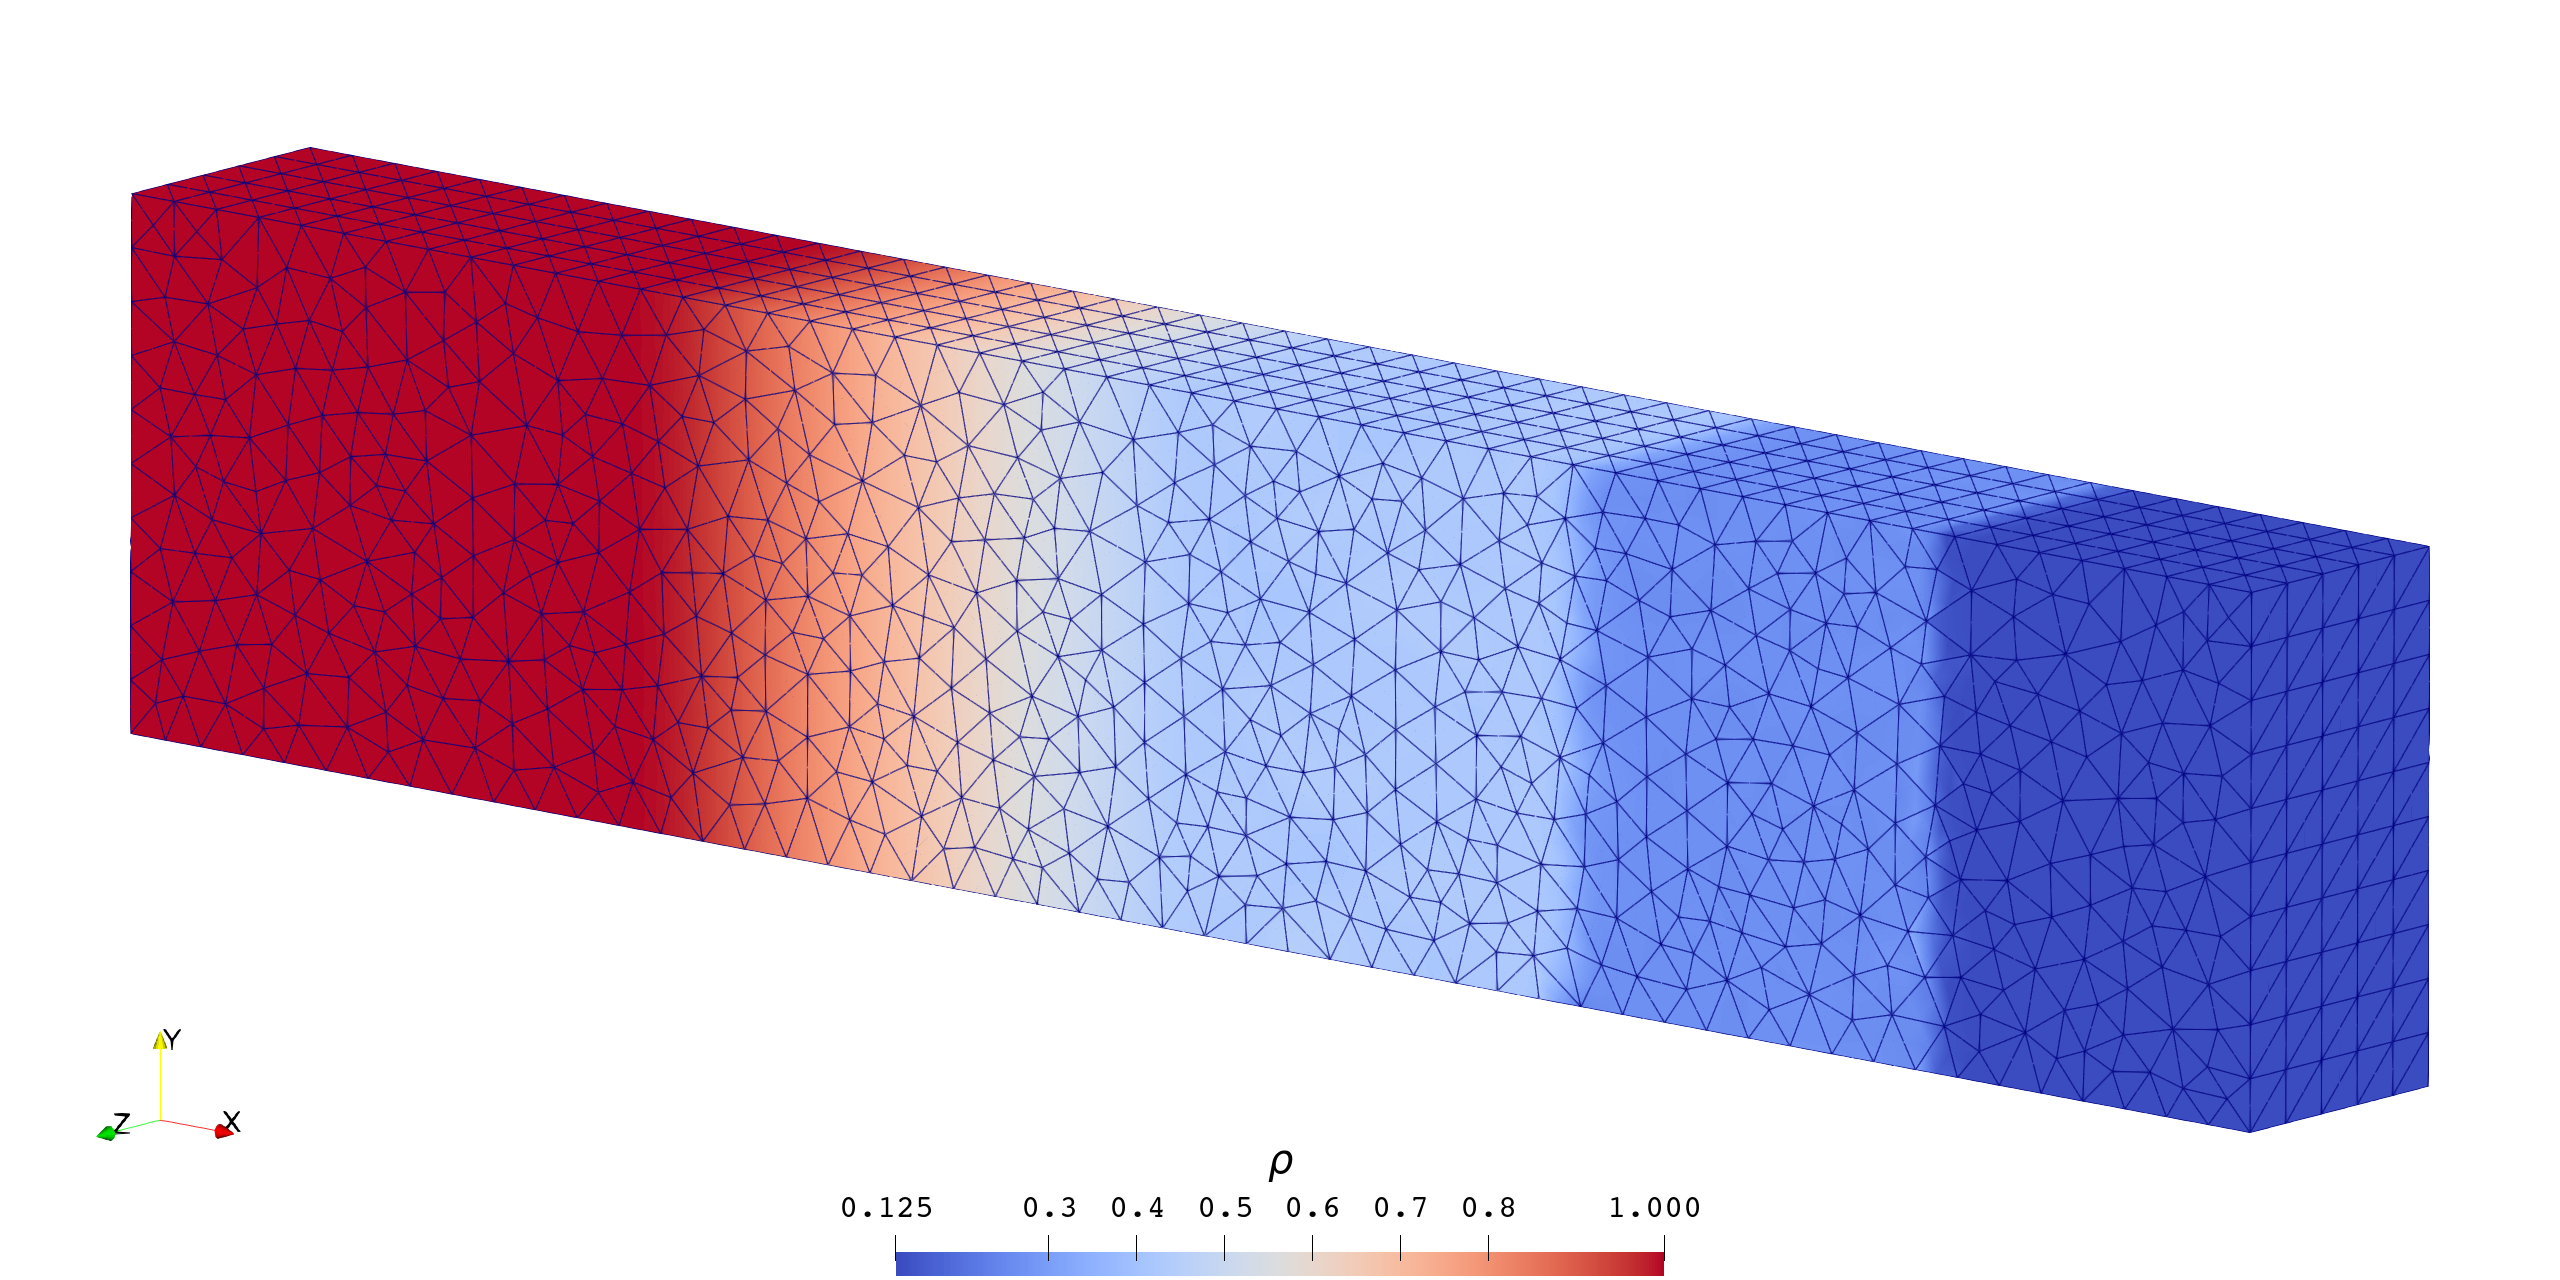
\includegraphics[width=1\textwidth]{figures/shock_tubes/sod/contour_tetra}

\caption{\label{fig:sod_contour}Third-order solution of $\rho(t=1.0)$ in
Problem \ref{prob:sod}.}
\end{figure}

\begin{figure}
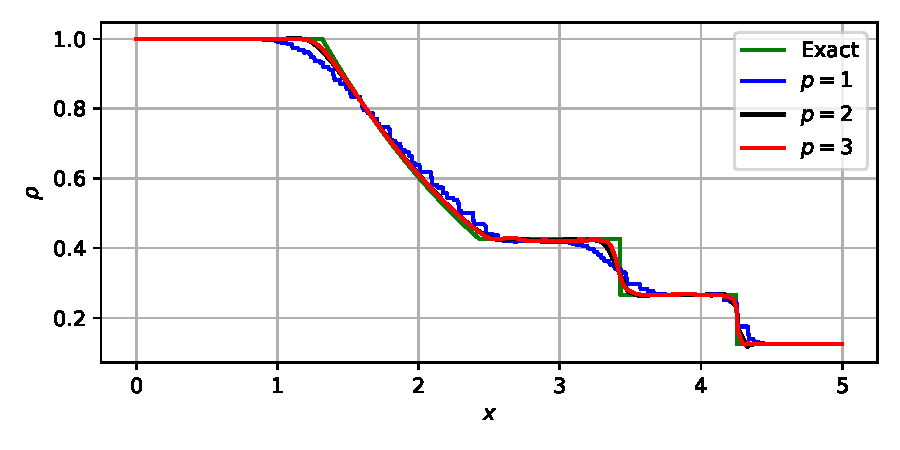
\includegraphics[width=1\textwidth]{figures/shock_tubes/sod/result_tetra}

\caption{\label{fig:sod_p}Comparison between solutions of $\rho(t=1.0)$ in
Problem \ref{prob:sod}.}
\end{figure}

This is a classical problem of inviscid compressible flows. It contains
all the three types of discontinuities: a shock wave and a contact
discontinuity running towards the right and an expansion wave running
towards the left. In Figure \ref{fig:sod_contour}, we plot the density
contour given by our third-order solver with an \texttt{EigenWeno}
limiter. In Figure \ref{fig:sod_p}, we compare the density distributions
given by various solvers along the longitudinal axis (on which $y=0.5$
and $z=0.25$) of the box. The accuracy of our solvers and the effect
of $p$-refinement are clear in these figures.

It is predictable that both mesh refinement (decreasing $h$) and
order increment (increasing $p$) can help to improve accuracy. To
compare the performance of solvers with different orders more fairly,
it is better to use finer meshes for running lower-order solvers.
After a few trials, we find that solutions given by the $h$-$p$
pairs listed in Table \ref{tab:sod_performance} roughly have the
same level of accuracy, as shown in Figure \ref{fig:sod_h}. It is
clear, at least for Problem \ref{prob:sod}, that high-order solvers
are better than low-order ones in the sense of getting the same level
of accuracy with less time and space costs. Similar conclusions were
drawn in our previous work \citep{Pei_2022}, in which the $p=3$
solution of a linear advection problem on an $h\approx1/4$ mesh defeated
the $p=1$ solution of the same problem on an $h\approx1/32$ mesh
in accuracy but saved quite a lot of time. These encouraging results
justify our efforts to implement higher-order solvers.

\begin{table}[H]
\caption{\label{tab:sod_performance}Comparison between time costs and file
sizes of various $h$-$p$ pairs.}

\begin{tabular*}{1\textwidth}{@{\extracolsep{\fill}}>{\centering}p{0.1\textwidth}>{\centering}p{0.05\textwidth}>{\centering}p{0.1\textwidth}>{\centering}p{0.1\textwidth}>{\centering}p{0.15\textwidth}>{\centering}p{0.1\textwidth}}
\toprule 
$h$ & $p$ & \#cells & \#steps & time cost & file size\tabularnewline
\midrule 
1/50 & 1 & 2469675 & 1500 & 1492.16 s & 1.23 GB\tabularnewline
1/18 & 2 & 117045 & 500 & 279.119 s & 213 MB\tabularnewline
1/10 & 3 & 19815 & 250 & 201.034 s & 89.1 MB\tabularnewline
\bottomrule
\end{tabular*}
\end{table}

\begin{figure}
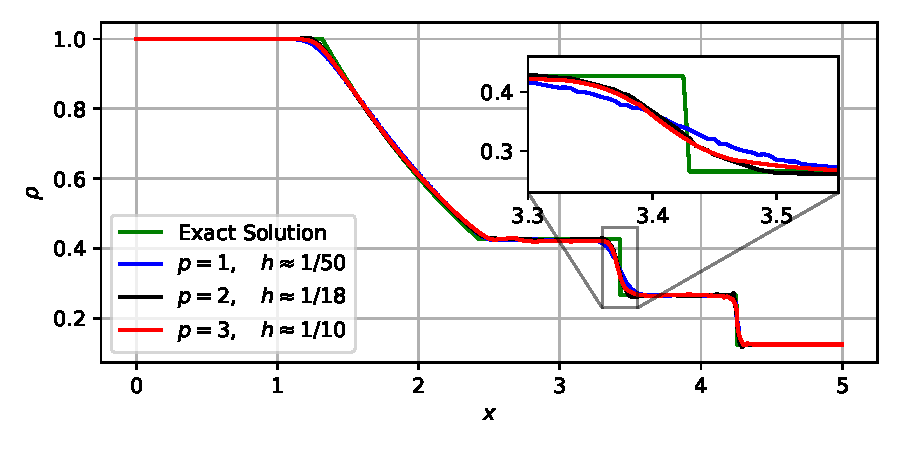
\includegraphics[width=1\textwidth]{figures/shock_tubes/sod/h_vary_tetra}

\caption{\label{fig:sod_h}Comparison between solutions given by various $h$-$p$
pairs.}
\end{figure}

\begin{Problem}
[Lax]\label{prob:lax}Solve the Euler system (Equation \ref{eq:euler_system})
for $t\in[0.0,0.6]$ with the initial condition

\[
\begin{bmatrix}\rho & u & v & w & p\end{bmatrix}_{t=0}=\begin{cases}
\begin{bmatrix}0.445 & 0.698 & 0.000 & 0.000 & 3.528\end{bmatrix} & x<2.5\\
\begin{bmatrix}0.500 & 0.000 & 0.000 & 0.000 & 0.571\end{bmatrix} & x>2.5
\end{cases}
\]
\end{Problem}

\begin{figure}
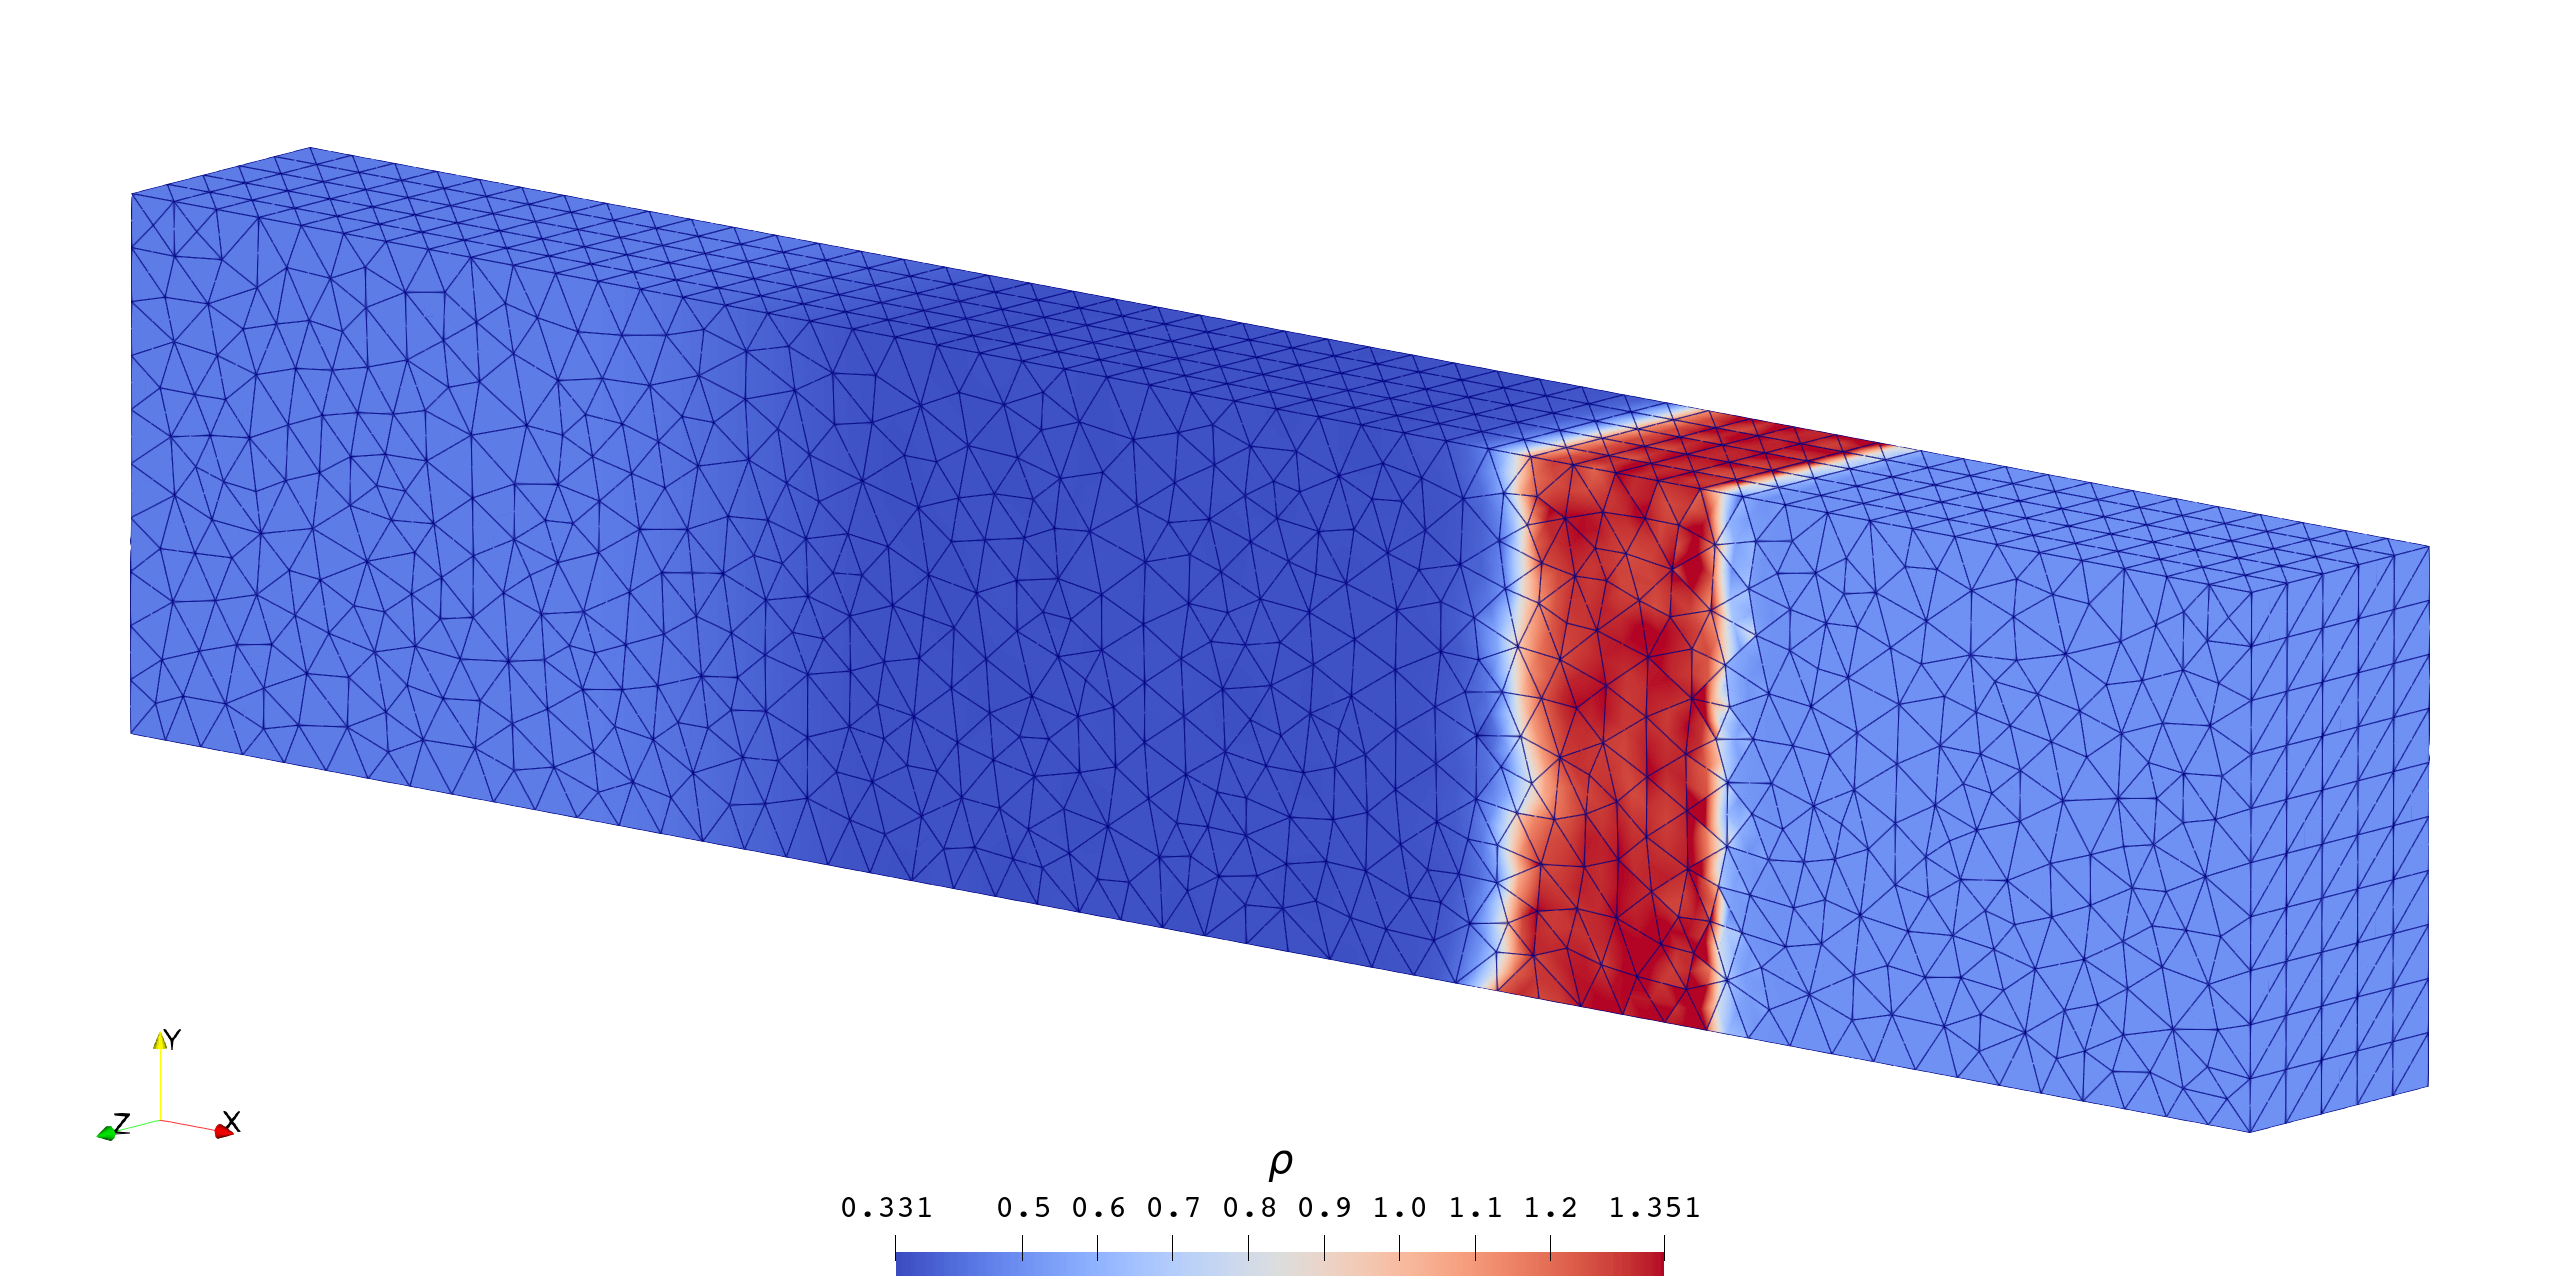
\includegraphics[width=1\textwidth]{figures/shock_tubes/lax/contour_tetra}

\caption{\label{fig:lax_contour}Third-order solution of $\rho(t=0.5)$ in
Problem \ref{prob:lax}.}
\end{figure}

\begin{figure}
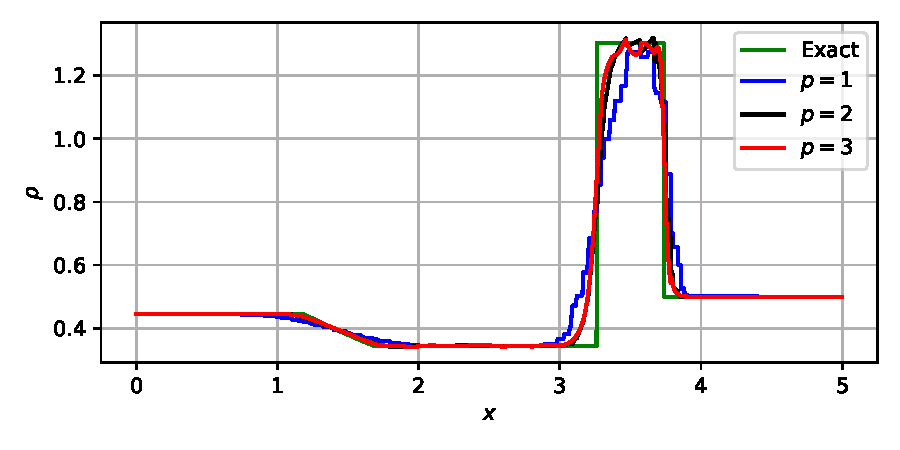
\includegraphics[width=1\textwidth]{figures/shock_tubes/lax/result_tetra}

\caption{\label{fig:lax}Comparison between solutions of $\rho(t=0.5)$ in
Problem \ref{prob:lax}.}
\end{figure}

This is another problem that involves all the three types of discontinuities.
It is more difficult than the previous one in the sense that its solution
contains values beyond the range of initial values and the discontinuities
are much steeper. As before, we plot the density contour of our third-order
solution in Figure \ref{fig:lax_contour} and compare the density
distributions given by various solvers in Figure \ref{fig:lax}. Both
figures demonstrate the effect of $p$-refinement and the ability
of our high-order solvers to suppress numerical oscillations.
\begin{Problem}
[Vacuum]\label{prob:vacuum}Solve the Euler system (Equation \ref{eq:euler_system})
for $t\in[0.0,0.4]$ with the initial condition

\[
\begin{bmatrix}\rho & u & v & w & p\end{bmatrix}_{t=0}=\begin{cases}
\begin{bmatrix}1 & -4 & 0 & 0 & 0.4\end{bmatrix} & x<2.5\\
\begin{bmatrix}1 & +4 & 0 & 0 & 0.4\end{bmatrix} & x>2.5
\end{cases}
\]
\end{Problem}

\begin{figure}
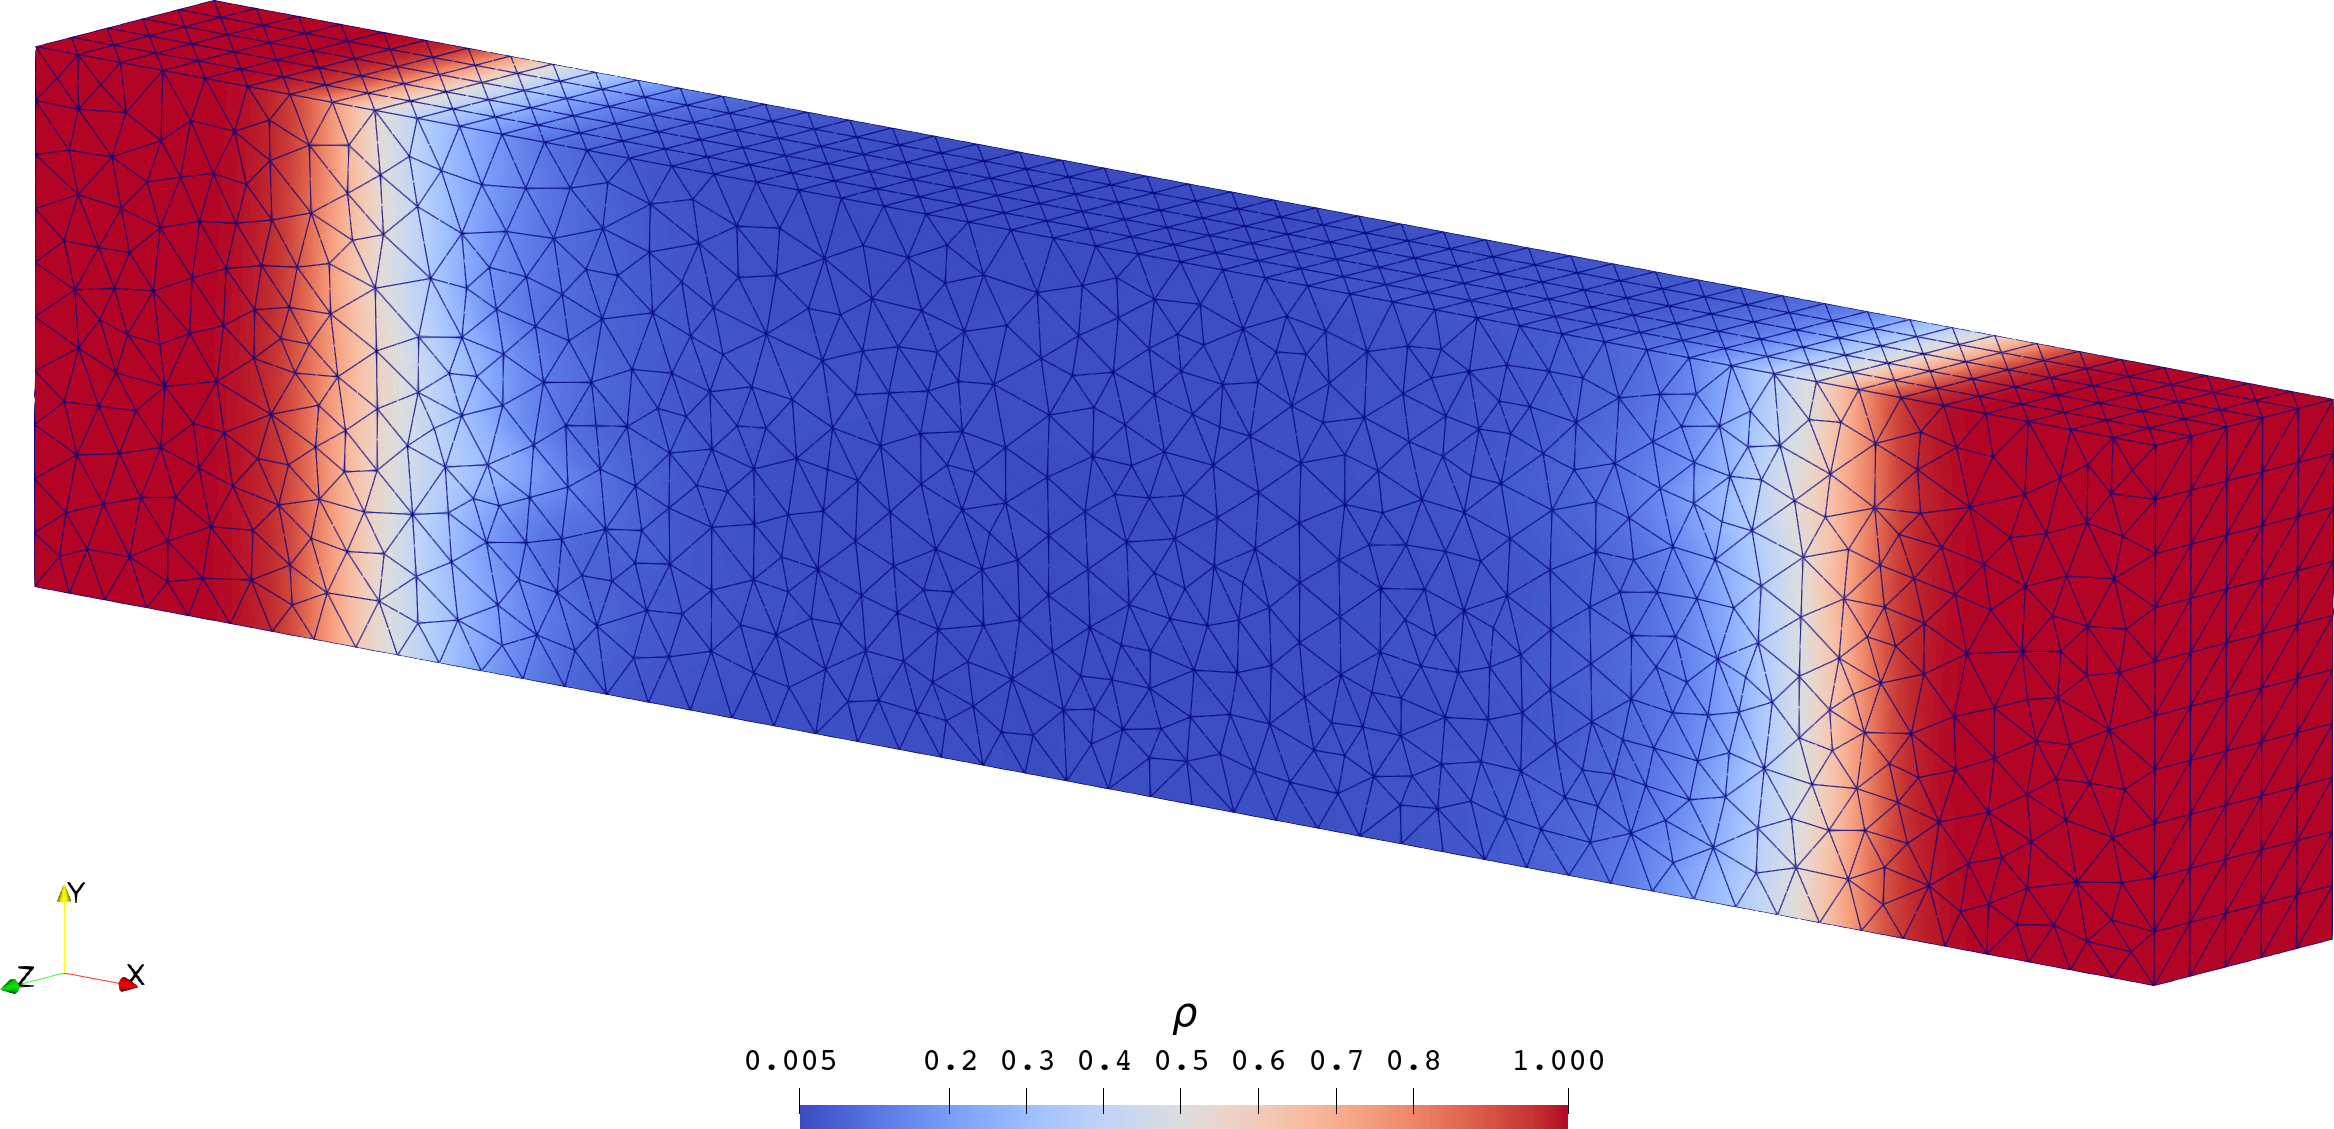
\includegraphics[width=1\textwidth]{figures/shock_tubes/vacuum/contour_tetra}

\caption{\label{fig:vacuum_contour}Third-order solution of $\rho(t=0.4)$
in Problem \ref{prob:vacuum}.}
\end{figure}

\begin{figure}
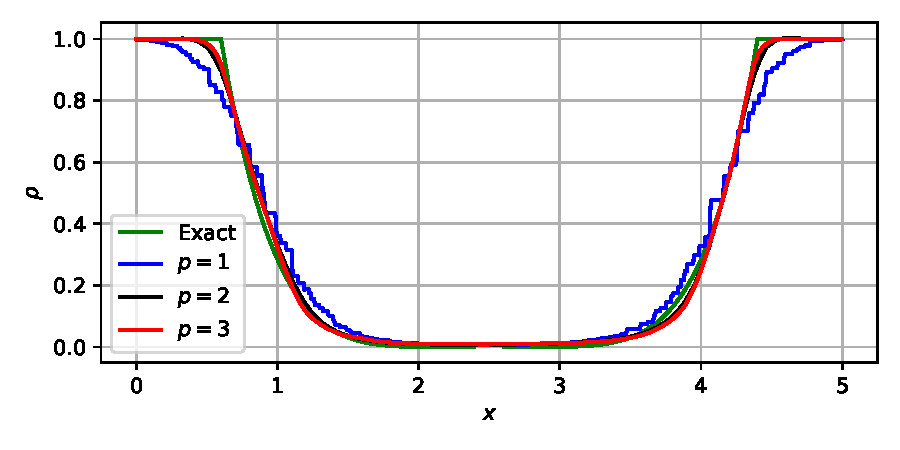
\includegraphics[width=1\textwidth]{figures/shock_tubes/vacuum/result_tetra}

\caption{\label{fig:vacuum}Comparison between solutions of $\rho(t=0.4)$
in Problem \ref{prob:vacuum}.}
\end{figure}

This problem is easier than the previous two in the sense that no
strong discontinuities (shock or contact discontinuity) occurs in
the solution. However, there is a region of vacuum, which does not
occur in the previous prolems, generated between the left- and right-running
expansion waves. The velocity $u$ inside the vacuumed region (denoted
by a $*$ in subscripts) is undefined, but its boundary values should
be determined from the left (denoted by an $L$ in subscripts) and
right (denoted by an $R$ in subscripts) initial values by the two
Riemann invariants:

\[
u_{*L}=u_{L}+\frac{2a_{L}}{\gamma-1},\qquad u_{*R}=u_{R}-\frac{2a_{R}}{\gamma-1}.
\]

See Section 4.6 in \citep{Toro_2009} for more detailed discussions.
Unfortunenately, approximate Riemann solvers usually (have to) neglect
this condition. For this reason, we use an exact Riemann solver to
obtain fluxes on cell boundaries. As before, we plot the results in
Figure \ref{fig:vacuum_contour} and Figure \ref{fig:vacuum}, which
again validate the correctness and robustness of our solvers.

\subsubsection{The Forward Step Problem}

This is a classical two-dimensional problem \citep{Woodward_1984},
but we treat it as a three-dimensional one:
\begin{Problem}
\label{prob:forward_step}Solve the Euler system (Equation \ref{eq:euler_system})
in a $[0,3]\times[0,1]\times[0,Z]$ box (representing a wind tunnel),
where the thickness $Z$ could be any positive value, with a $[0.6,3]\times[0,0.2]\times[0,Z]$
box removed (representing a forward-facing step). The $x=0$ surface
is open as an inlet and the $x=3$ surface is open as an outlet. All
other boundary surfaces are closed as solid walls. The initial condition
is given as a uniform state:

\[
\begin{bmatrix}\rho & u & v & w & p\end{bmatrix}_{t=0}=\begin{bmatrix}1.4 & 3.0 & 0.0 & 0.0 & 1.0\end{bmatrix}.
\]
\end{Problem}

\begin{figure}
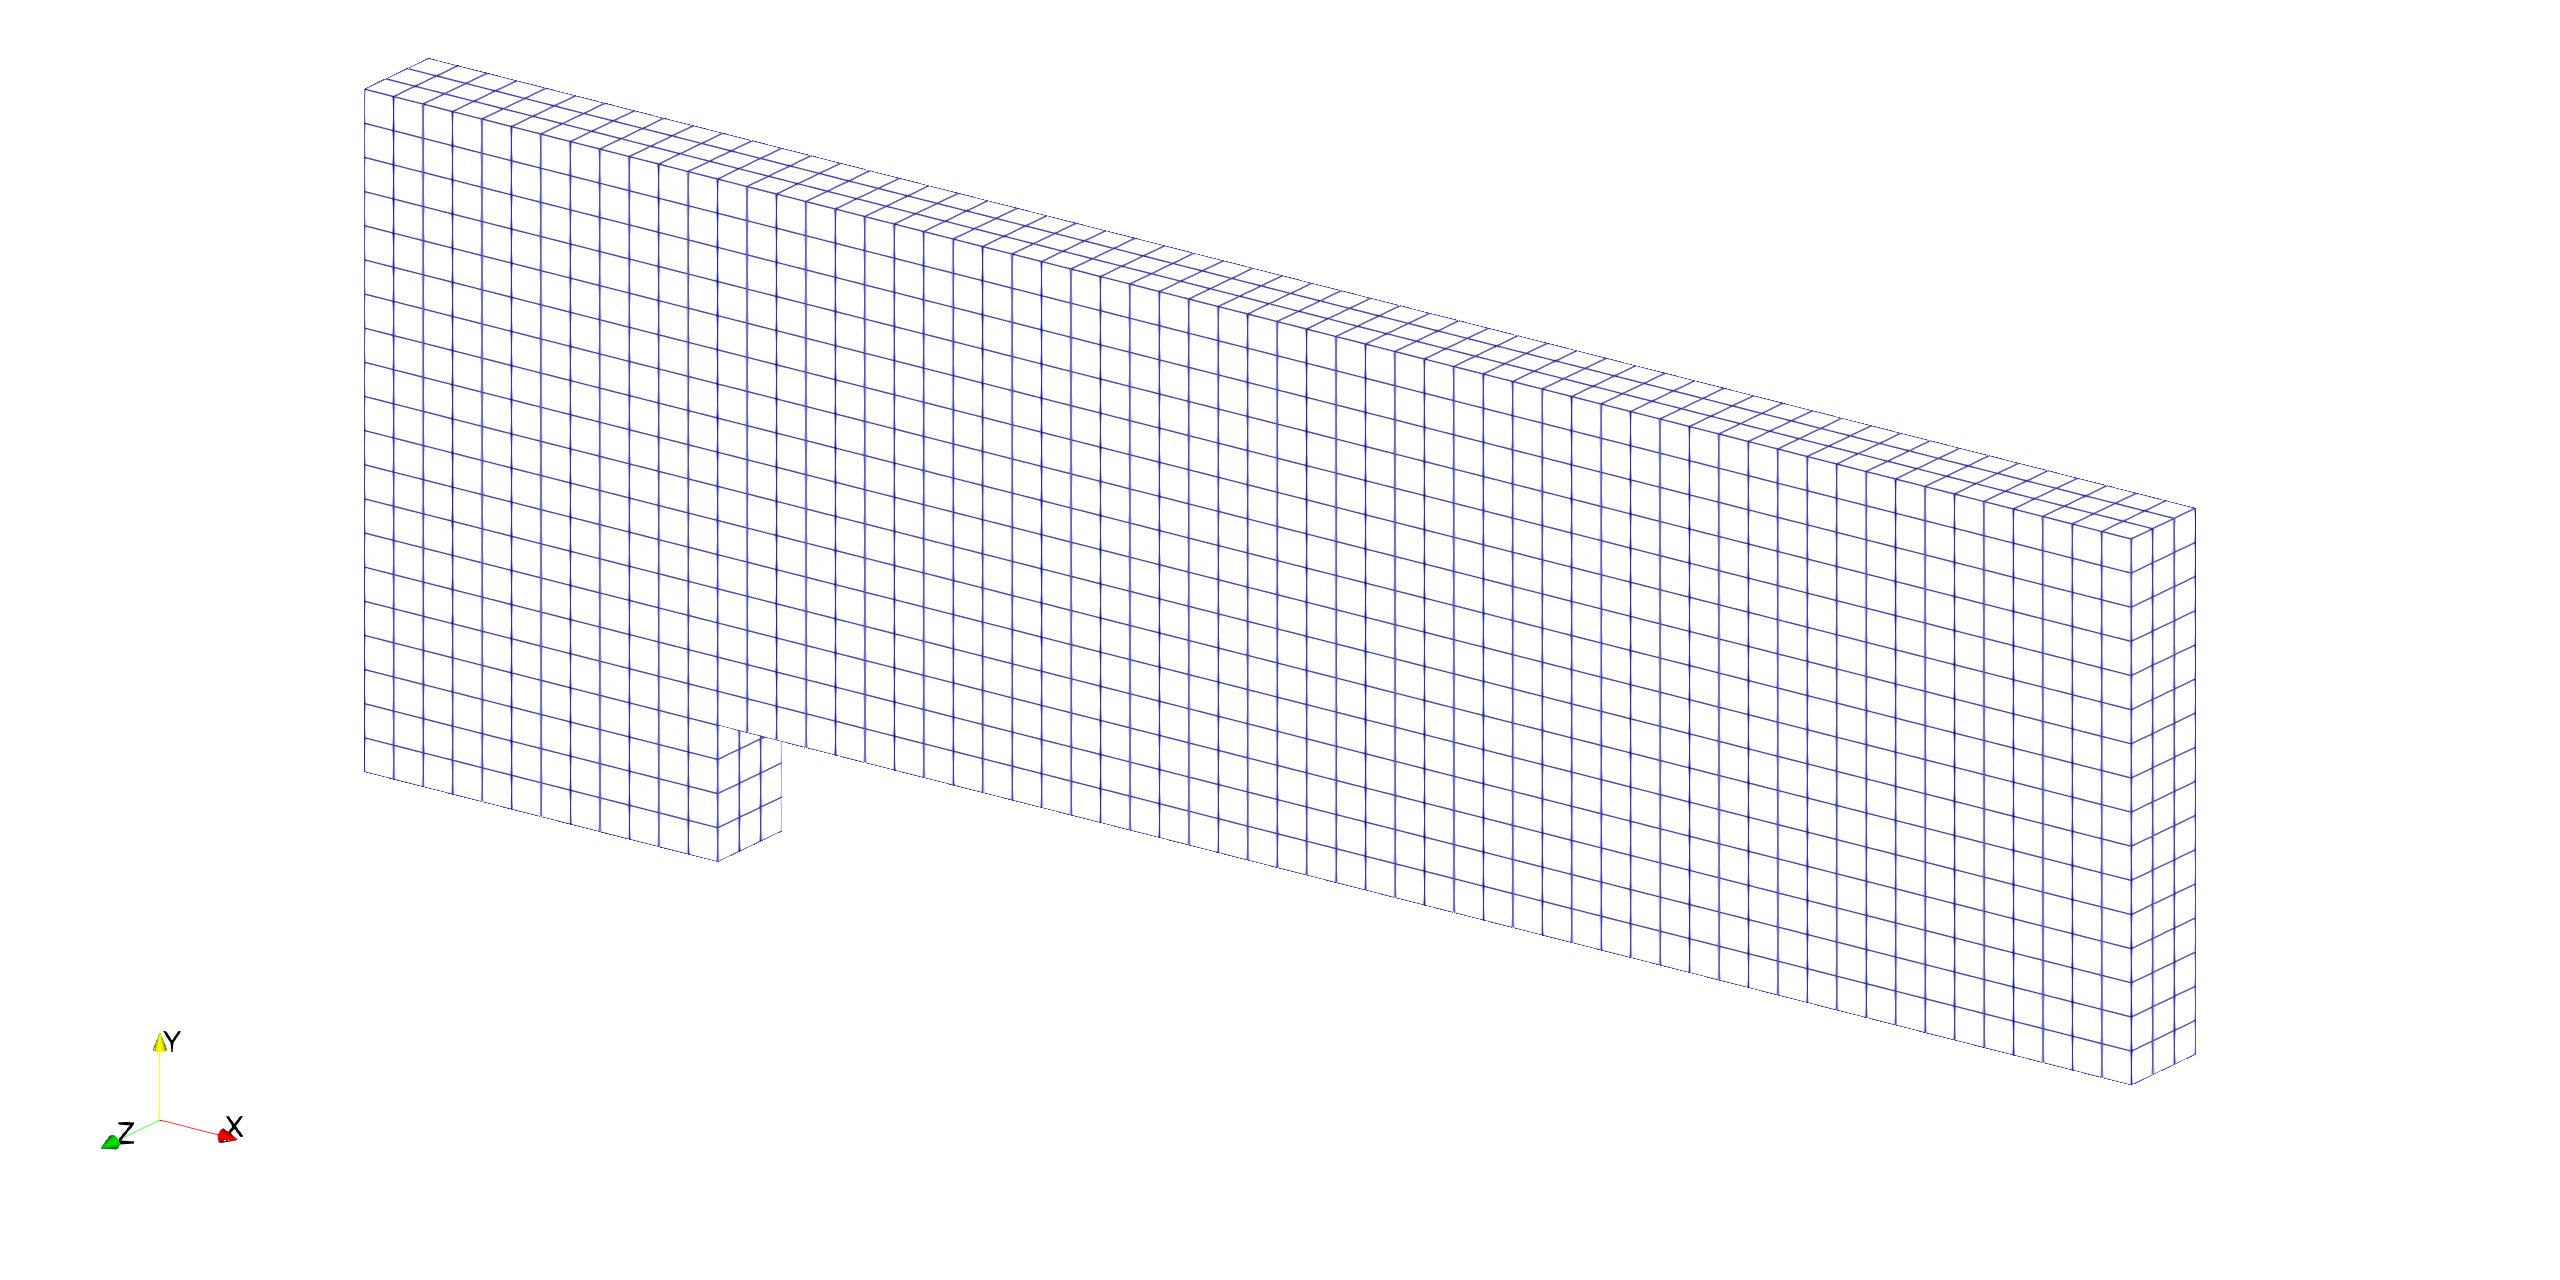
\includegraphics[width=1\textwidth]{figures/forward_step/mesh}

\caption{\label{fig:forward_step_domain}A coarse ($h=1/20$) mesh for solving
Problem \ref{prob:forward_step}. This mesh is too coarse to capture
details of the flow field but clear enough to demonstrate the distribution
of nodes and cells. Actually, we use a much finer ($h=1/200$) mesh
to produce Figures \ref{fig:forward_step_p=00003D3_t=00003D02e-1}--\ref{fig:forward_step_p=00003D3_t=00003D40e-1}.}
\end{figure}

To show the applicability of our solvers on structured meshes, we
solve this problem on meshes like the one in Figure \ref{fig:forward_step_domain}.
As a common practice, we plot the density contours at various time
steps in Figures \ref{fig:forward_step_p=00003D3_t=00003D02e-1}--\ref{fig:forward_step_p=00003D3_t=00003D40e-1}.

\begin{figure}
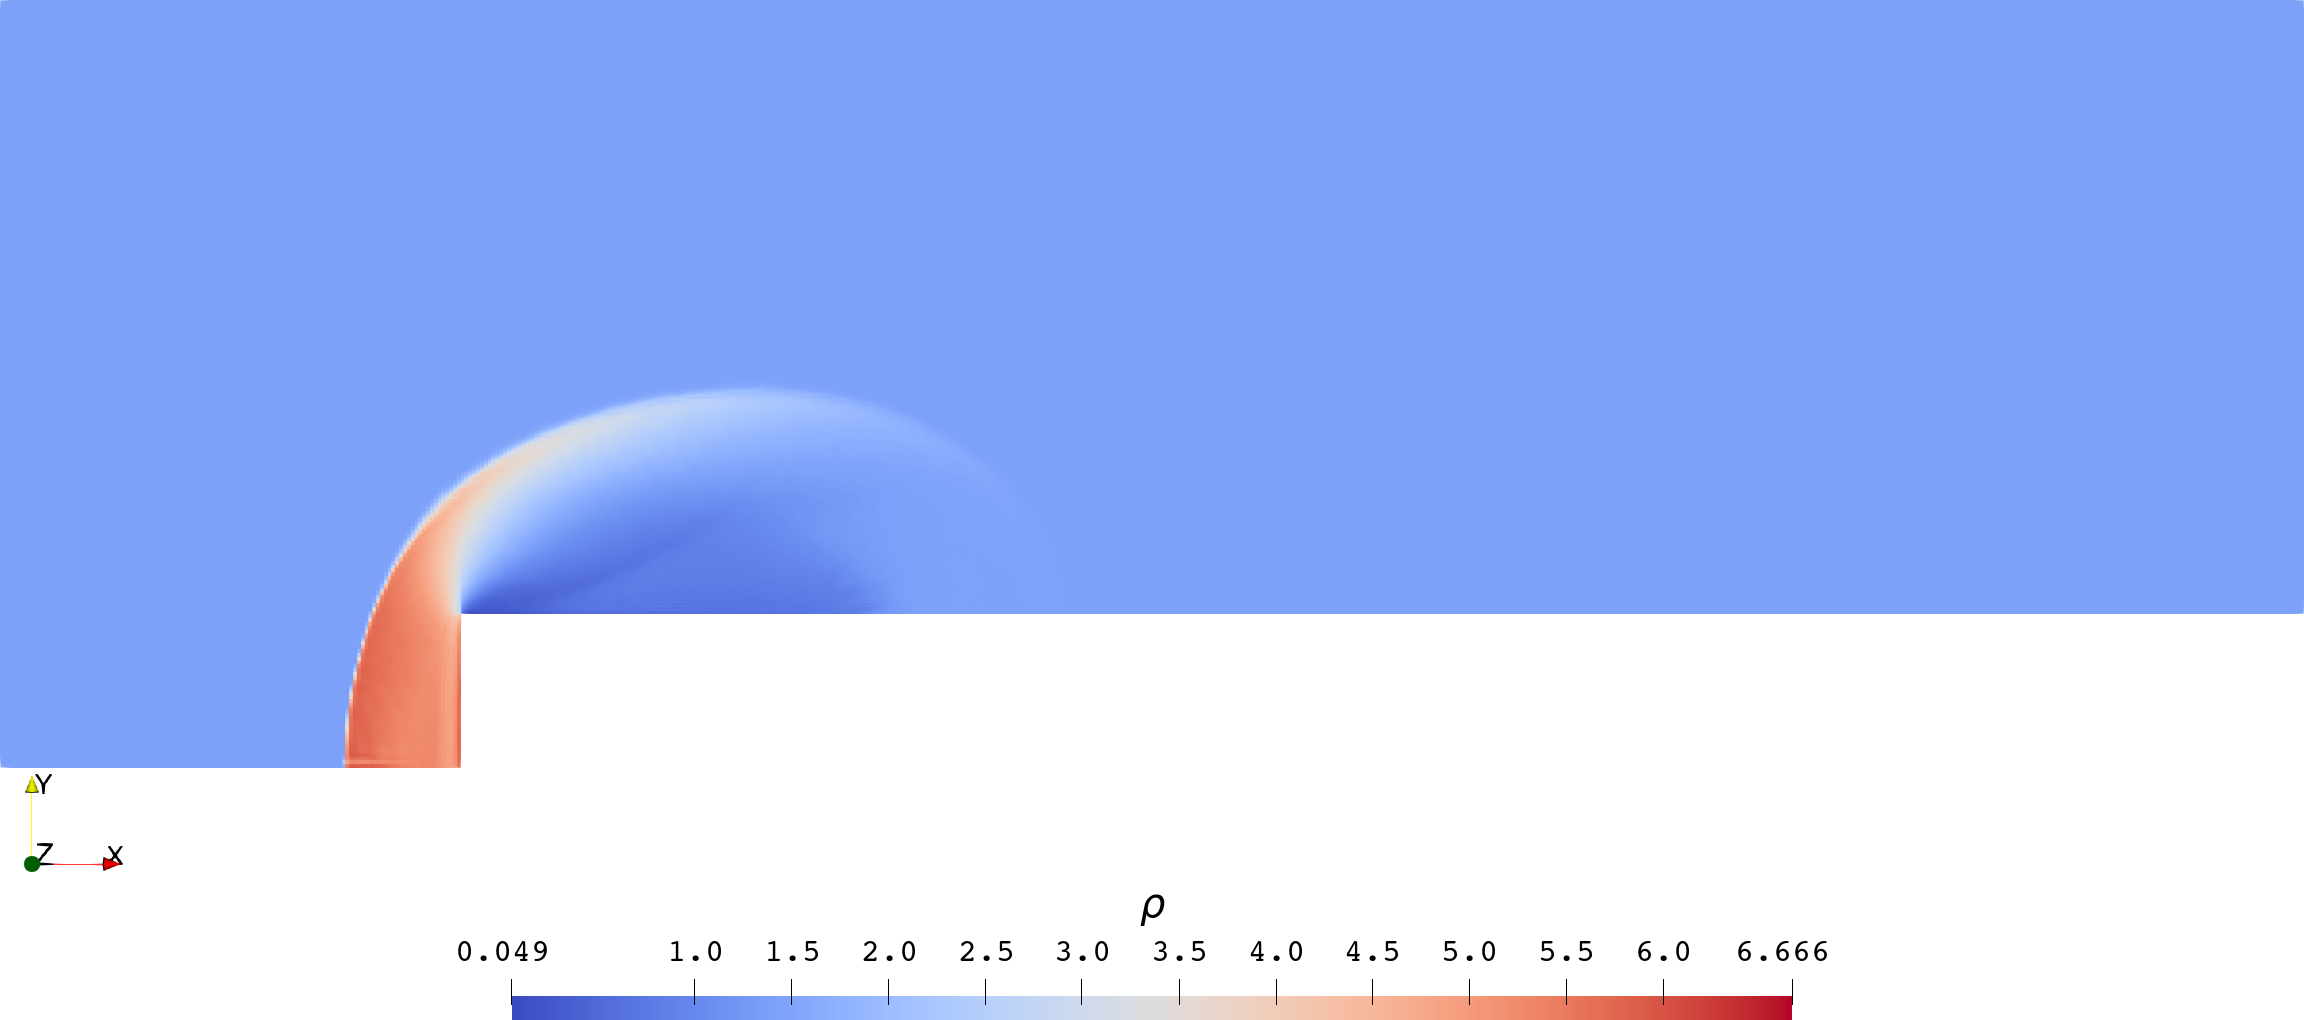
\includegraphics[width=1\textwidth]{figures/forward_step/p=3_t=02e-1}

\caption{\label{fig:forward_step_p=00003D3_t=00003D02e-1}Third-order solution
of Problem \ref{prob:forward_step} at $t=0.2$ on an $h=1/200$ mesh.}
\end{figure}

\begin{figure}
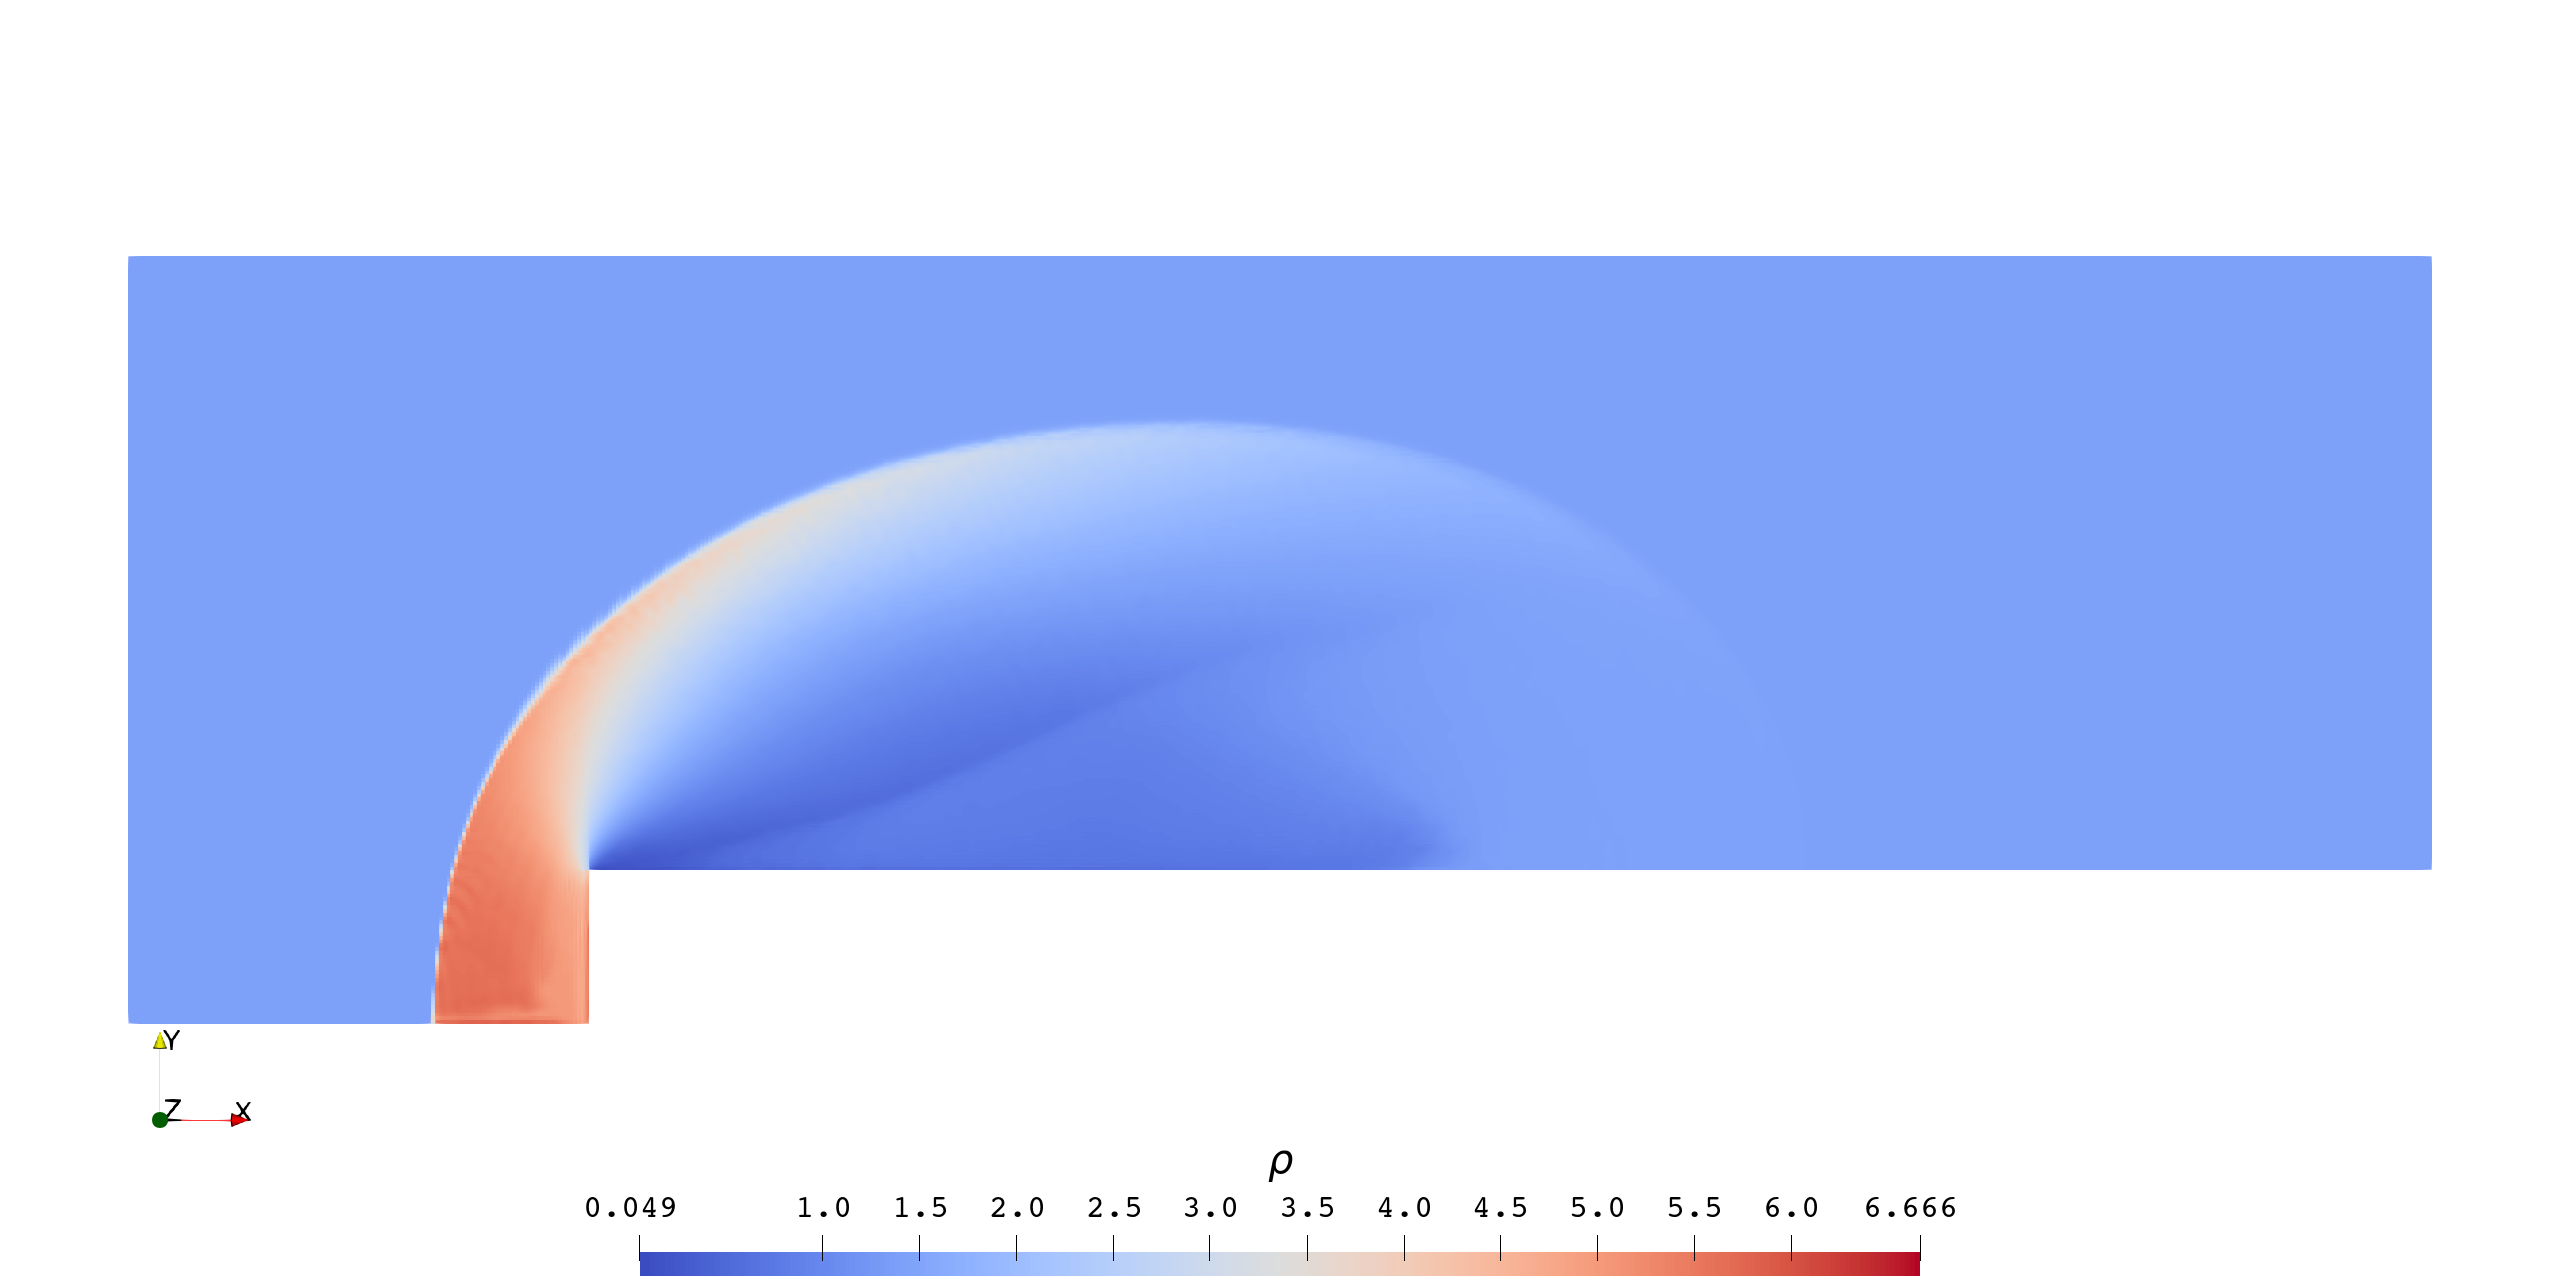
\includegraphics[width=1\textwidth]{figures/forward_step/p=3_t=04e-1}

\caption{\label{fig:forward_step_p=00003D3_t=00003D04e-1}Third-order solution
of Problem \ref{prob:forward_step} at $t=0.4$ on an $h=1/200$ mesh.}
\end{figure}

\begin{figure}
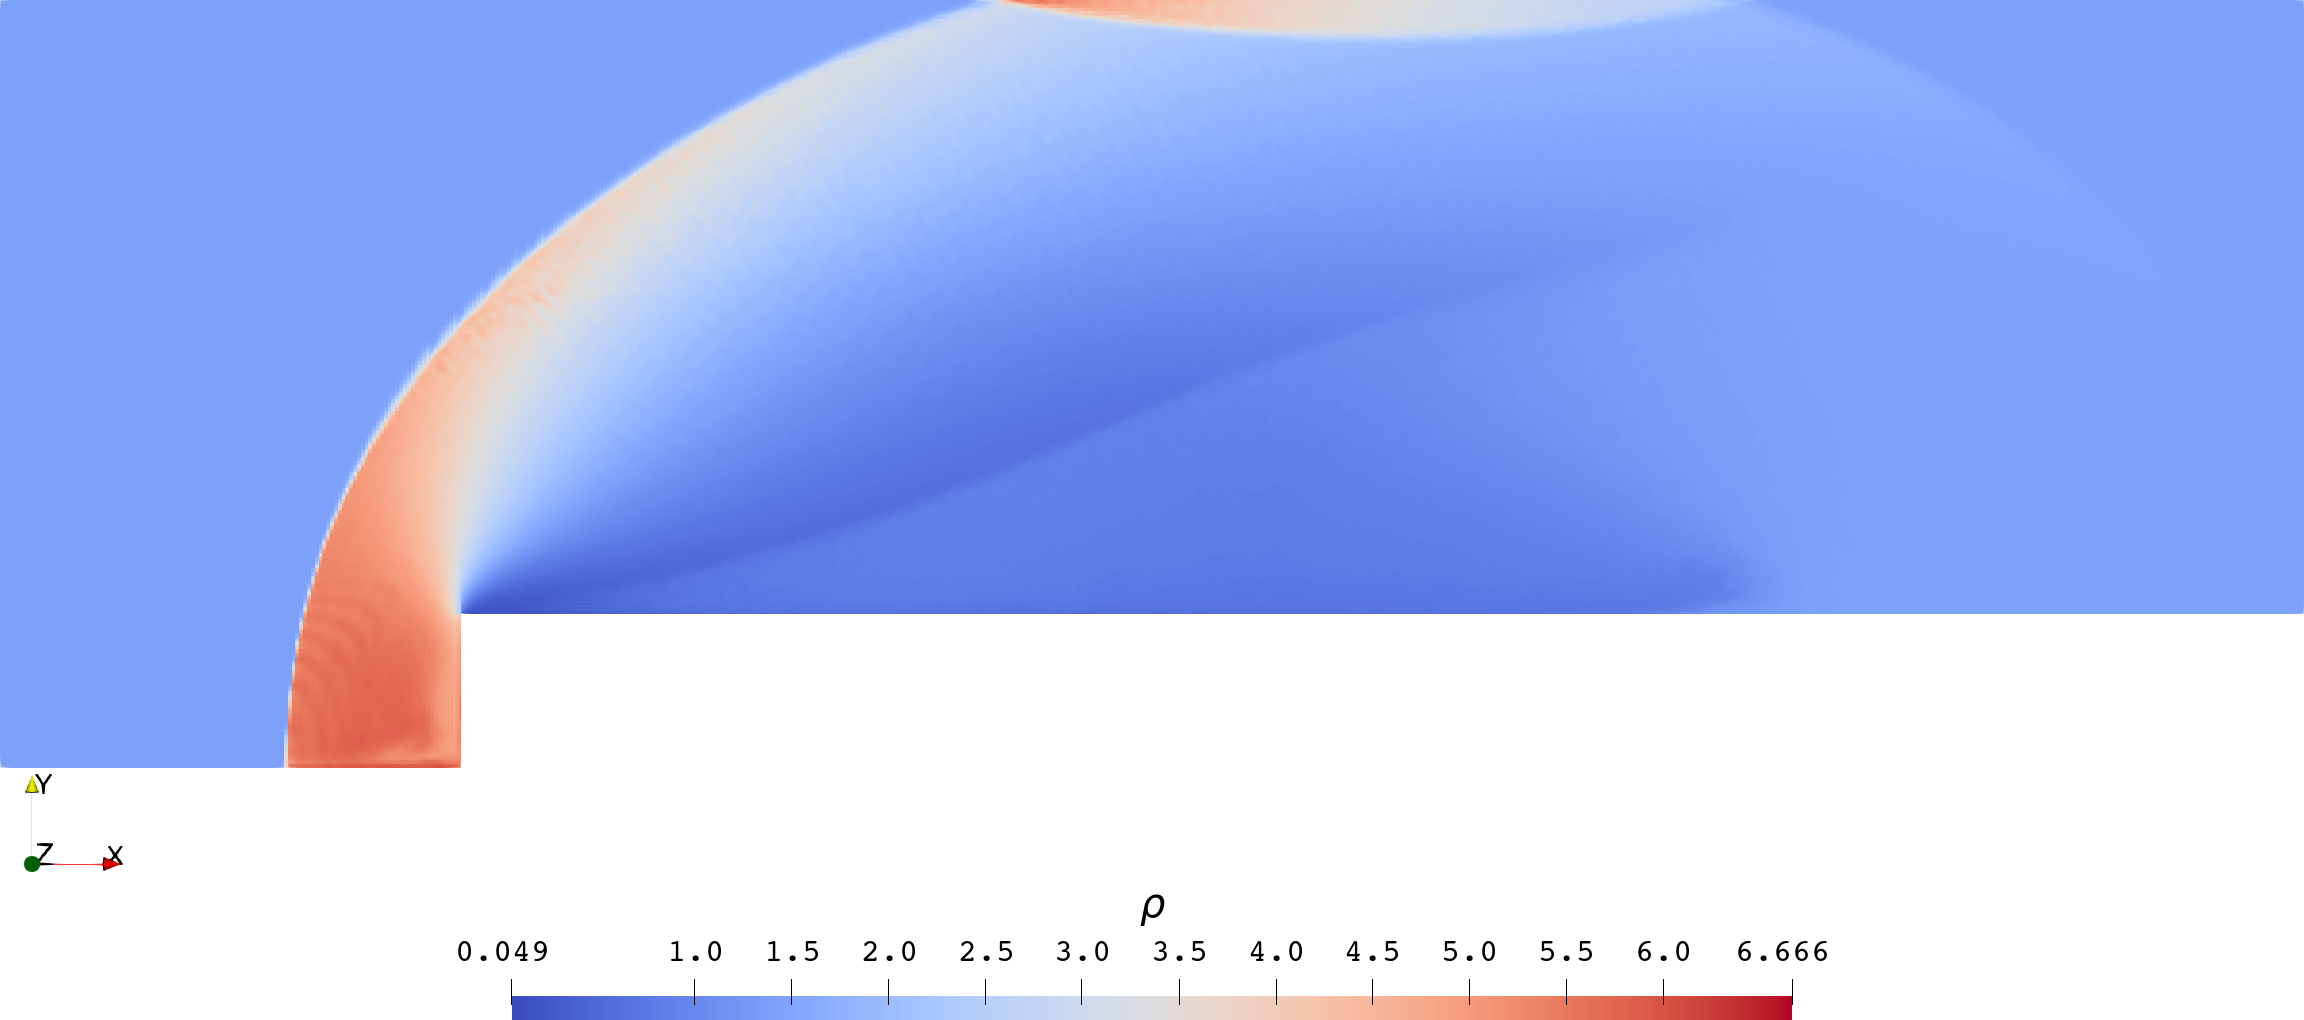
\includegraphics[width=1\textwidth]{figures/forward_step/p=3_t=06e-1}

\caption{\label{fig:forward_step_p=00003D3_t=00003D06e-1}Third-order solution
of Problem \ref{prob:forward_step} at $t=0.6$ on an $h=1/200$ mesh.}
\end{figure}

\begin{figure}
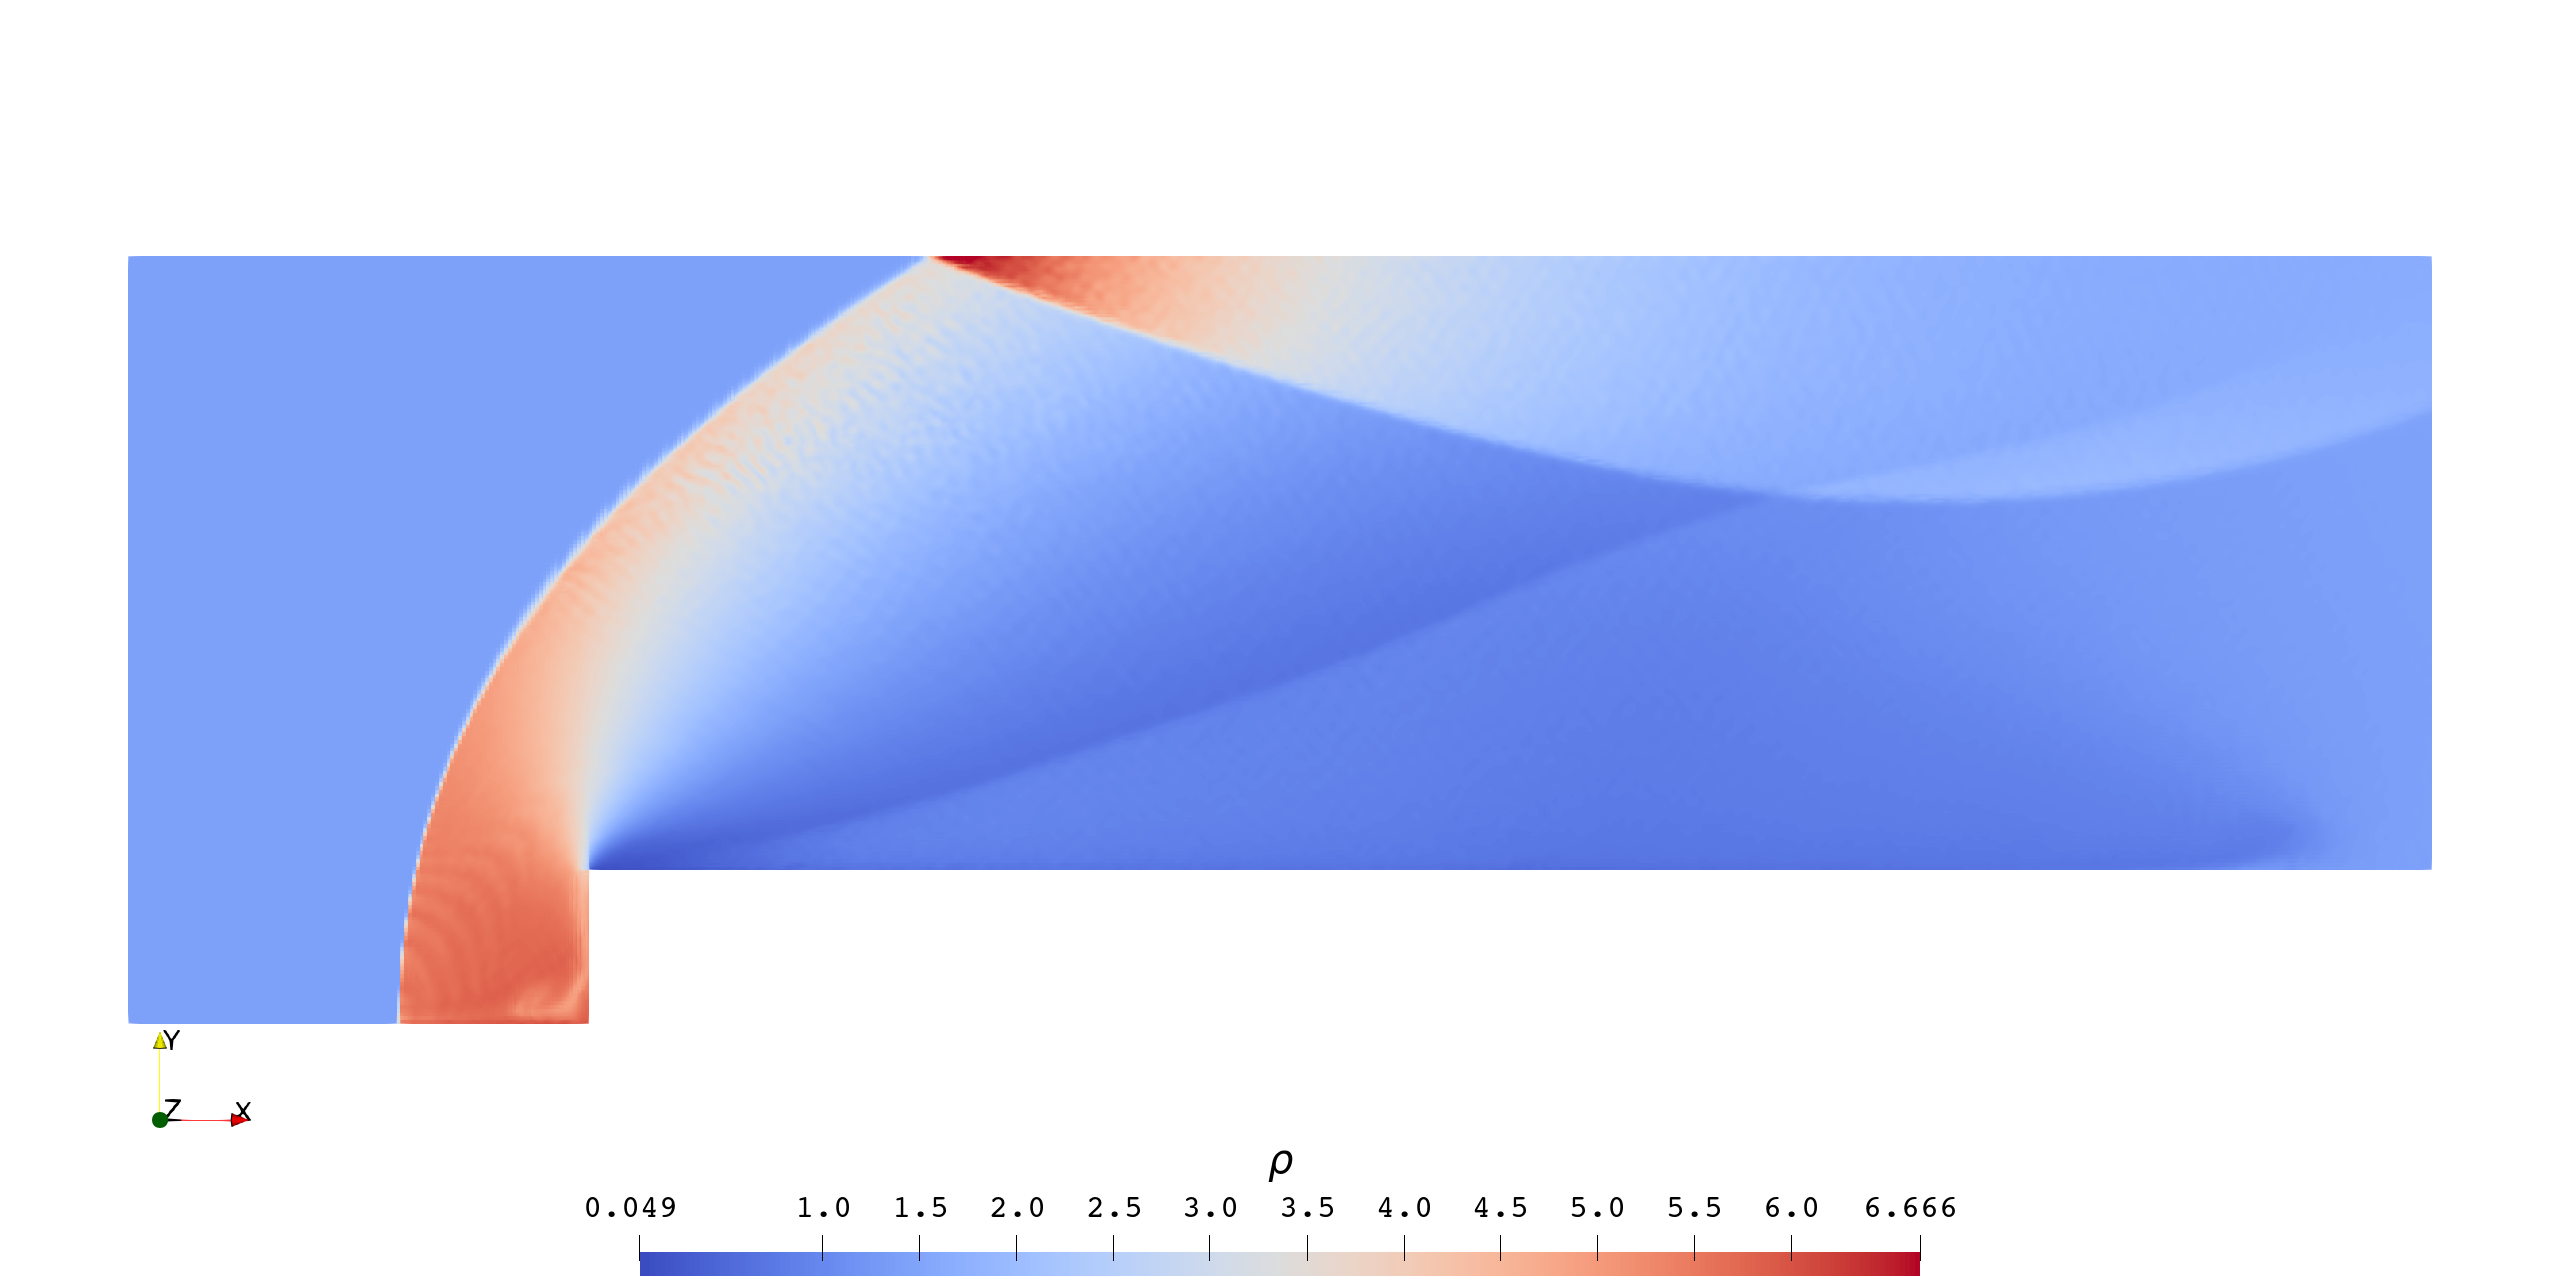
\includegraphics[width=1\textwidth]{figures/forward_step/p=3_t=08e-1}

\caption{\label{fig:forward_step_p=00003D3_t=00003D08e-1}Third-order solution
of Problem \ref{prob:forward_step} at $t=0.8$ on an $h=1/200$ mesh.}
\end{figure}

\begin{figure}
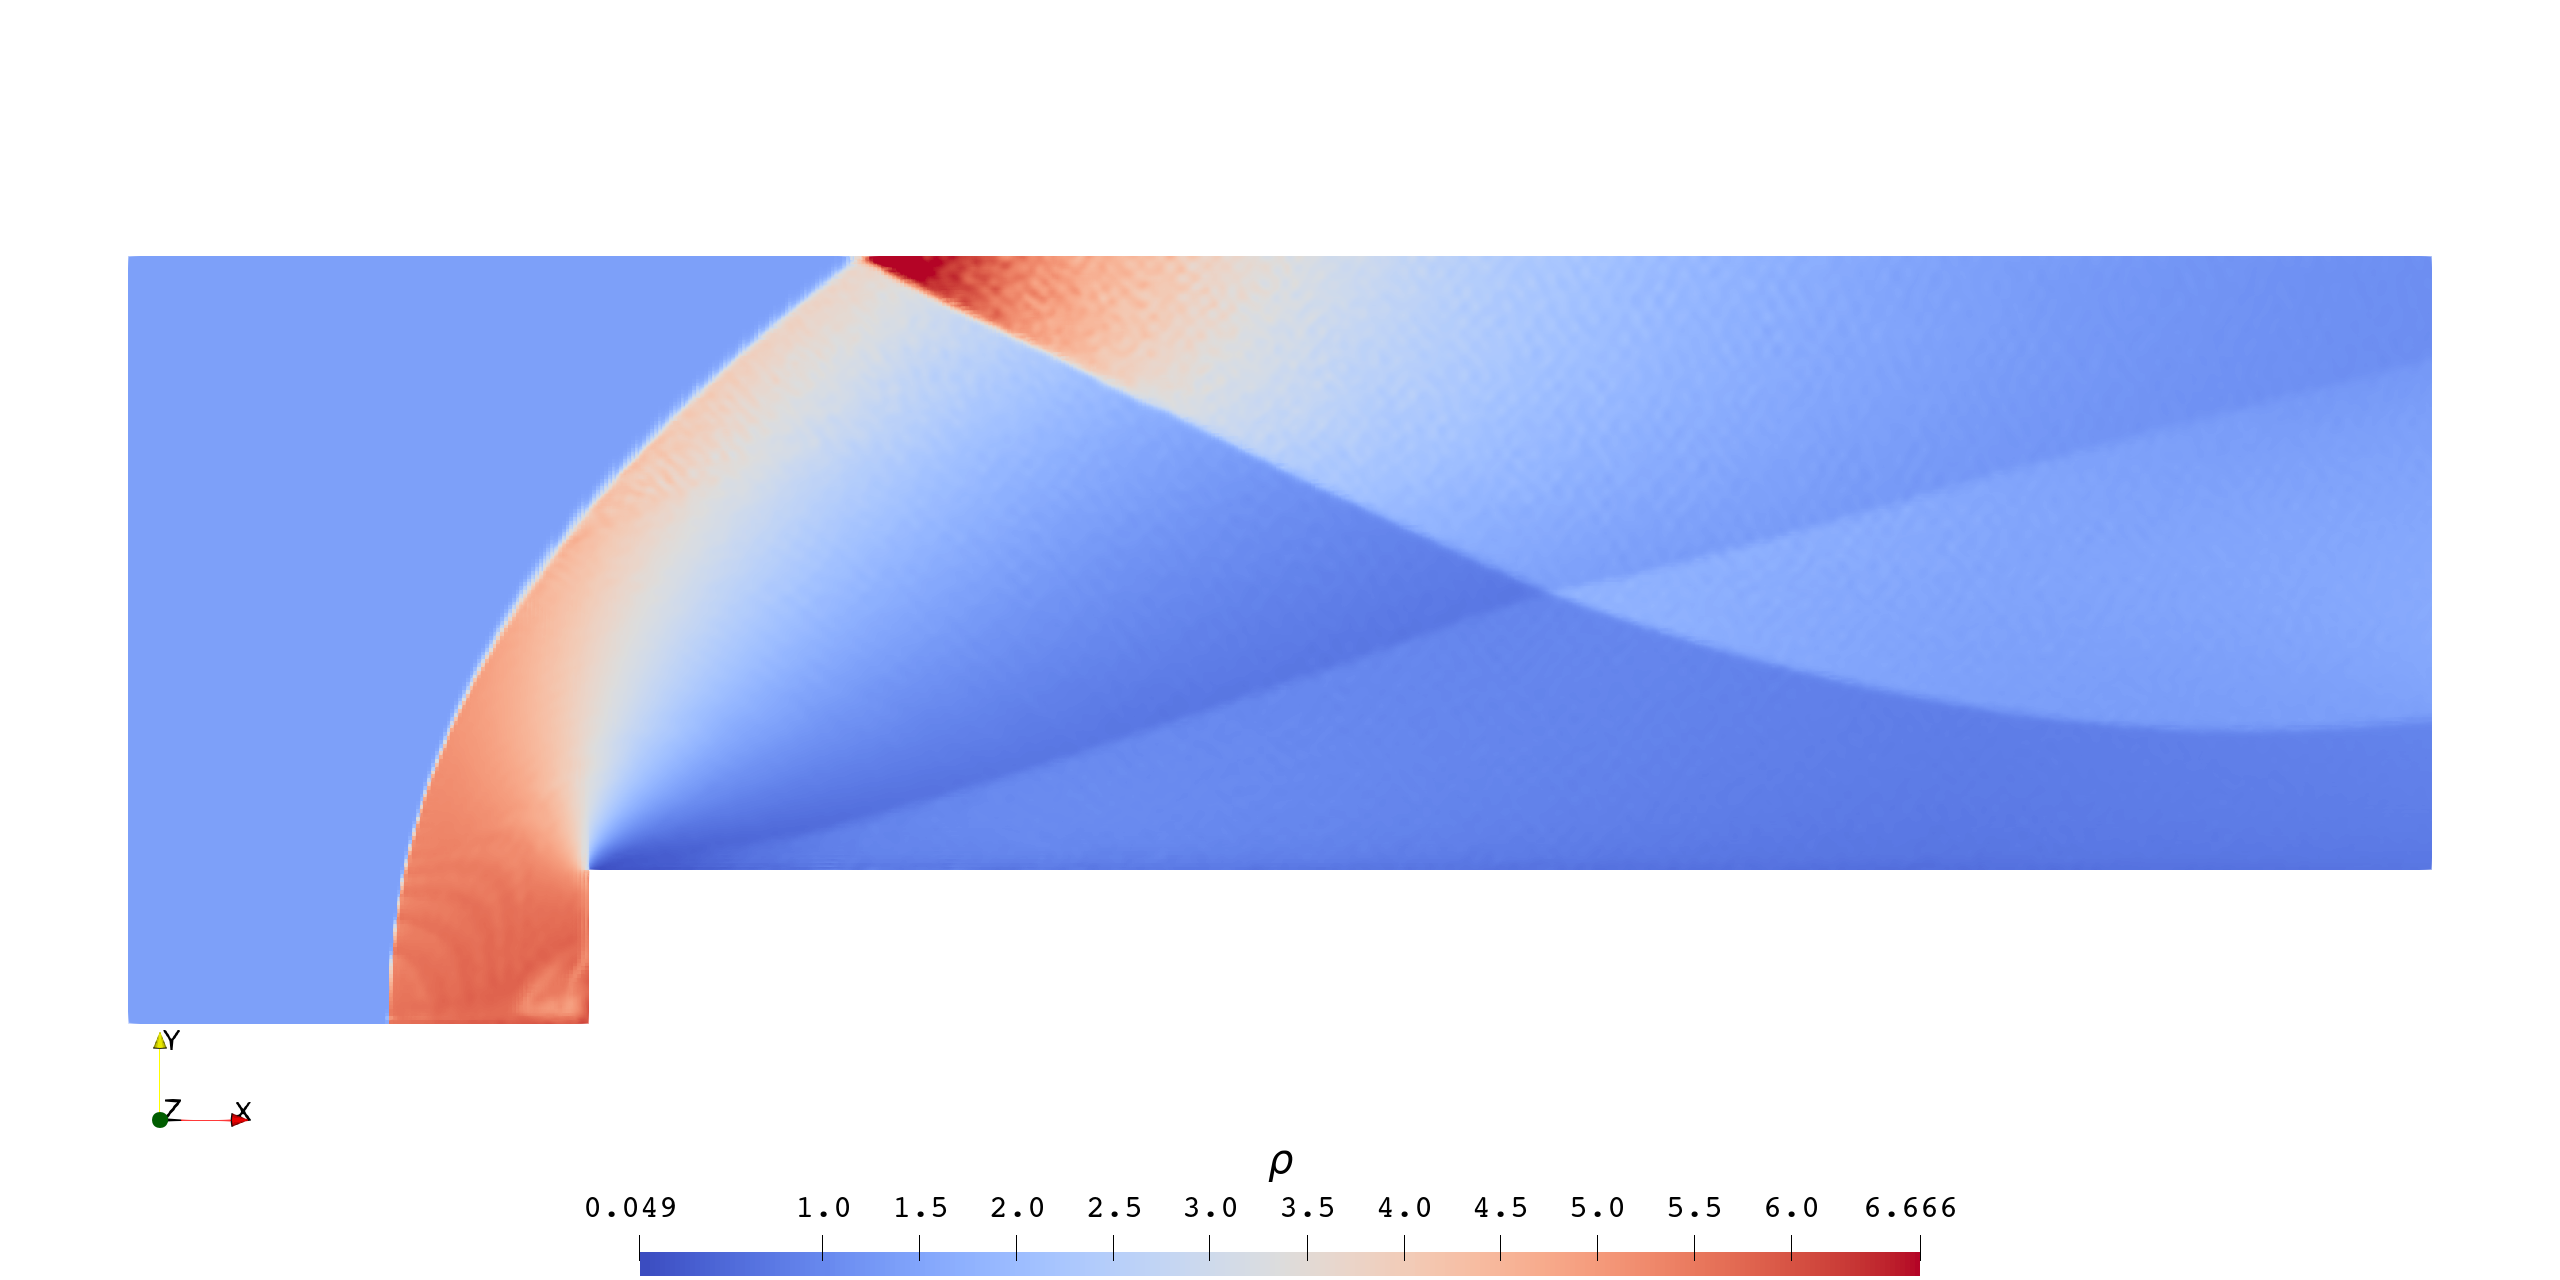
\includegraphics[width=1\textwidth]{figures/forward_step/p=3_t=10e-1}

\caption{\label{fig:forward_step_p=00003D3_t=00003D10e-1}Third-order solution
of Problem \ref{prob:forward_step} at $t=1.0$ on an $h=1/200$ mesh.}
\end{figure}

\begin{figure}
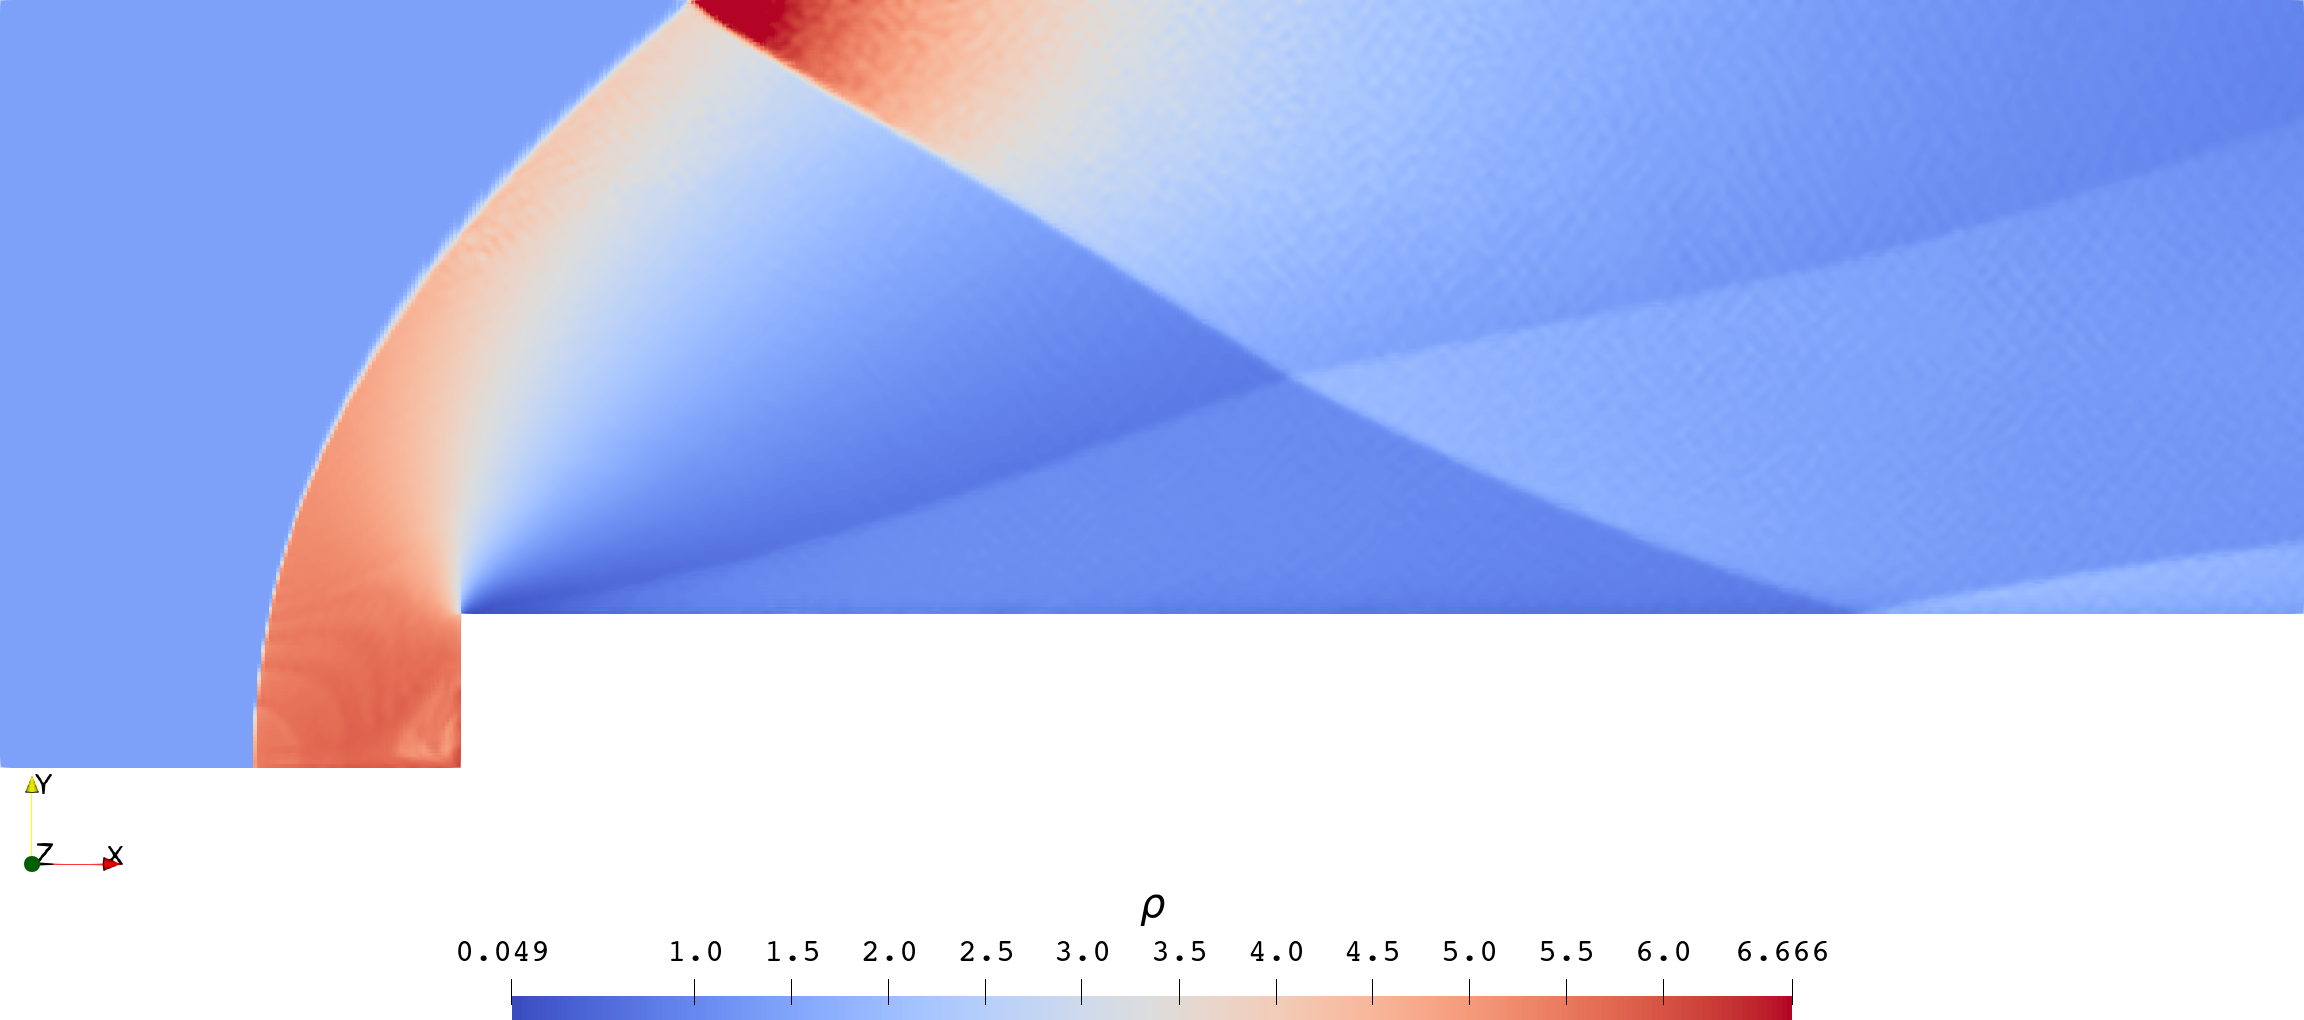
\includegraphics[width=1\textwidth]{figures/forward_step/p=3_t=12e-1}

\caption{\label{fig:forward_step_p=00003D3_t=00003D12e-1}Third-order solution
of Problem \ref{prob:forward_step} at $t=1.2$ on an $h=1/200$ mesh.}
\end{figure}

\begin{figure}
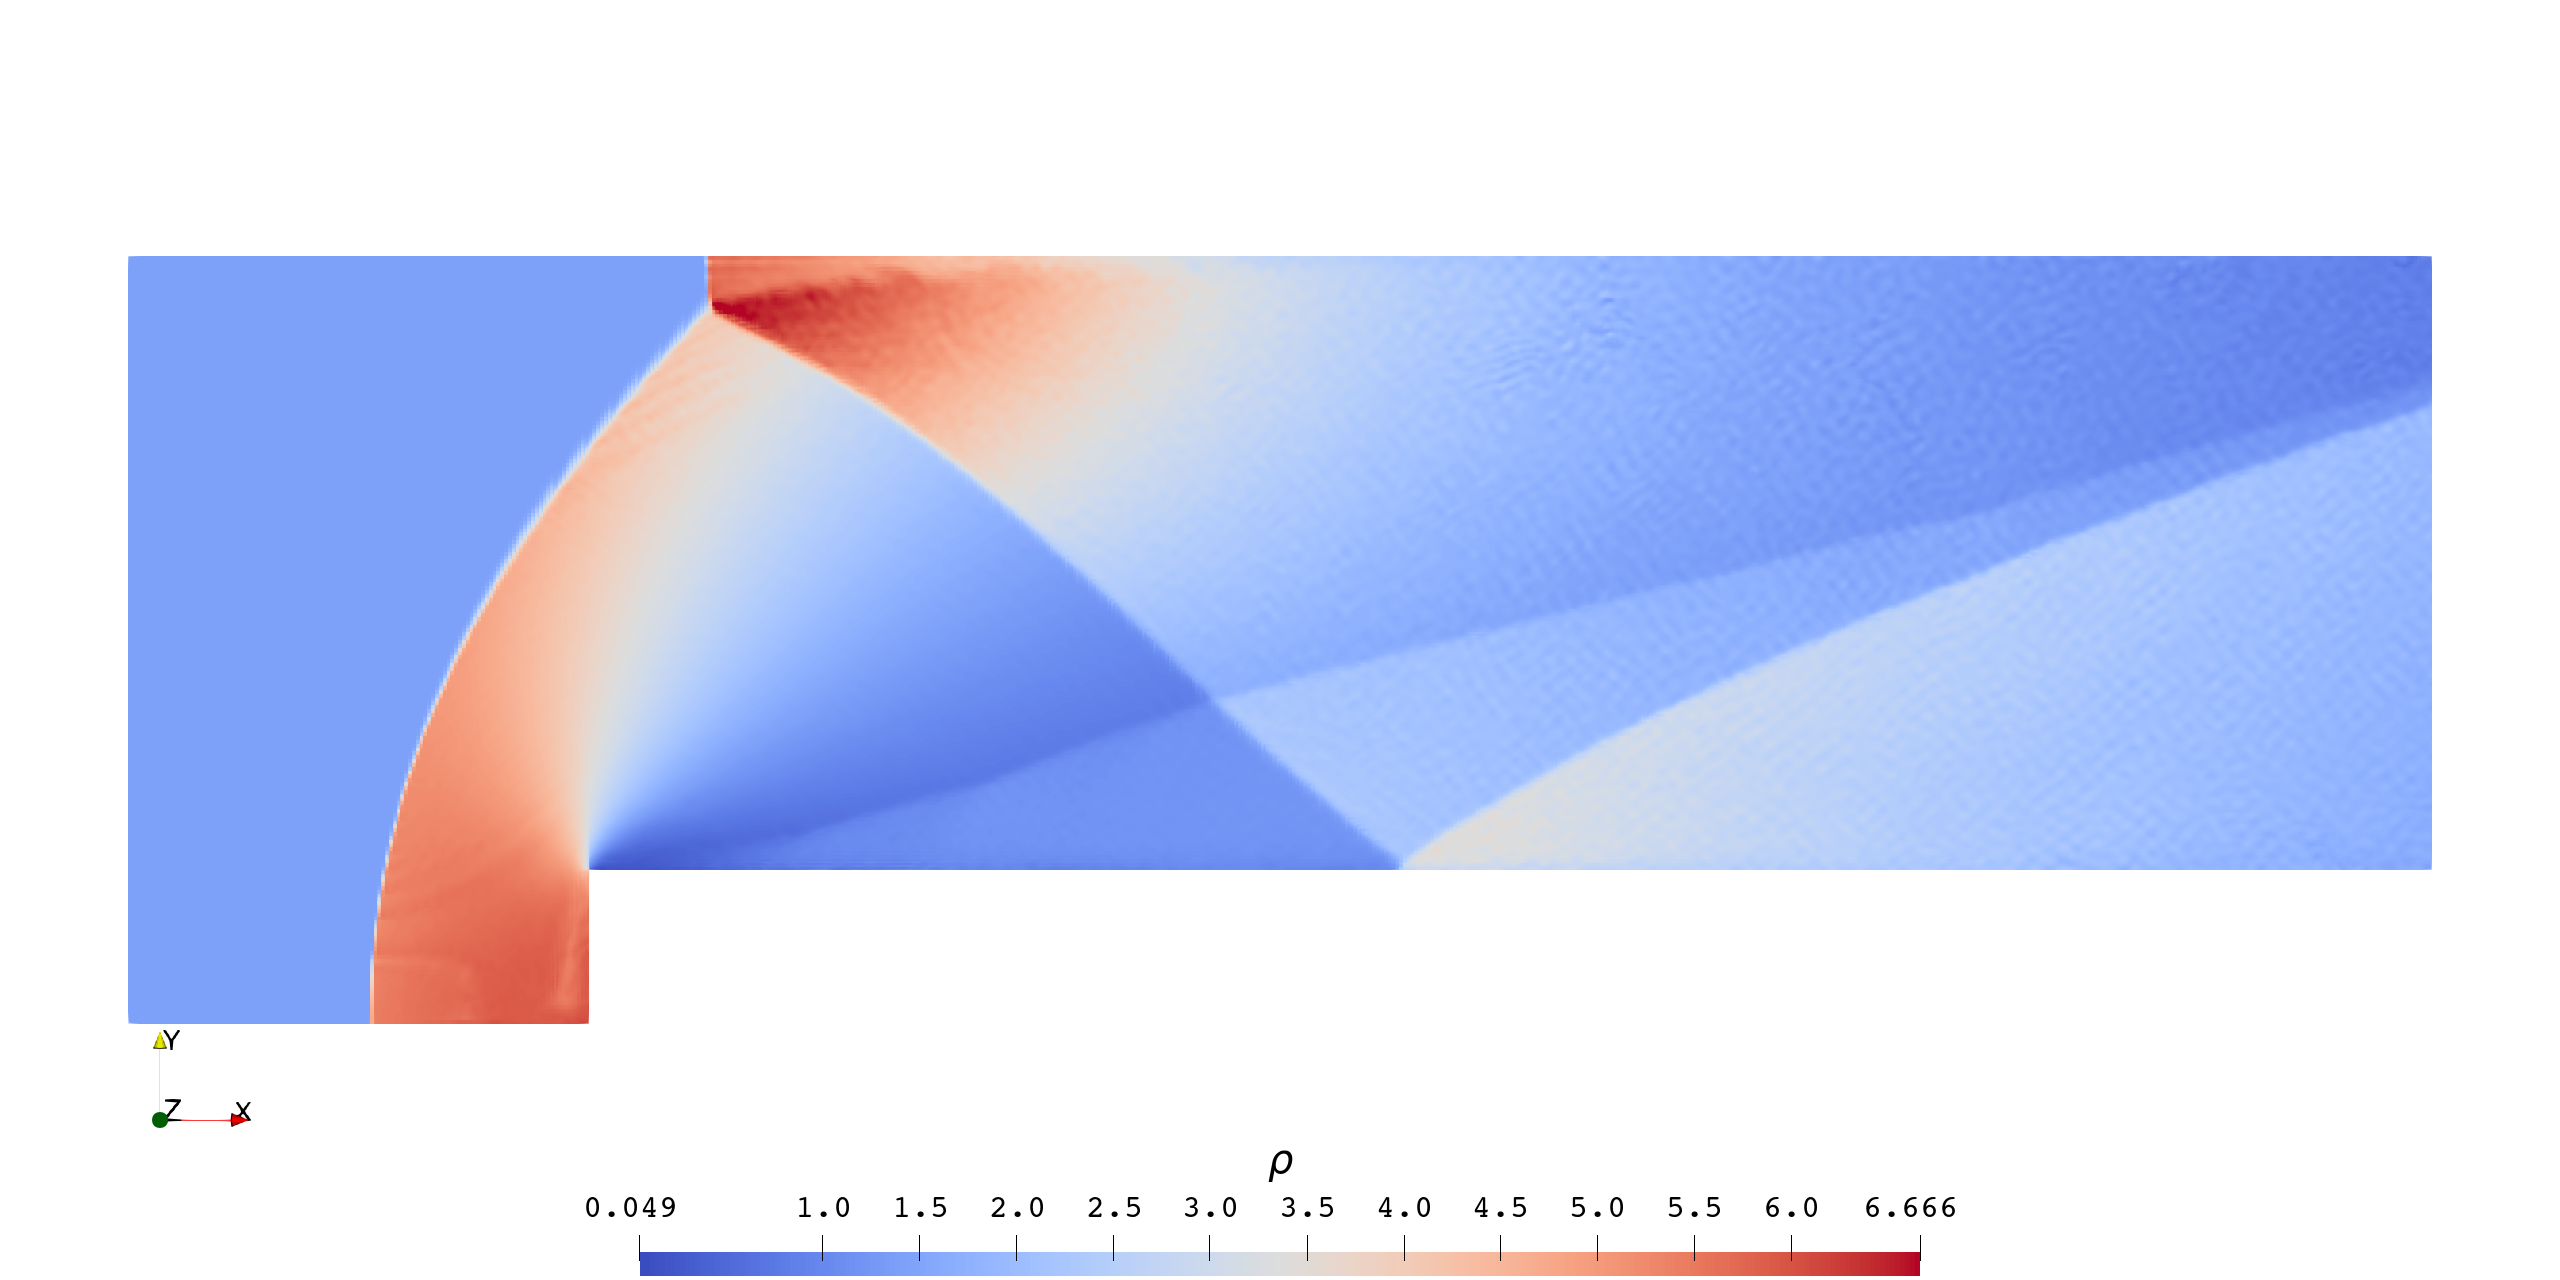
\includegraphics[width=1\textwidth]{figures/forward_step/p=3_t=20e-1}

\caption{\label{fig:forward_step_p=00003D3_t=00003D20e-1}Third-order solution
of Problem \ref{prob:forward_step} at $t=2.0$ on an $h=1/200$ mesh.}
\end{figure}

\begin{figure}
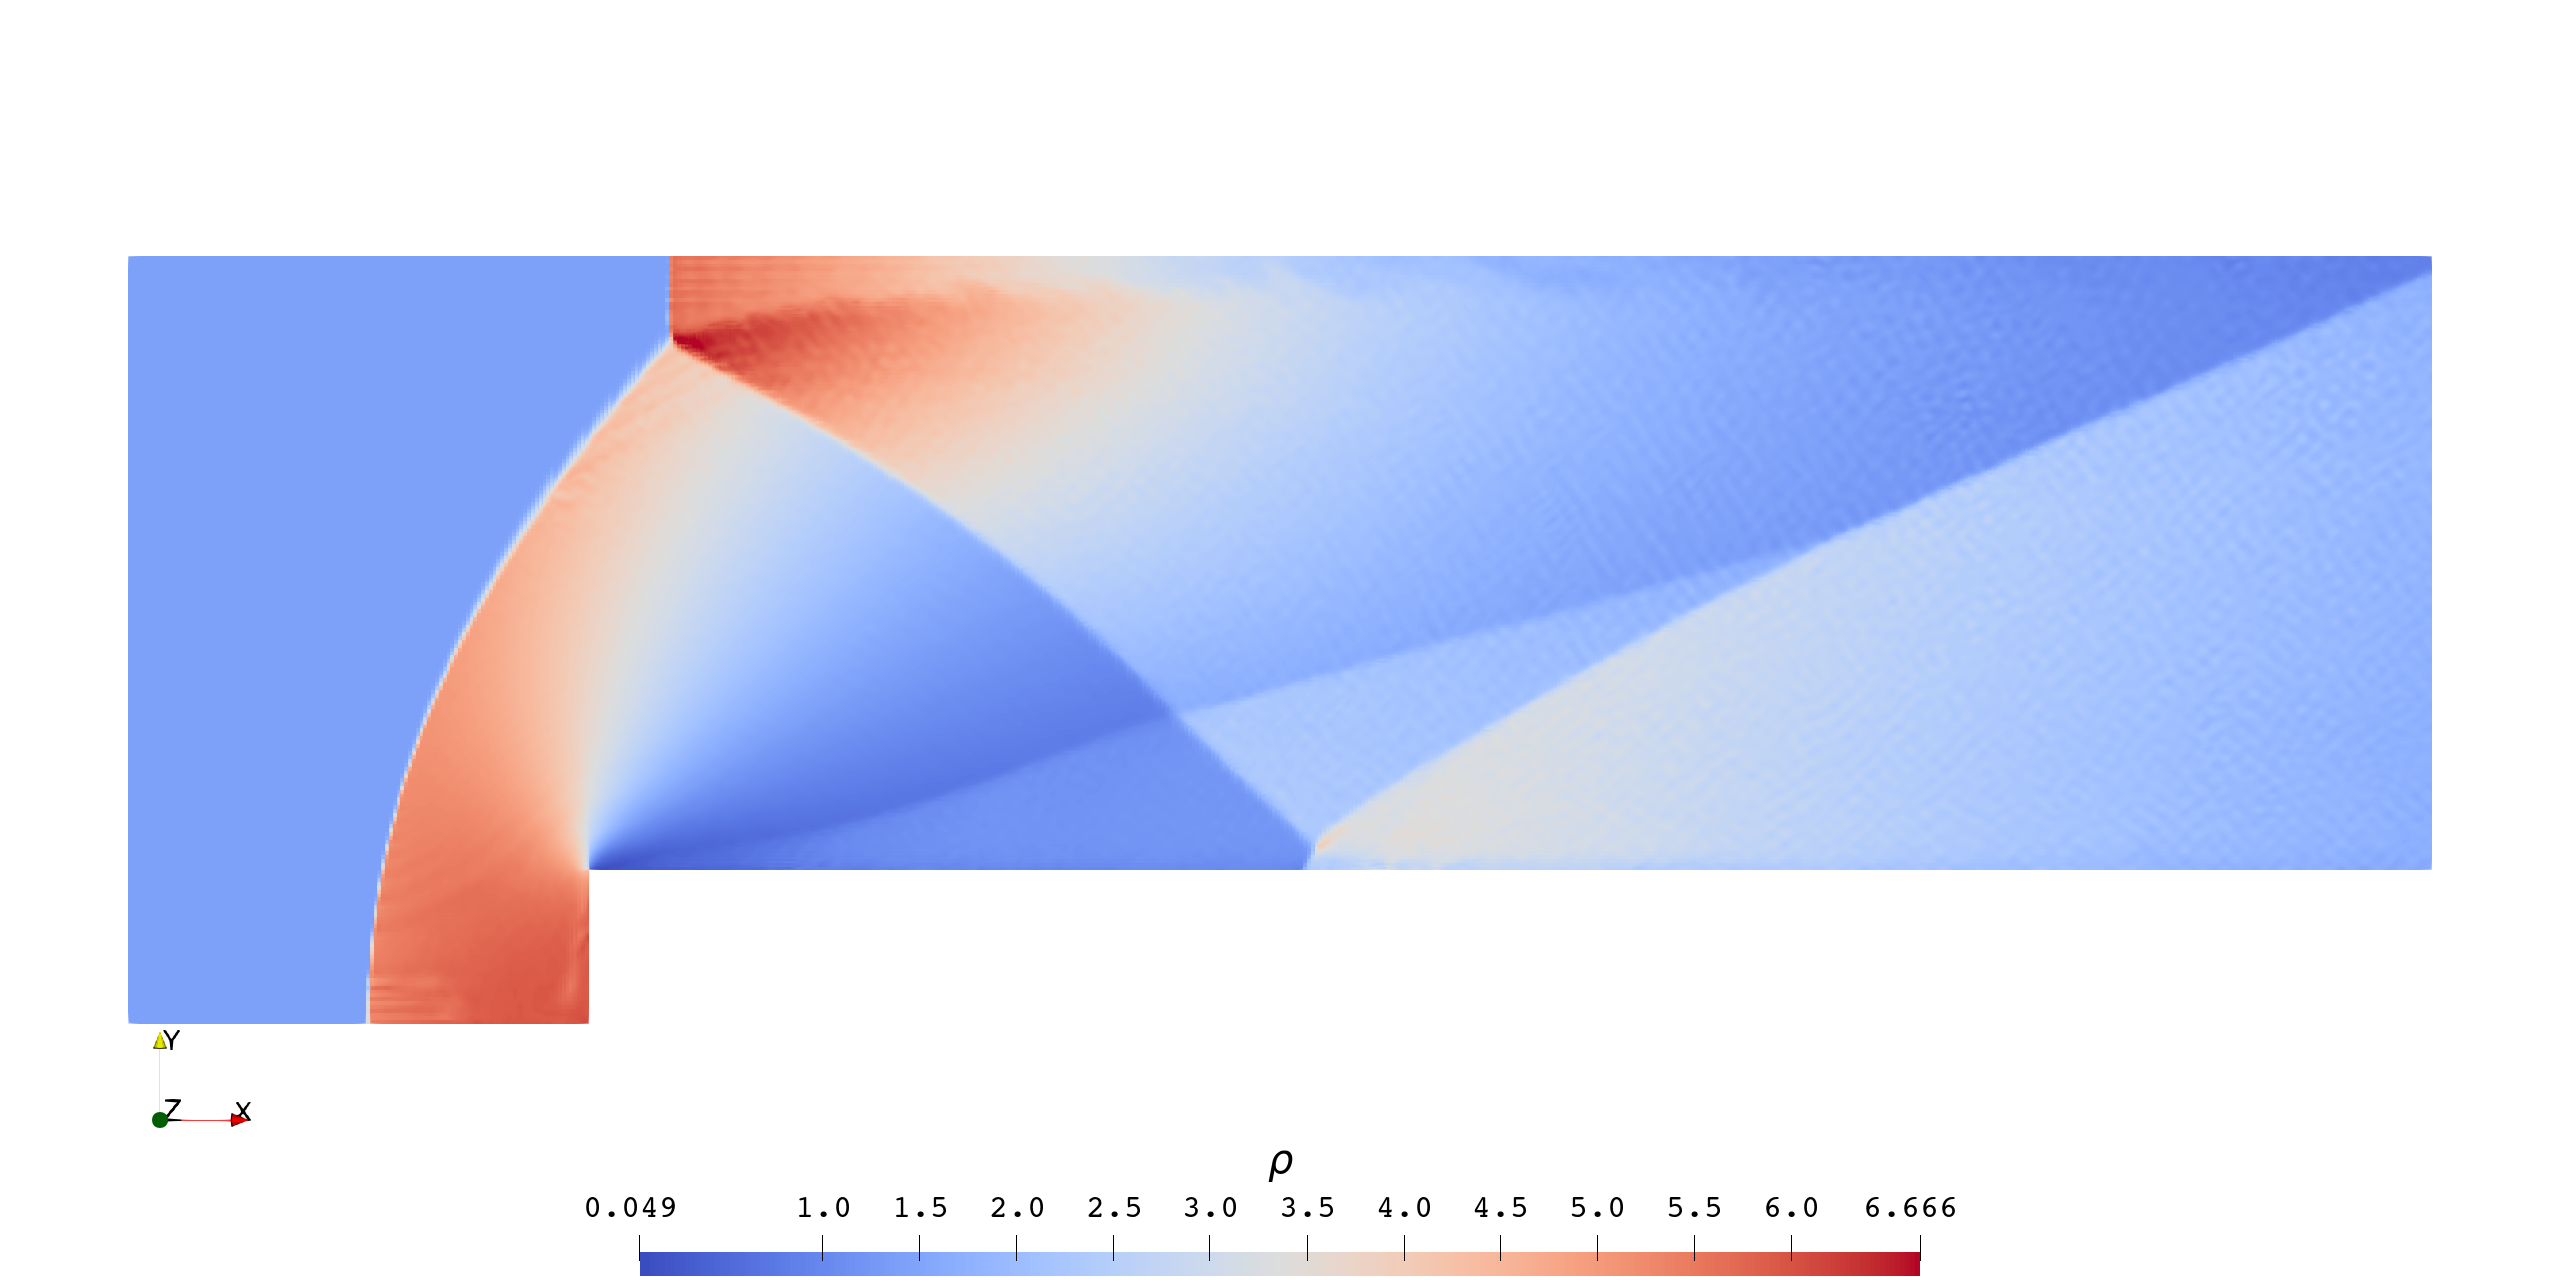
\includegraphics[width=1\textwidth]{figures/forward_step/p=3_t=24e-1}

\caption{\label{fig:forward_step_p=00003D3_t=00003D24e-1}Third-order solution
of Problem \ref{prob:forward_step} at $t=2.4$ on an $h=1/200$ mesh.}
\end{figure}

\begin{figure}
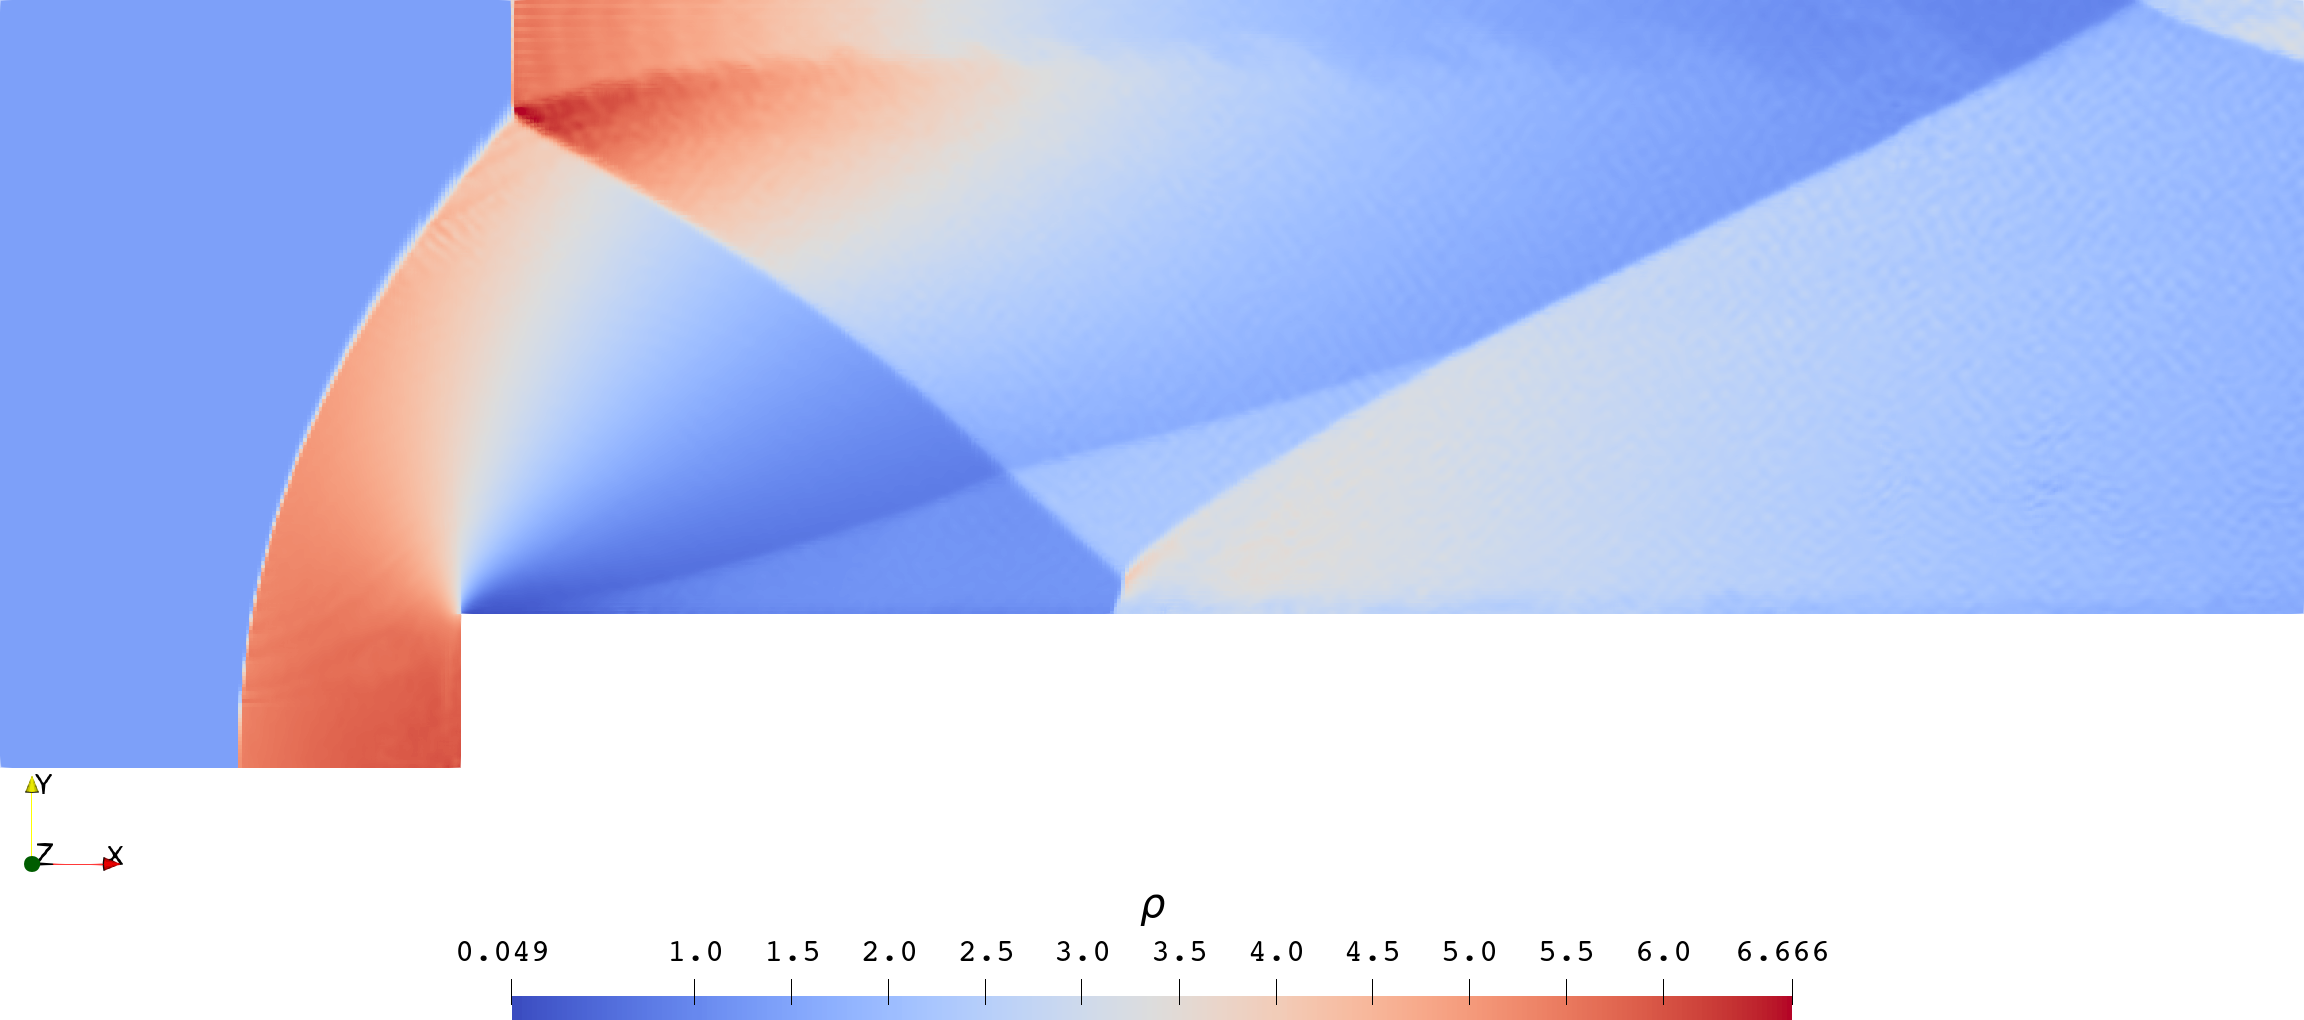
\includegraphics[width=1\textwidth]{figures/forward_step/p=3_t=28e-1}

\caption{\label{fig:forward_step_p=00003D3_h=00003D28e-1}Third-order solution
of Problem \ref{prob:forward_step} at $t=2.8$ on an $h=1/200$ mesh.}
\end{figure}

\begin{figure}
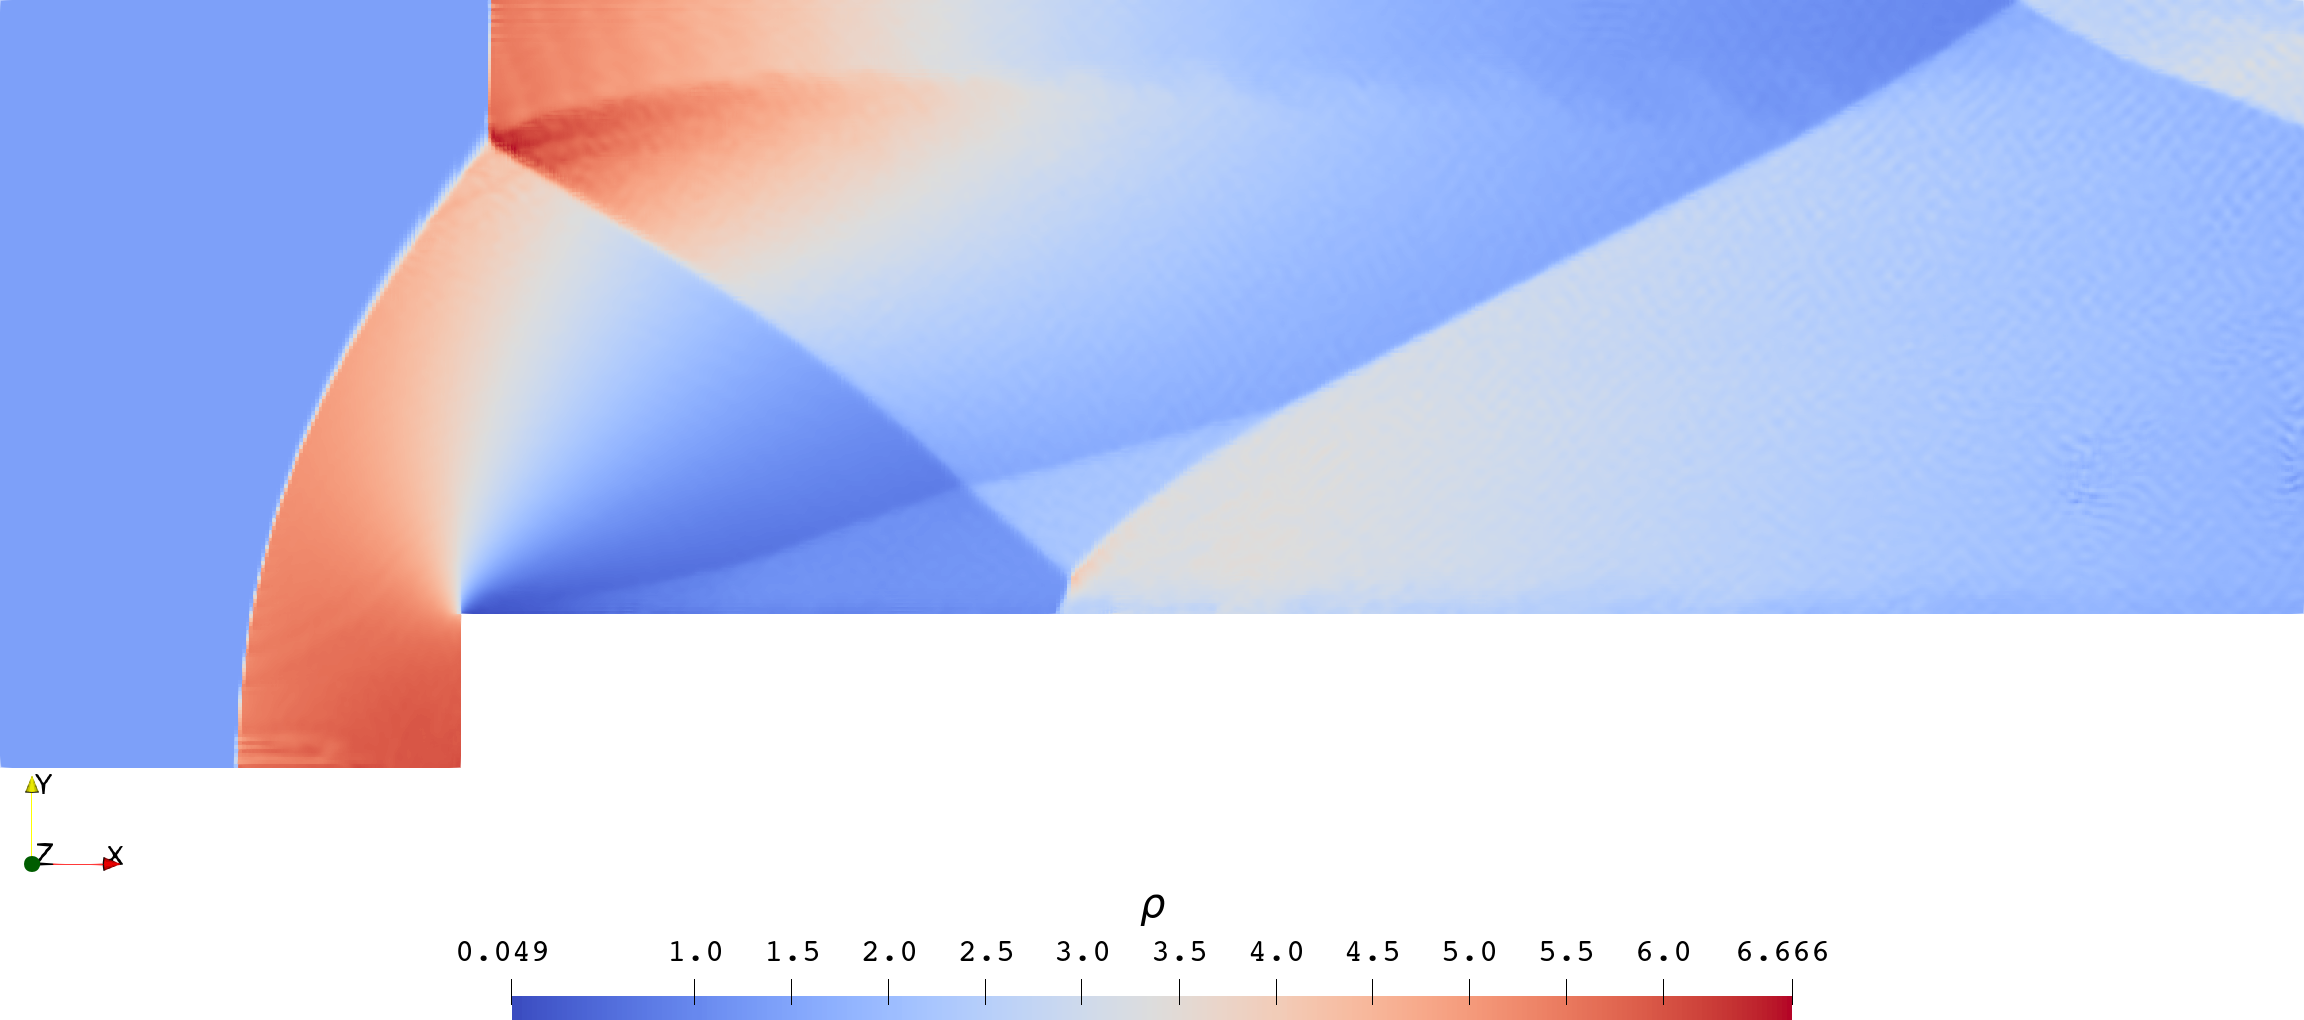
\includegraphics[width=1\textwidth]{figures/forward_step/p=3_t=32e-1}

\caption{\label{fig:forward_step_p=00003D3_t=00003D32e-1}Third-order solution
of Problem \ref{prob:forward_step} at $t=3.2$ on an $h=1/200$ mesh.}
\end{figure}

\begin{figure}
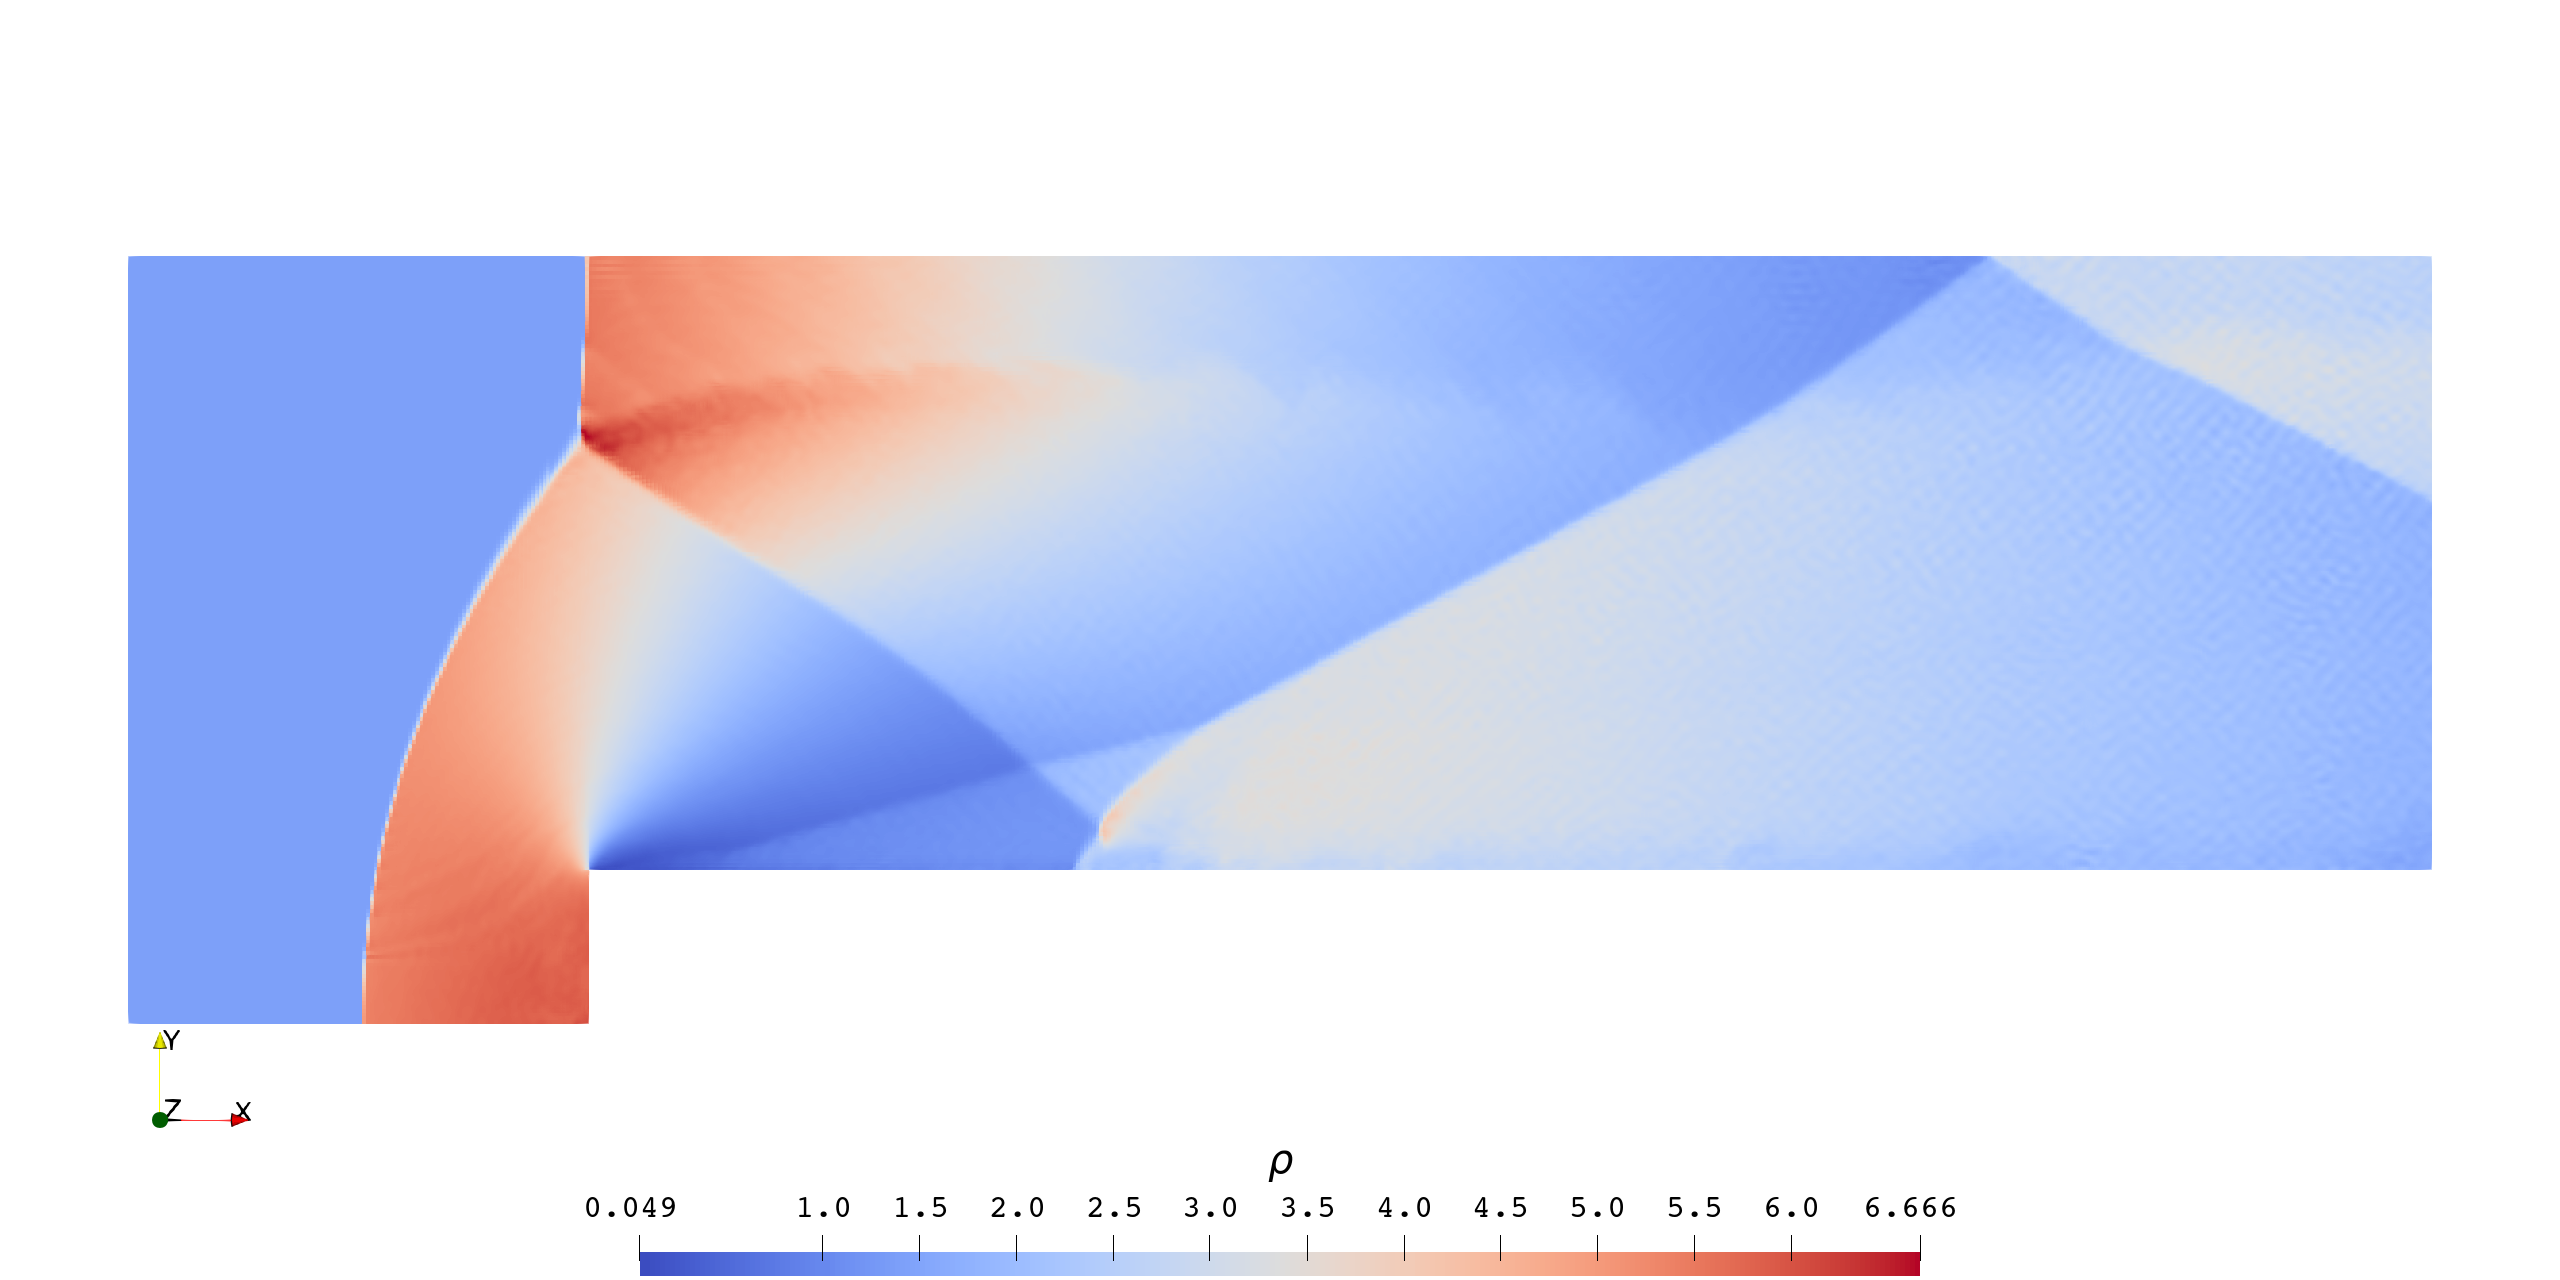
\includegraphics[width=1\textwidth]{figures/forward_step/p=3_t=40e-1}

\caption{\label{fig:forward_step_p=00003D3_t=00003D40e-1}Third-order solution
of Problem \ref{prob:forward_step} at $t=4.0$ on an $h=1/200$ mesh.}
\end{figure}

The flow starts from a uniform supersonic ($M=3.0$) state. In Figures
\ref{fig:forward_step_p=00003D3_t=00003D02e-1} and \ref{fig:forward_step_p=00003D3_t=00003D04e-1},
a curved bow shock wave generates in front of the forward-facing step
and a fan-shaped expansion wave generates at the corner ($x=0.6,y=0.2$).
The bow shock then hits the top of the tunnel (Figure \ref{fig:forward_step_p=00003D3_t=00003D06e-1})
and reflects from it (Figures \ref{fig:forward_step_p=00003D3_t=00003D08e-1}
and \ref{fig:forward_step_p=00003D3_t=00003D10e-1}). At about $t=1.2$
(Figure \ref{fig:forward_step_p=00003D3_t=00003D12e-1}), the reflected
shock hits the bottom of the tunnel (the top of the step) and reflects
from it. Both of the two reflections are regular at these moments.
Just before $t=2.0$ (Figure \ref{fig:forward_step_p=00003D3_t=00003D12e-1}),
a Mach stem which characterizes a Mach reflection has generated from
the first reflection point. A wavy contact discontinuity generating
from the triple point is captured by Figures \ref{fig:forward_step_p=00003D3_t=00003D24e-1}--\ref{fig:forward_step_p=00003D3_t=00003D40e-1}.
This flow structure would be smeared off if we solved Problem \ref{prob:forward_step}
using lower-order solvers or coarser meshes.

\subsection{Three-Dimensional Engineering Problems\label{subsec:YF-17}}

In this section, we solve the Euler system (Equation \ref{eq:euler_system})
on a three-dimensional unstructured mesh, which discretizes the space
around a YF-17 aircraft by tetrahedral cells as shown in Figure \ref{fig:yf17_mesh}.

\begin{figure}
\includegraphics[width=1\textwidth]{figures/yf17/mesh}

\caption{\label{fig:yf17_mesh}A zoomed-in view of the most important boundaries
of the mesh for solving problems in Section \ref{subsec:YF-17}.}
\end{figure}


\subsubsection{YF-17 in Subsonic Flight}
\begin{Problem}
\label{prob:Subsonic-YF17}Solve the Euler system (Equation \ref{eq:euler_system})
in the surrounding of a YF-17 aircraft. The initial condition is given
as a subsonic flow ($M=0.3$) with a $20$-deg angle of attack:

\[
\begin{bmatrix}\rho & u & v & w & p\end{bmatrix}_{t=0}=\begin{bmatrix}1.4 & 0.2819 & 0.0 & 0.1026 & 1.0\end{bmatrix}.
\]

All boundaries of the aircraft are defined as solid walls, except
the intake the engine which is defined as a subsonic outlet of the
condition equal to the initial condition, and the exhaust of the engine
which is defined as a supersonic ($M=3.0$) inlet of the condition:

\[
\begin{bmatrix}\rho & u & v & w & p\end{bmatrix}_{\text{ex.}}=\begin{bmatrix}1.4 & 2.4 & 0.0 & 0.0 & 1.44\end{bmatrix}.
\]
\end{Problem}

\begin{figure}
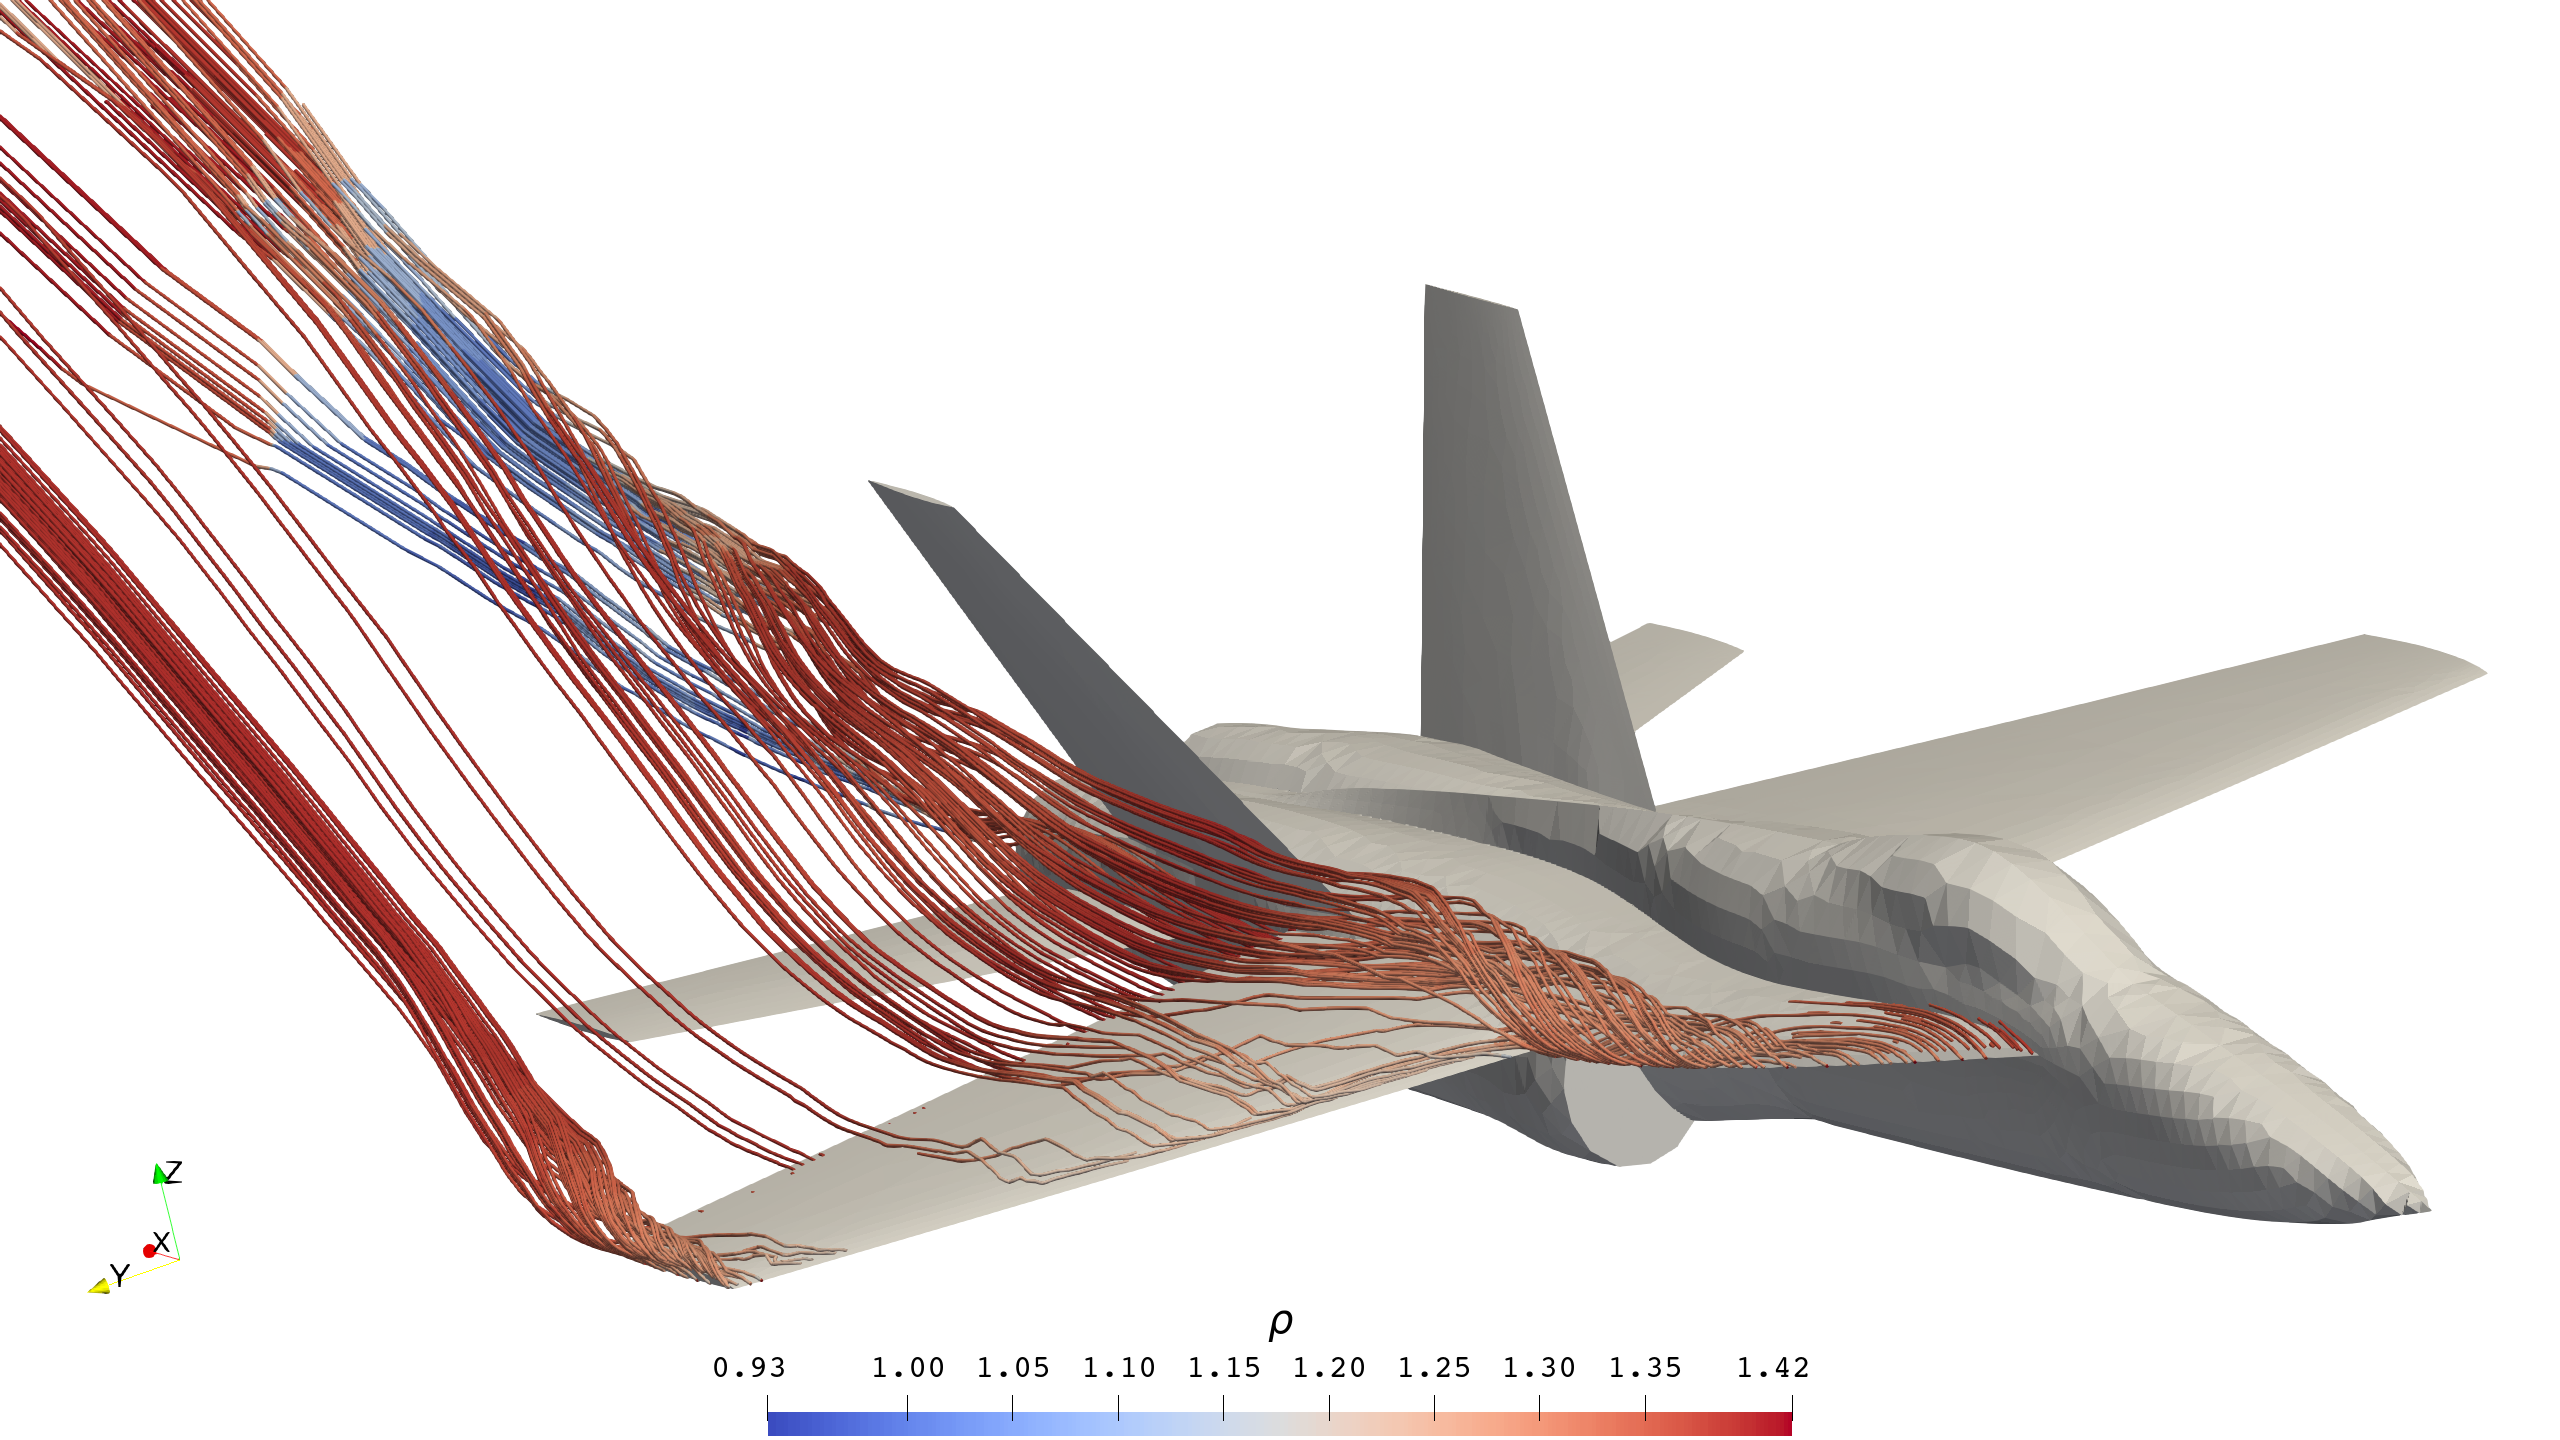
\includegraphics[width=1\textwidth]{figures/yf17/streamlines_p=1}

\caption{\label{fig:yf17_streamlines_p=00003D1}Streamlines given by the first-order
solution of Problem \ref{prob:Subsonic-YF17}.}
\end{figure}

\begin{figure}
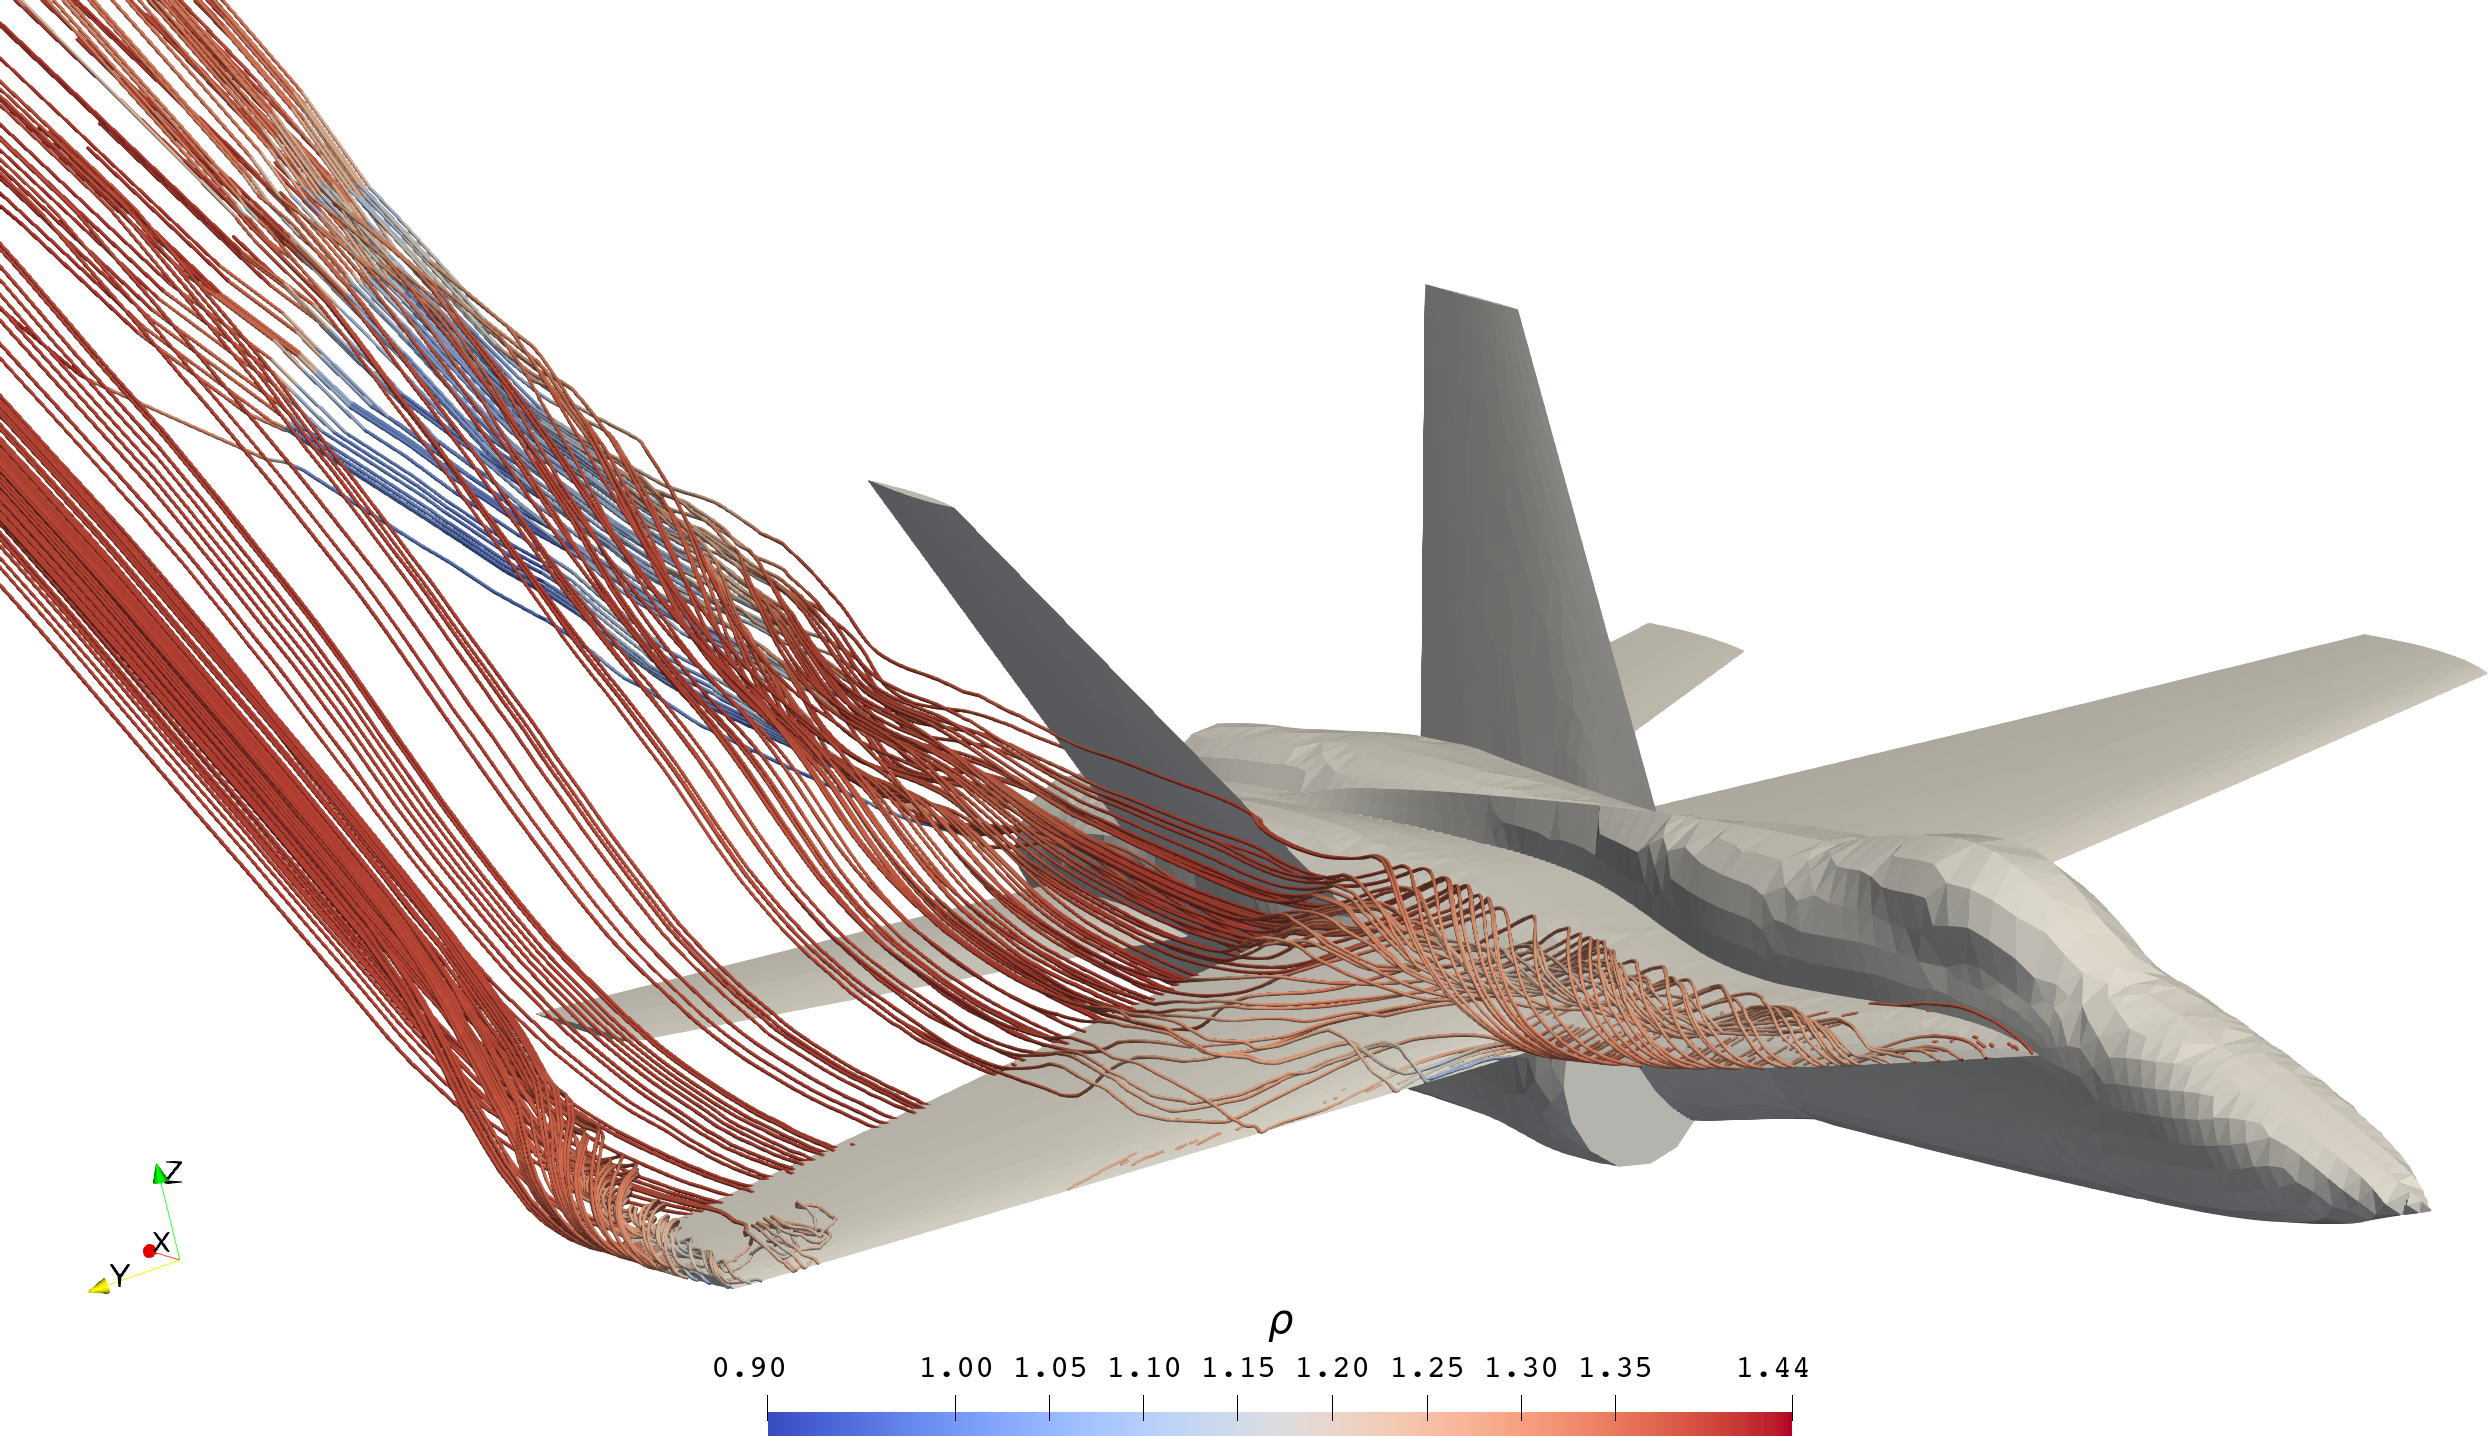
\includegraphics[width=1\textwidth]{figures/yf17/streamlines_p=3}

\caption{\label{fig:yf17_streamlines_p=00003D3}Streamlines given by the third-order
solution of Problem \ref{prob:Subsonic-YF17}.}
\end{figure}

We solve this problem by two of our finite element solvers and plot
the streamlines released from the strake and the wing at $t=10$ in
Figure \ref{fig:yf17_streamlines_p=00003D1} and Figure \ref{fig:yf17_streamlines_p=00003D3}.
It can be seen that the streamlines obtained from the high-order ($p=3$)
solution are smoother than those from the low-order ($p=1$) solution,
which shows the benefit of $p$-refinement. The difference in accuracy
is more obvious in Figure \ref{fig:yf17_rho_subsonic}, which clearly
shows a more detailed flow structure in the third-order solution (left
half) and the piecewise constantness of the first-order solution (right
half). Both solutions are able to capture the vortex trailing from
the wing tip, which is generated from the the pressure difference
between the upper and lower surfaces of the wing. When the wing generates
positive lift, the pressure on the lower wing surface is higher than
that on the upper wing surface. Under the action of this pressure
difference, the air under the wing rolls up around the tip and flows
backward, the tip vortex is thus formed. The vortex trailing from
the strake is generated from a similar mechanism.

\begin{figure}
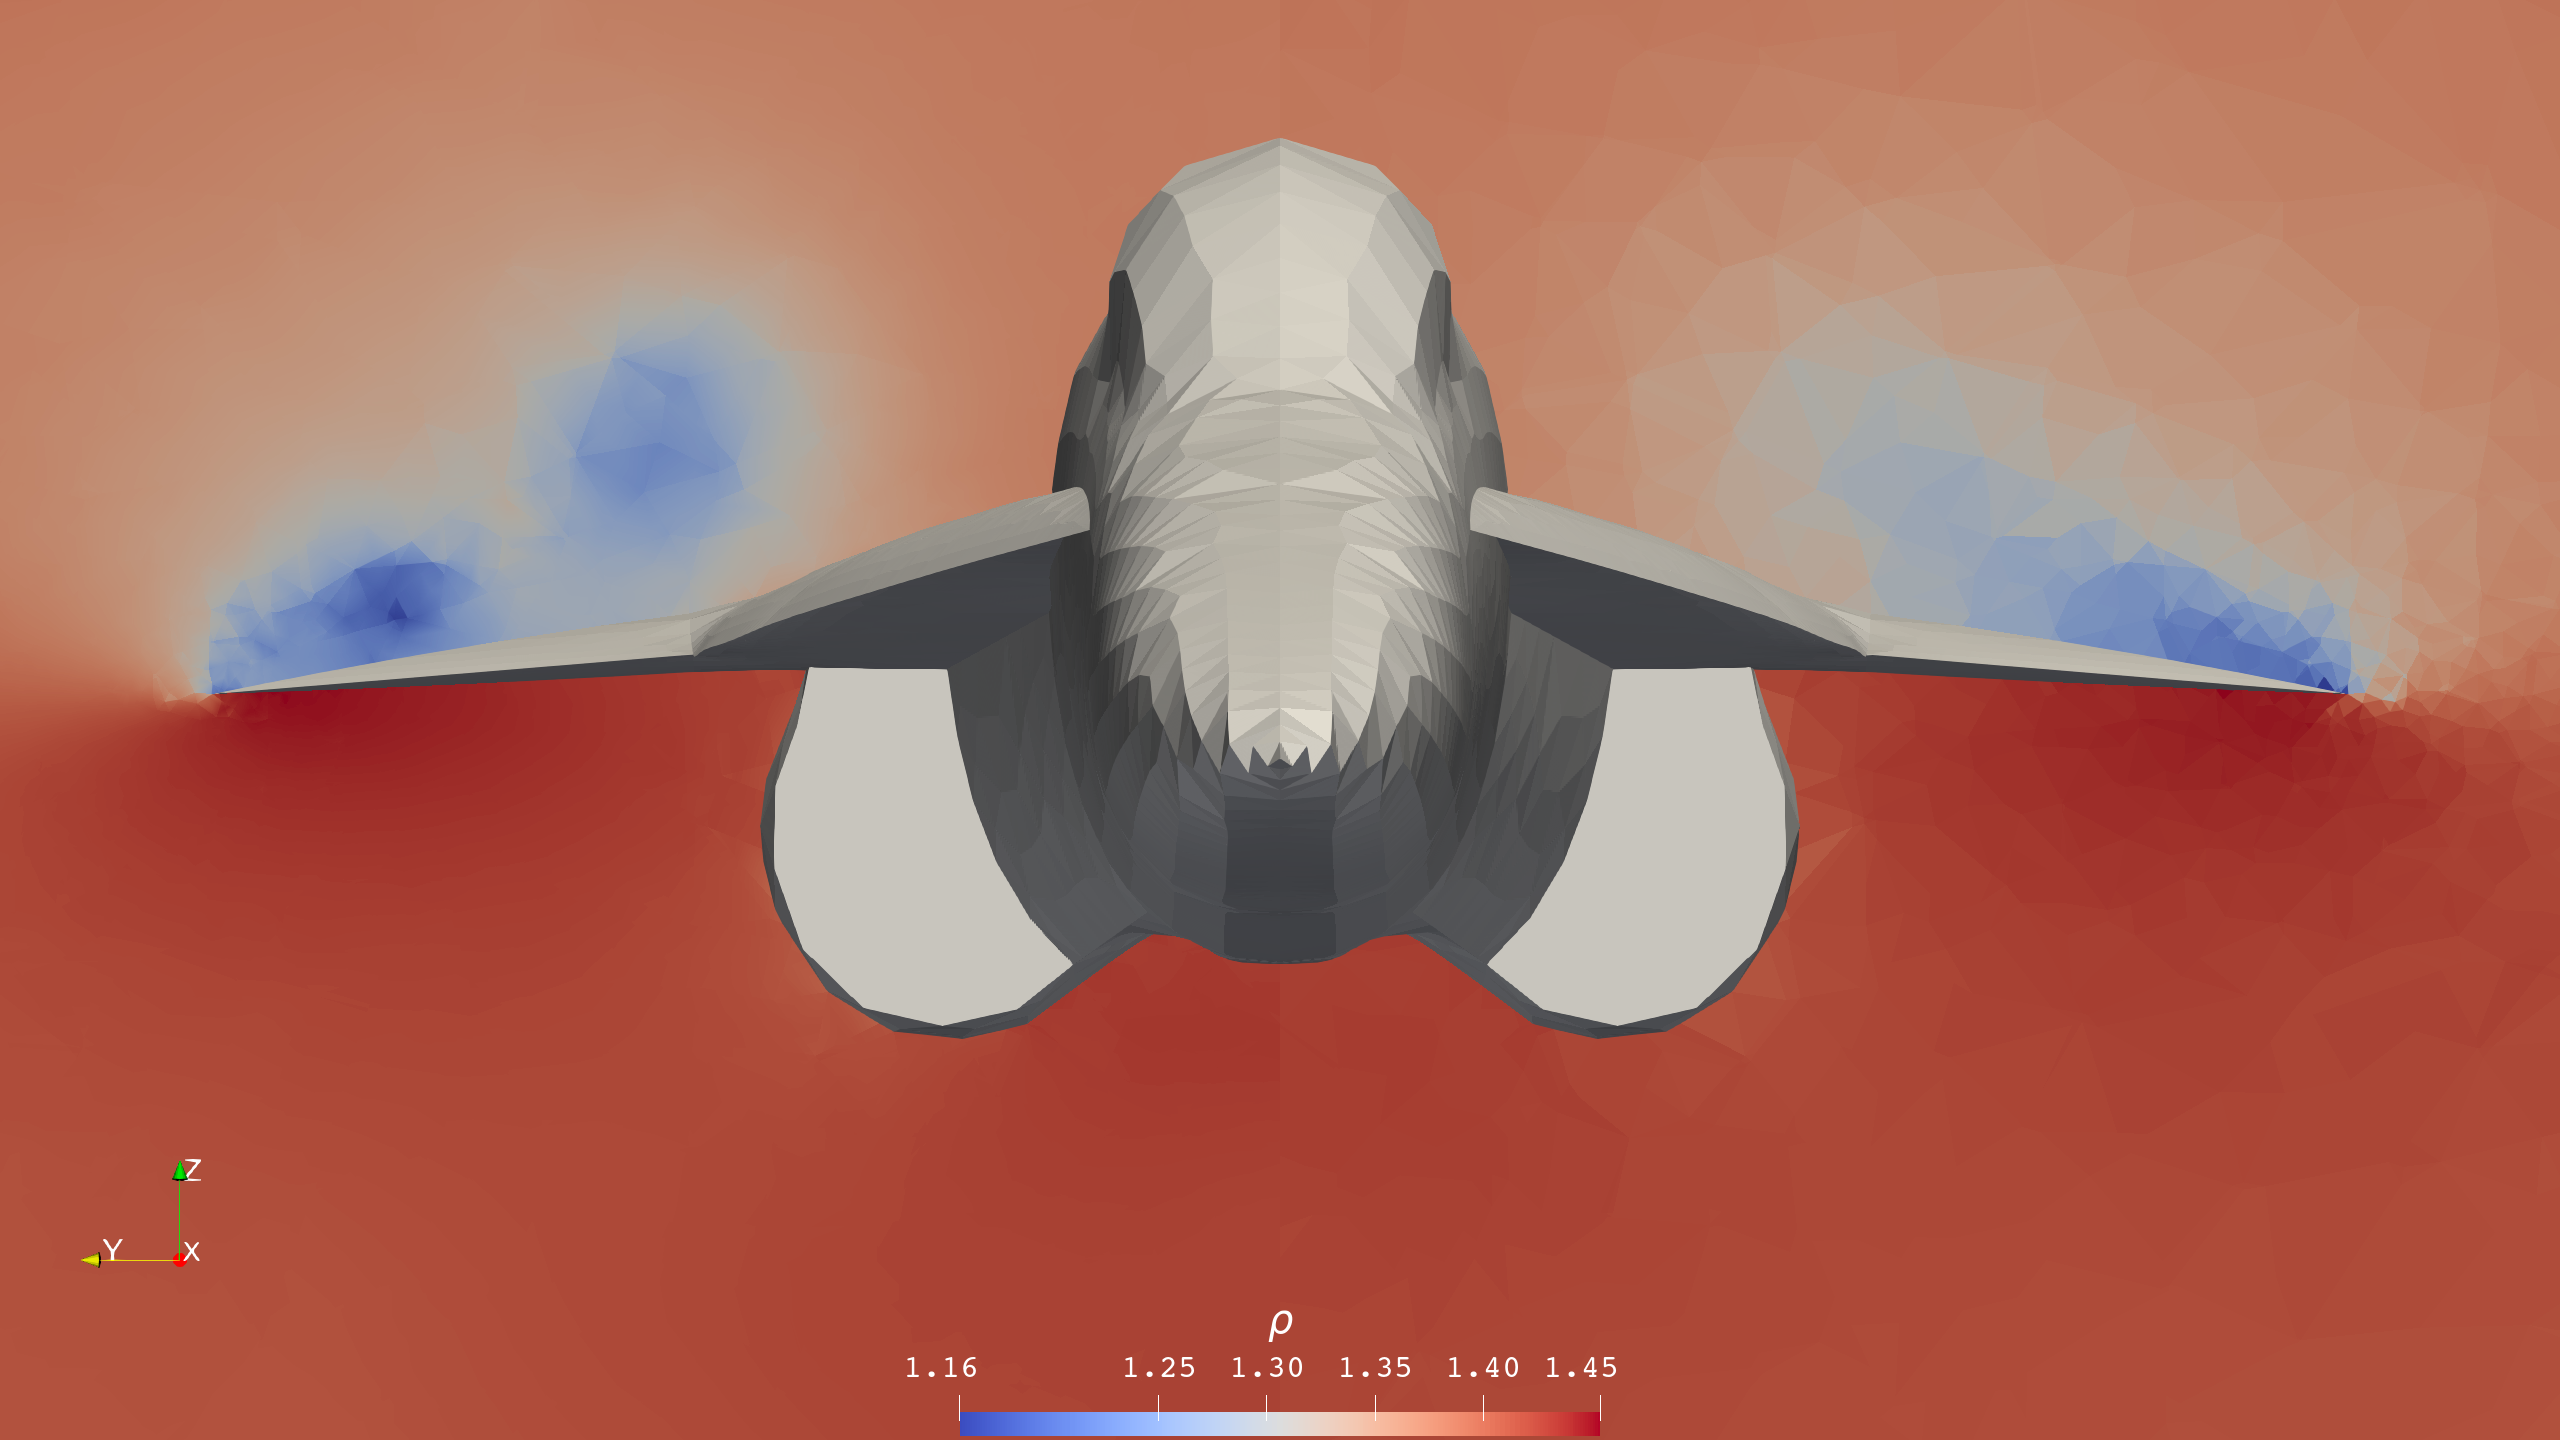
\includegraphics[width=1\textwidth]{figures/yf17/rho_subsonic}

\caption{\label{fig:yf17_rho_subsonic}Comparison between the third-order solution
(left half) and the first-order solution (right half) of Problem \ref{prob:Subsonic-YF17}.}
\end{figure}


\subsubsection{YF-17 in Supersonic Flight}
\begin{Problem}
\label{prob:Supersonic-YF17}Solve the Euler system (Equation \ref{eq:euler_system})
in the surrounding of a YF-17 aircraft. The initial condition is given
as a supersonic flow ($M=2.0$) with a $0$-deg angle of attack:

\[
\begin{bmatrix}\rho & u & v & w & p\end{bmatrix}_{t=0}=\begin{bmatrix}1.4 & 2.0 & 0.0 & 0.0 & 1.0\end{bmatrix}.
\]

All boundaries of the aircraft are defined as solid walls, except
the intake the engine which is defined as a supersonic outlet of the
condition equal to the initial condition, and the exhaust of the engine
which is defined as a supersonic ($M=3.0$) inlet of the condition:

\[
\begin{bmatrix}\rho & u & v & w & p\end{bmatrix}_{\text{ex.}}=\begin{bmatrix}1.4 & 2.4 & 0.0 & 0.0 & 1.44\end{bmatrix}.
\]
\end{Problem}

\begin{figure}
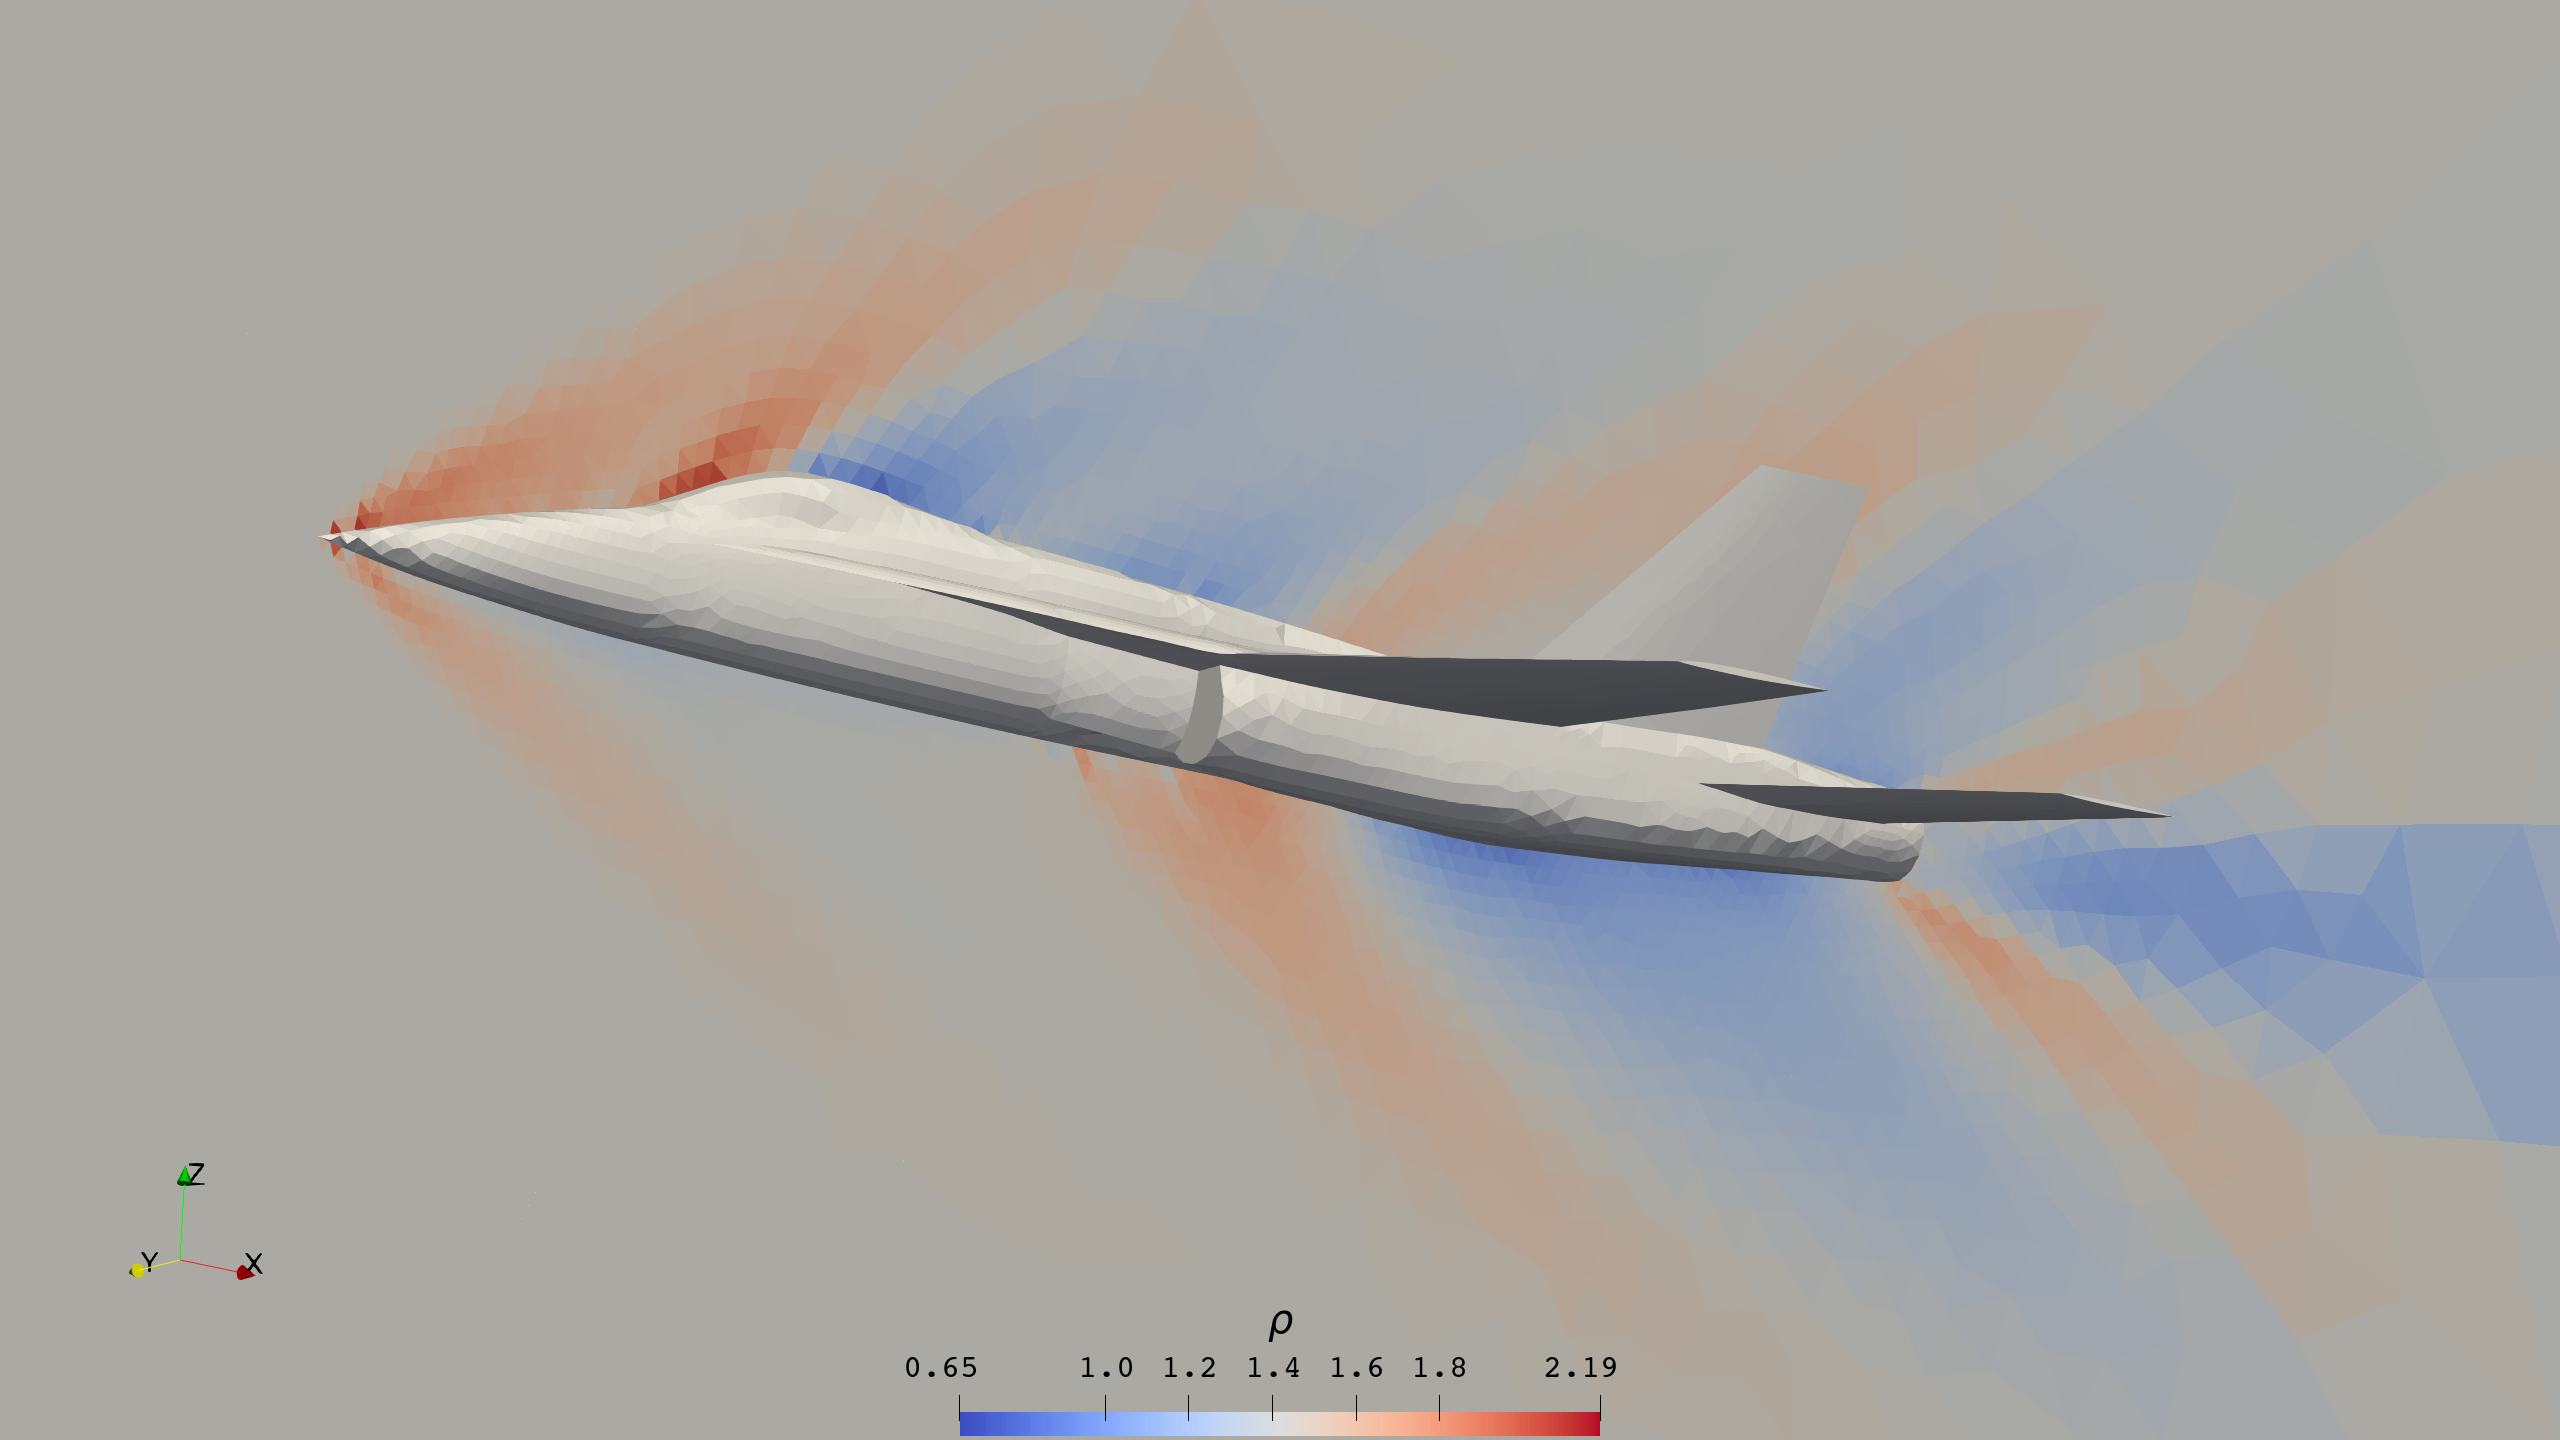
\includegraphics[width=1\textwidth]{figures/yf17/rho_p=1}

\caption{\label{fig:yf17_rho_p=00003D1}Density contour obtained from the first-order
solution of Problem \ref{prob:Supersonic-YF17}.}
\end{figure}

\begin{figure}
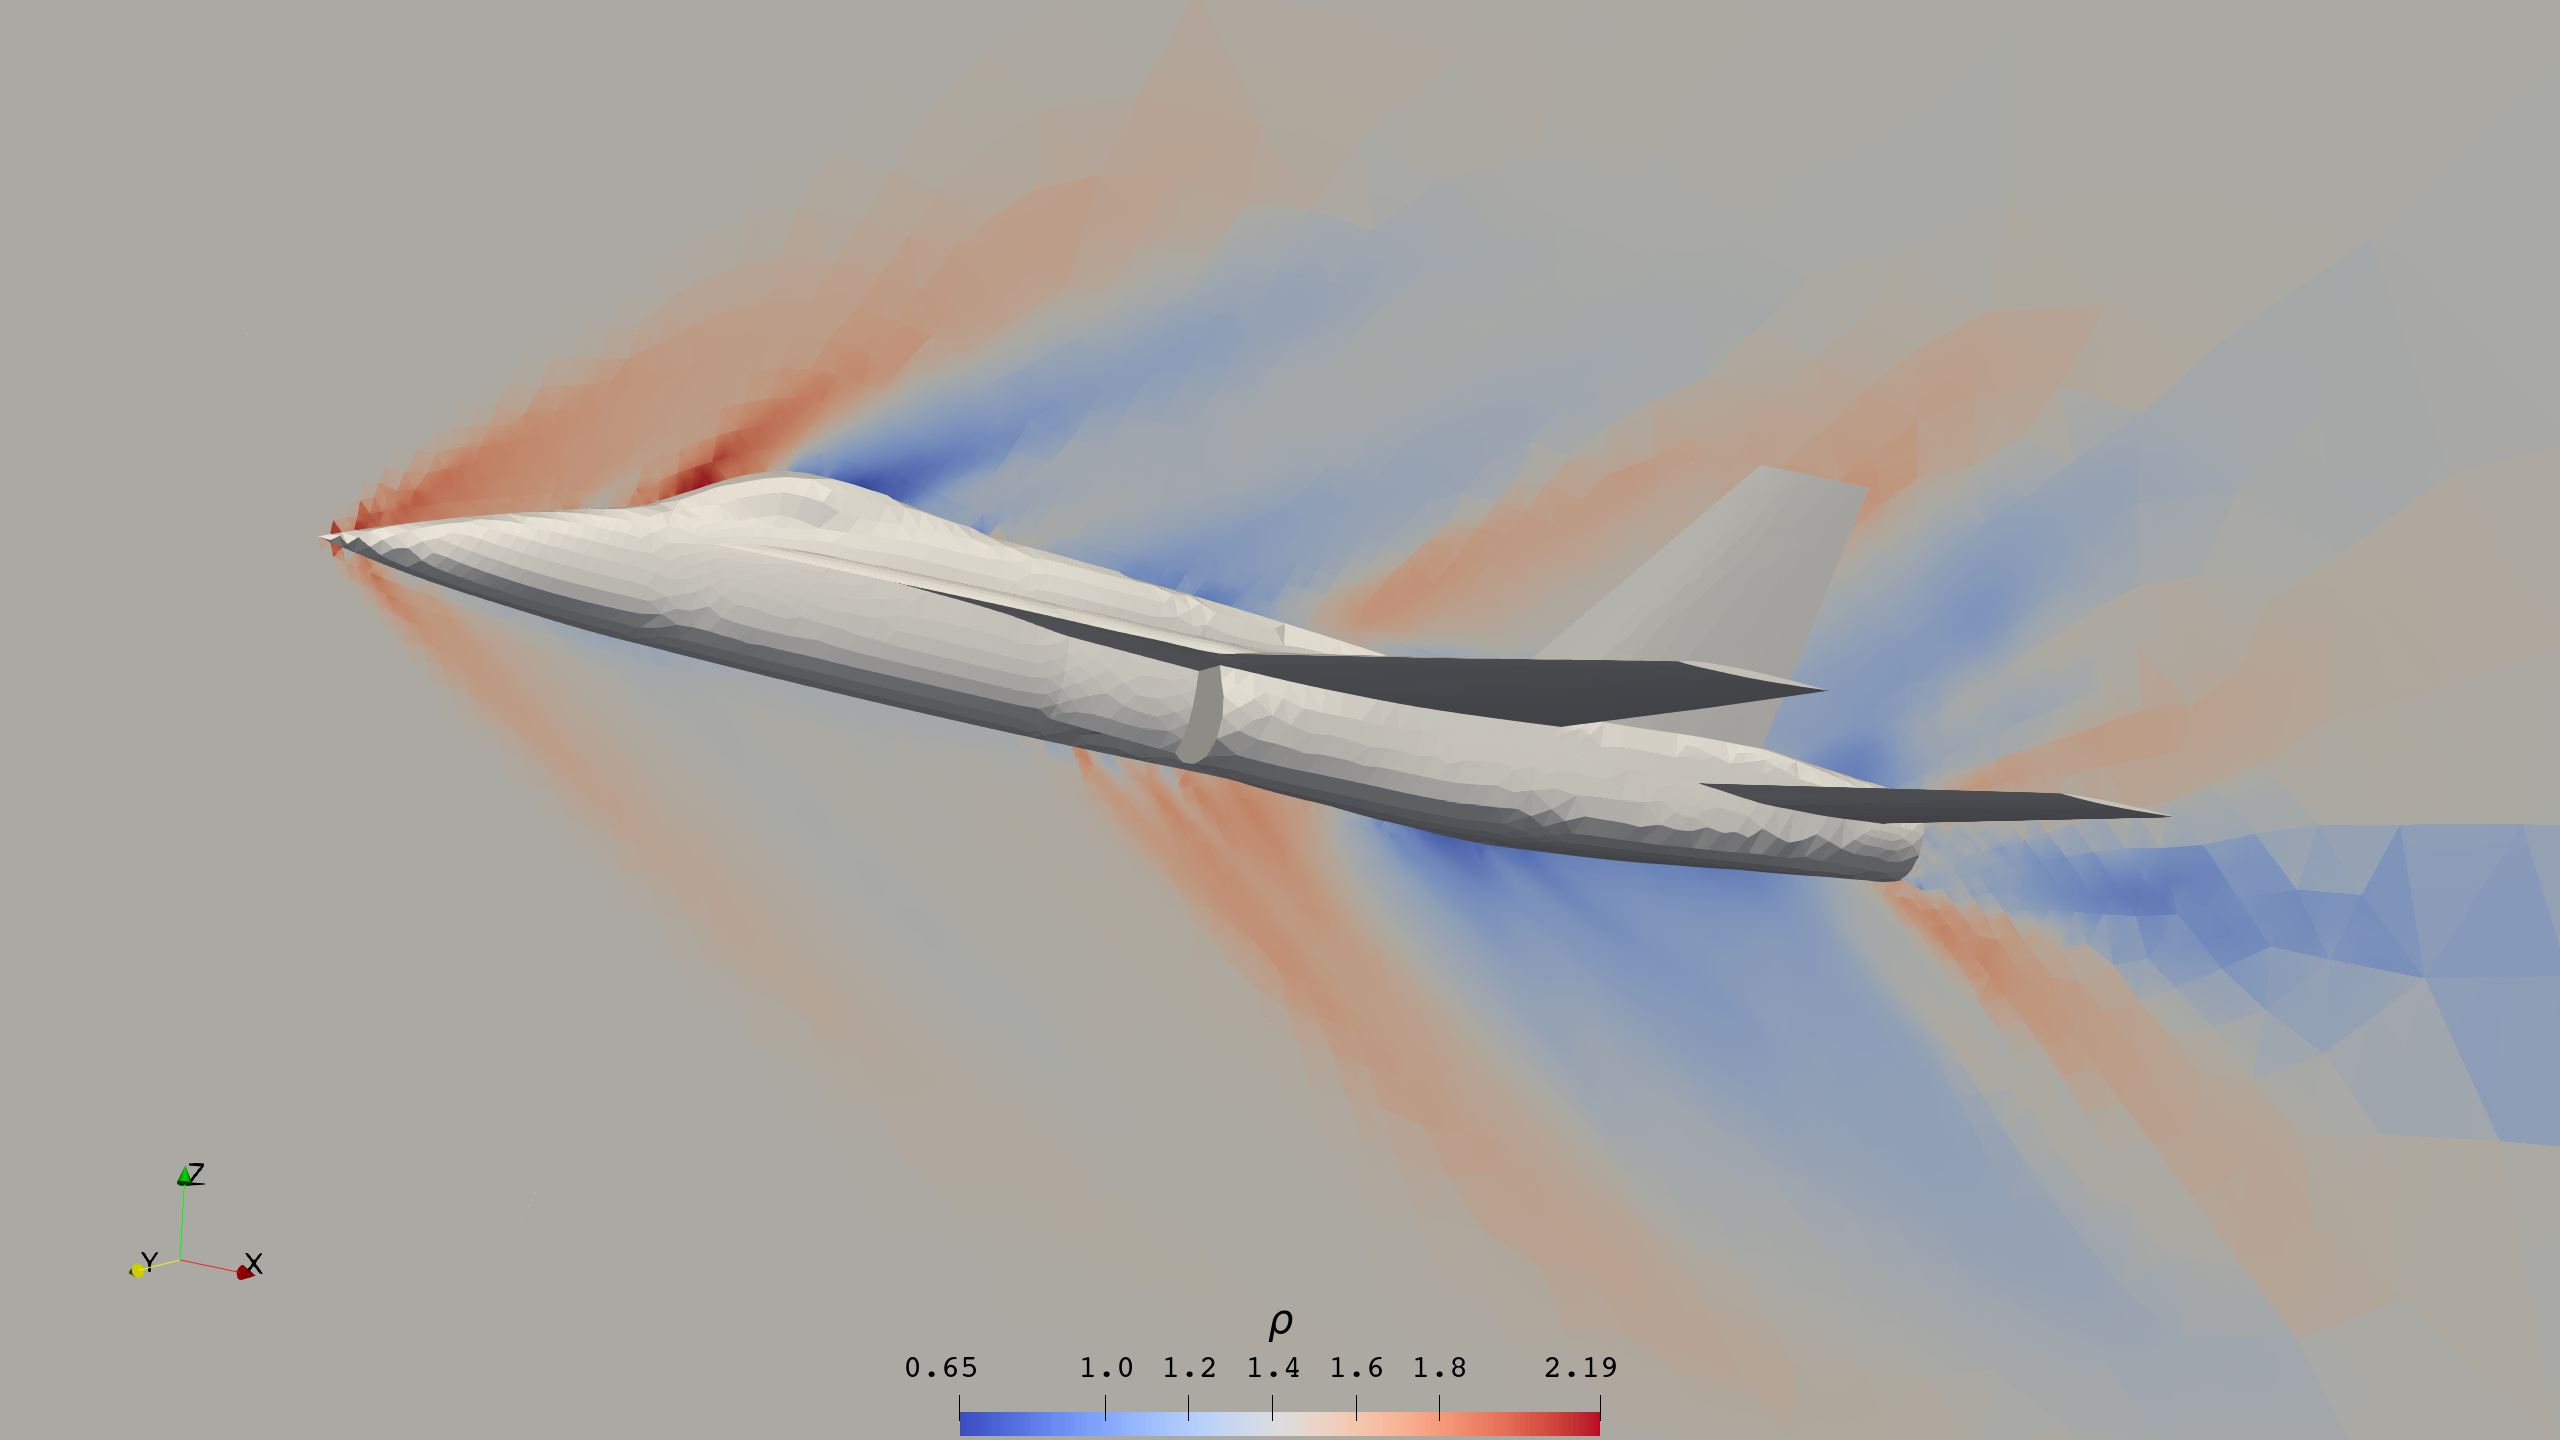
\includegraphics[width=1\textwidth]{figures/yf17/rho_p=3}

\caption{\label{fig:yf17_rho_p=00003D3}Density contour obtained from the third-order
solution of Problem \ref{prob:Supersonic-YF17}.}
\end{figure}

\begin{figure}
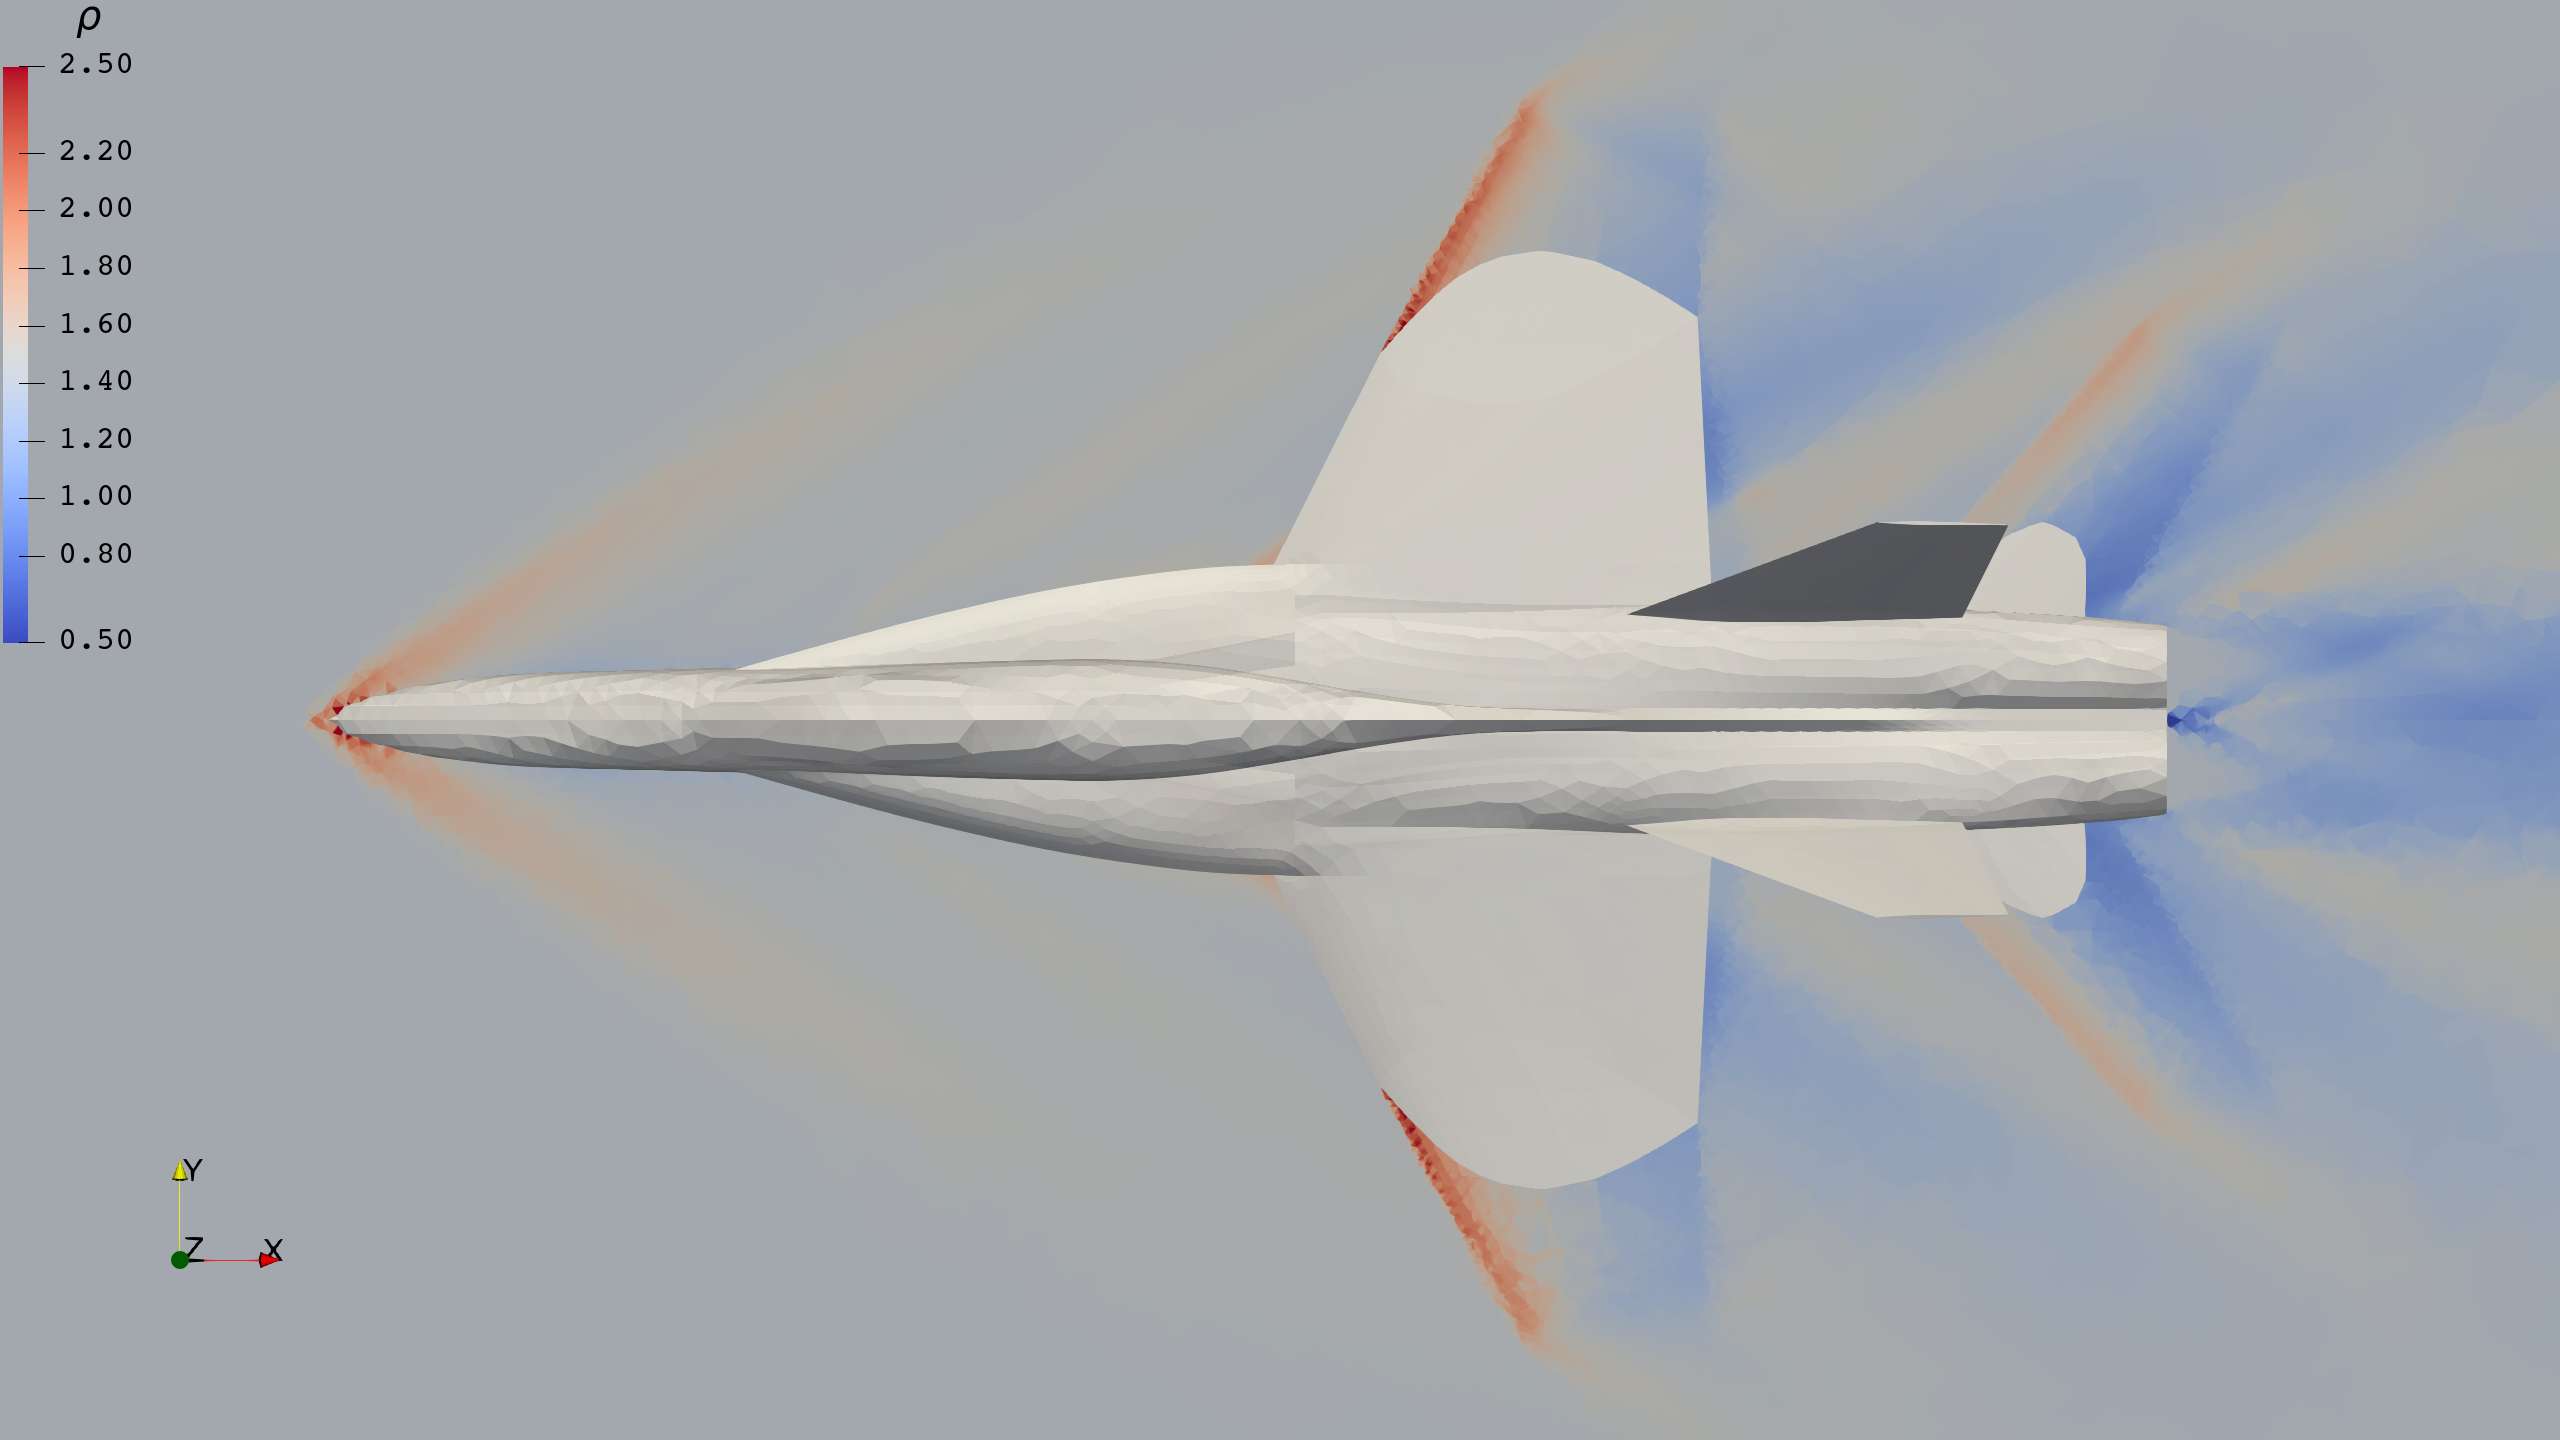
\includegraphics[width=1\textwidth]{figures/yf17/supersonic_top_view}

\caption{\label{fig:yf17_supersonic_top_view}Comparison between the third-order
solution (upper half) and the first-order solution (lower half) of
Problem \ref{prob:Supersonic-YF17} on the $z=0$ surface (top view).}
\end{figure}

\begin{figure}
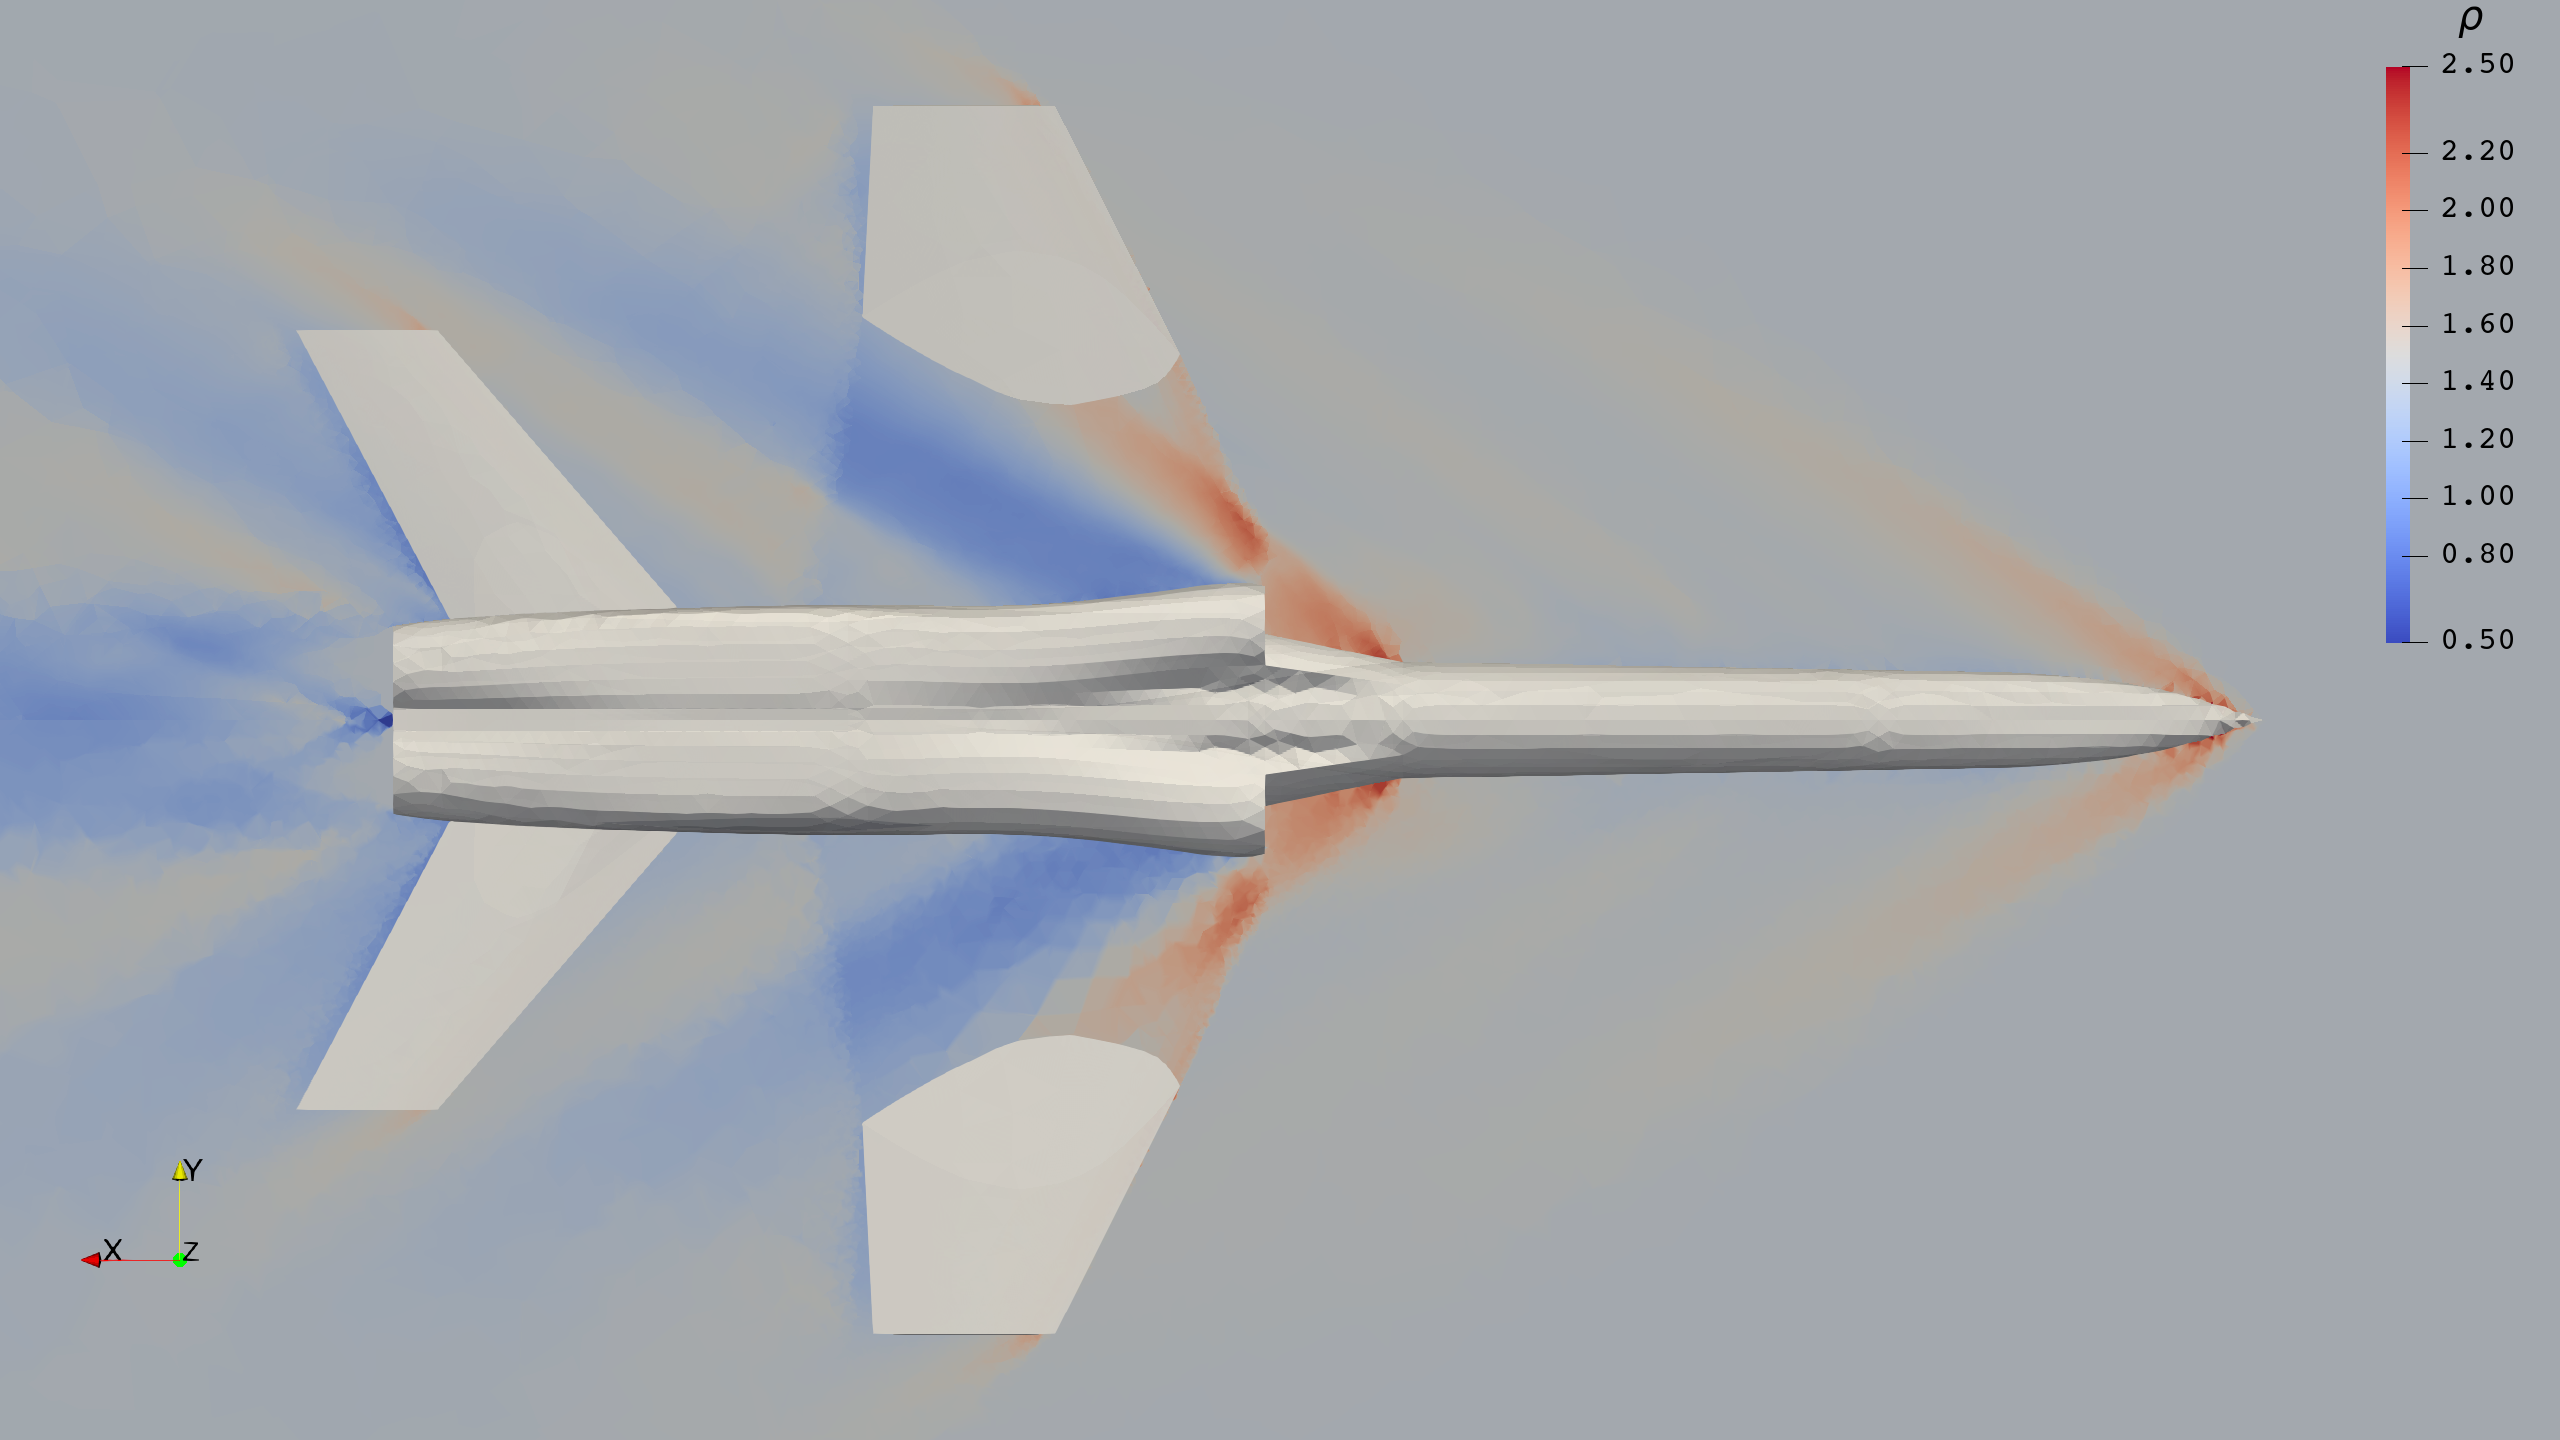
\includegraphics[width=1\textwidth]{figures/yf17/supersonic_bottom_view}

\caption{\label{fig:yf17_supersonic_bottom_view}Comparison between the third-order
solution (upper half) and the first-order solution (lower half) of
Problem \ref{prob:Supersonic-YF17} on the $z=0$ surface (bottom
view).}
\end{figure}

We solve this problem using the same solvers as for Problem \ref{prob:Subsonic-YF17}.
Density contours on the $y=0$ surface obtained from the first- and
the third-order solutions are given in Figure \ref{fig:yf17_rho_p=00003D1}
and Figure \ref{fig:yf17_rho_p=00003D3}, respectively. It is obvious
that shock waves are captured well (without spurious oscillations)
by both of them. To show the difference more clearly, we compare the
two solutions in Figure \ref{fig:yf17_supersonic_top_view} and Figure
\ref{fig:yf17_supersonic_bottom_view}. As in the subsonic case, the
third-order solution (which is piecewise quadratic) outperforms the
first-order one (which is piecewise constant). Shock waves (red) are
generated on surfaces facing the wind, since the relative speed of
air is larger than the speed of sound. Expansion waves (blue) are
generated on leeward surfaces, since the solid body contracts there
which leaves more room for the supersonic flow to go.

\subsubsection{Parallel Efficiency}

\begin{figure}
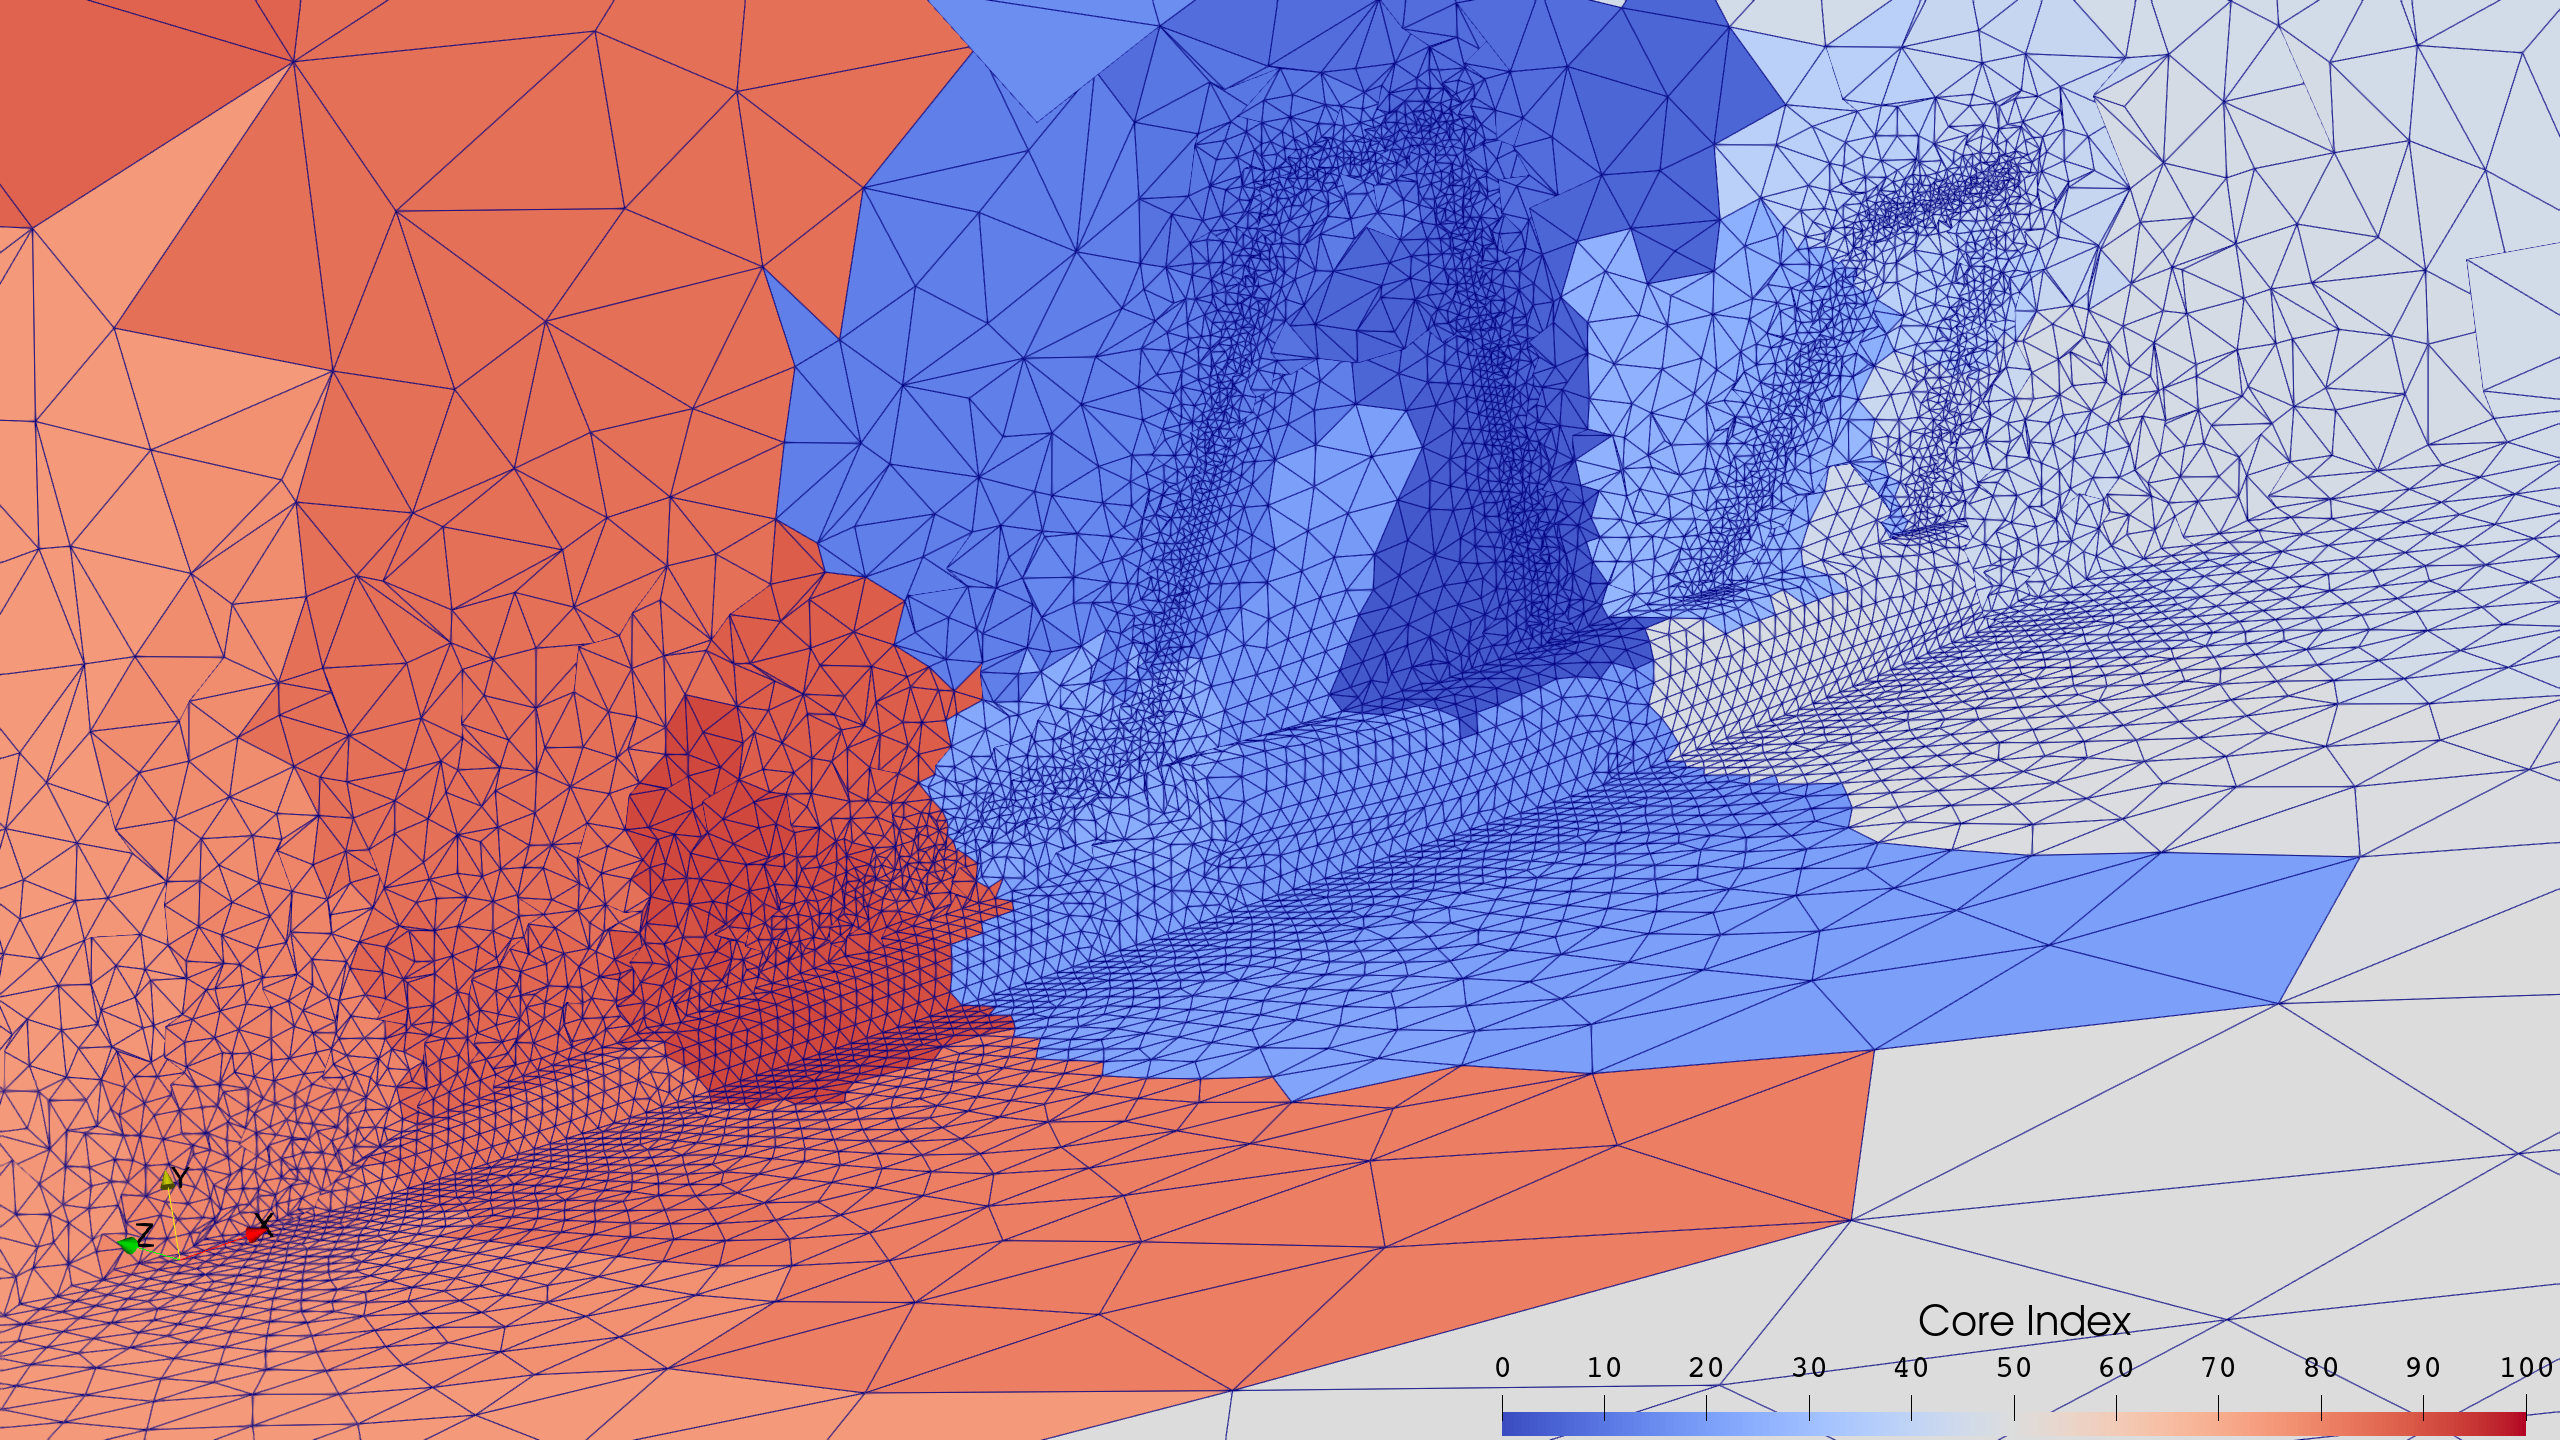
\includegraphics[width=1\textwidth]{figures/yf17/partition}

\caption{\label{fig:yf17_partition}A 100-part partitioning of the mesh used
for solving problems in Section \ref{subsec:YF-17}.}
\end{figure}

\begin{figure}
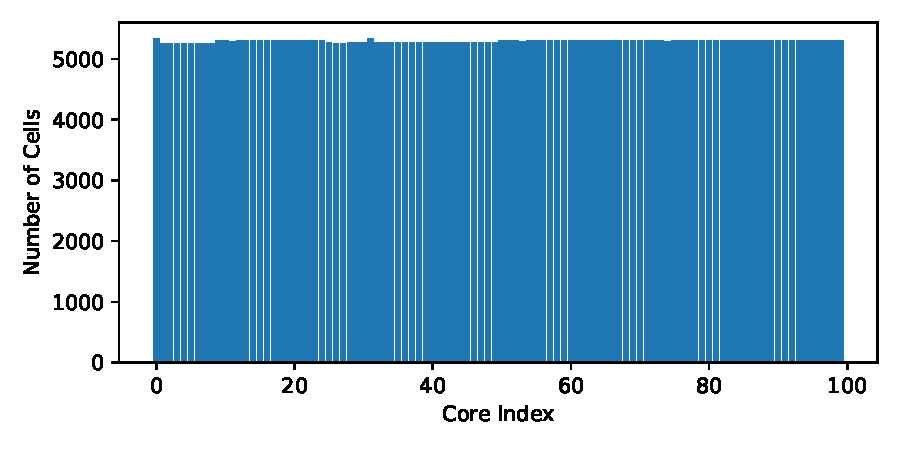
\includegraphics[width=1\textwidth]{figures/yf17/balance}

\caption{\label{fig:yf17_balance}Distribution of cells in the mesh partitioning
given in Figure \ref{fig:yf17_partition}.}
\end{figure}

Since the mesh in Figure \ref{fig:yf17_mesh} is highly unstructured
and non-uniform, simple geometric partitioning cannot achieve a relatively
balanced distribution of computational efforts. In our code, we use
the \textsc{Metis} library \citep{Karypis_1998} to partition the
dual graph of the mesh, which gives the results in Figures \ref{fig:yf17_partition}
and \ref{fig:yf17_balance}. The fluctuation of cell numbers is under
$2\%$, which is quite good since the optimal partitioning of an unstructured
mesh is an NP-hard problem. With such an approximately optimal partitioning,
the parallel efficiency, which is defined as

\[
E=\frac{T_{\text{serial}}}{PT_{\text{parallel}}}\times100\%
\]

in which $P$ is the number of processes, could surpass $99\%$ in
theory. In practice, however, the $E$ values given by our numerical
experiments are only around $80\%$ as shown in Figure \ref{fig:yf17_efficiency},
which is derived from the measured time costs given in Table \ref{tab:time_cost}.
The main reason for the gap between theory and practice is that in
the derivation of the ideal $E$ value, inter-process communications
are assumed to overlap in time with inner-cell computations, which
is an over-optimistic assumption. Nevertheless, the acceleration is
still significant, which reduces the wall clock time to an acceptable
level.

\begin{figure}
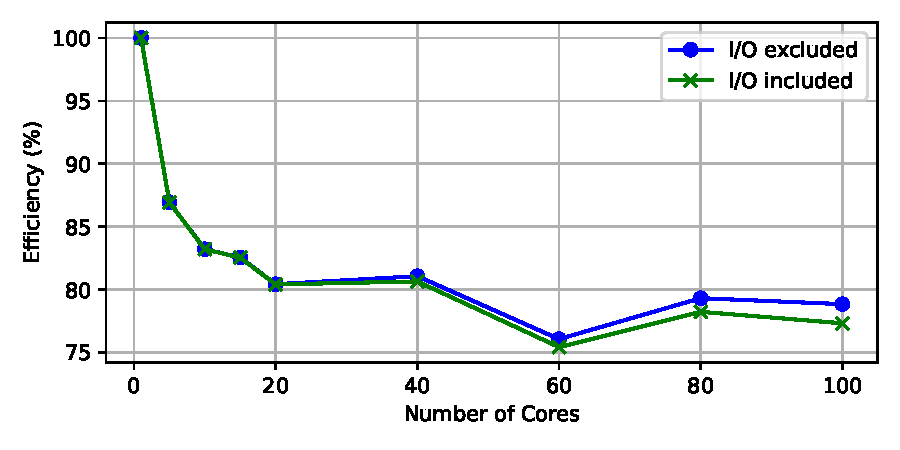
\includegraphics[width=1\textwidth]{figures/yf17/efficiency}

\caption{\label{fig:yf17_efficiency}Parallel efficiency of the third-order
solver for solving Problem \ref{prob:Supersonic-YF17}.}
\end{figure}

\begin{table}[H]
\caption{\label{tab:time_cost}Time costs of the third-order solver running
on different number of cores.}

\begin{tabular*}{1\textwidth}{@{\extracolsep{\fill}}>{\centering}p{0.1\textwidth}>{\centering}p{0.1\textwidth}>{\centering}p{0.1\textwidth}>{\centering}p{0.1\textwidth}>{\centering}p{0.1\textwidth}>{\centering}p{0.1\textwidth}}
\toprule 
\textbf{$P$} & \textbf{$T_{100}$} & \textbf{$T_{399}$} & \textbf{$T_{400}$} & $P\frac{T_{399}-T_{100}}{399-100}$ & $P\frac{T_{400}-T_{100}}{400-100}$\tabularnewline
\midrule 
1 & 10511.3 & 42466.5 & 42593.0 & 106.873 & 106.939\tabularnewline
5 & 2389.25 & 9740.13 & 9769.96 & 122.925 & 123.012\tabularnewline
10 & 1246.37 & 5086.62 & 5101.95 & 128.436 & 128.519\tabularnewline
15 & 839.554 & 3420.17 & 3430.75 & 129.462 & 129.560\tabularnewline
20 & 645.737 & 2632.32 & 2640.57 & 132.882 & 132.989\tabularnewline
40 & 325.269 & 1310.72 & 1319.73 & 131.833 & 132.595\tabularnewline
60 & 222.890 & 923.043 & 931.754 & 140.499 & 141.773\tabularnewline
80 & 168.862 & 672.439 & 681.445 & 134.736 & 136.689\tabularnewline
100 & 137.787 & 543.081 & 552.682 & 135.550 & 138.298\tabularnewline
\bottomrule
\end{tabular*}
\end{table}


\subsection{Problems with Momentum Sources\label{subsec:Problems-with-Momentum}}

In this section, we solve two problems of rotorcraft aerodynamics
using the momentum source model described in Section \ref{subsec:The-Momentum-Source}.
The problems are set to simulate wind tunnel tests of a rotor (a pair
of rotary wings), using the mesh shown in Figure \ref{fig:rotor_mesh}.
All of the boundaries of the outside box are solid walls, except he
left and right ends, which are set as inlet and outlet, respectively.
The spherical region is the circumscribed sphere of the rotor, whose
rotating axis could point to any direction. The smaller box enclosing
the sphere is used for refining the mesh in the surrounding and downstream
regions of the rotor.

\begin{figure}
\includegraphics[width=1\textwidth]{figures/rotor_in_tunnel/mesh}

\caption{\label{fig:rotor_mesh}A schematic mesh for solving problems in Section
\ref{subsec:Problems-with-Momentum}.}
\end{figure}


\subsubsection{A Climbing Rotor}
\begin{Problem}
\label{prob:rotor_upward}Solve Equation \eqref{eq:euler_system}
in the surrounding of a rotor, whose rotating axis points to the direction
of $(-1,0,0)$. The initial condition is given as a uniform flow:

\[
\begin{bmatrix}\rho & u & v & w & p\end{bmatrix}_{t=0}=\begin{bmatrix}1.29 & 1.0 & 0.0 & 0.0 & 101325.0\end{bmatrix},
\]

which is also the background state at the two ends of the wind tunnel.
\end{Problem}

\begin{figure}
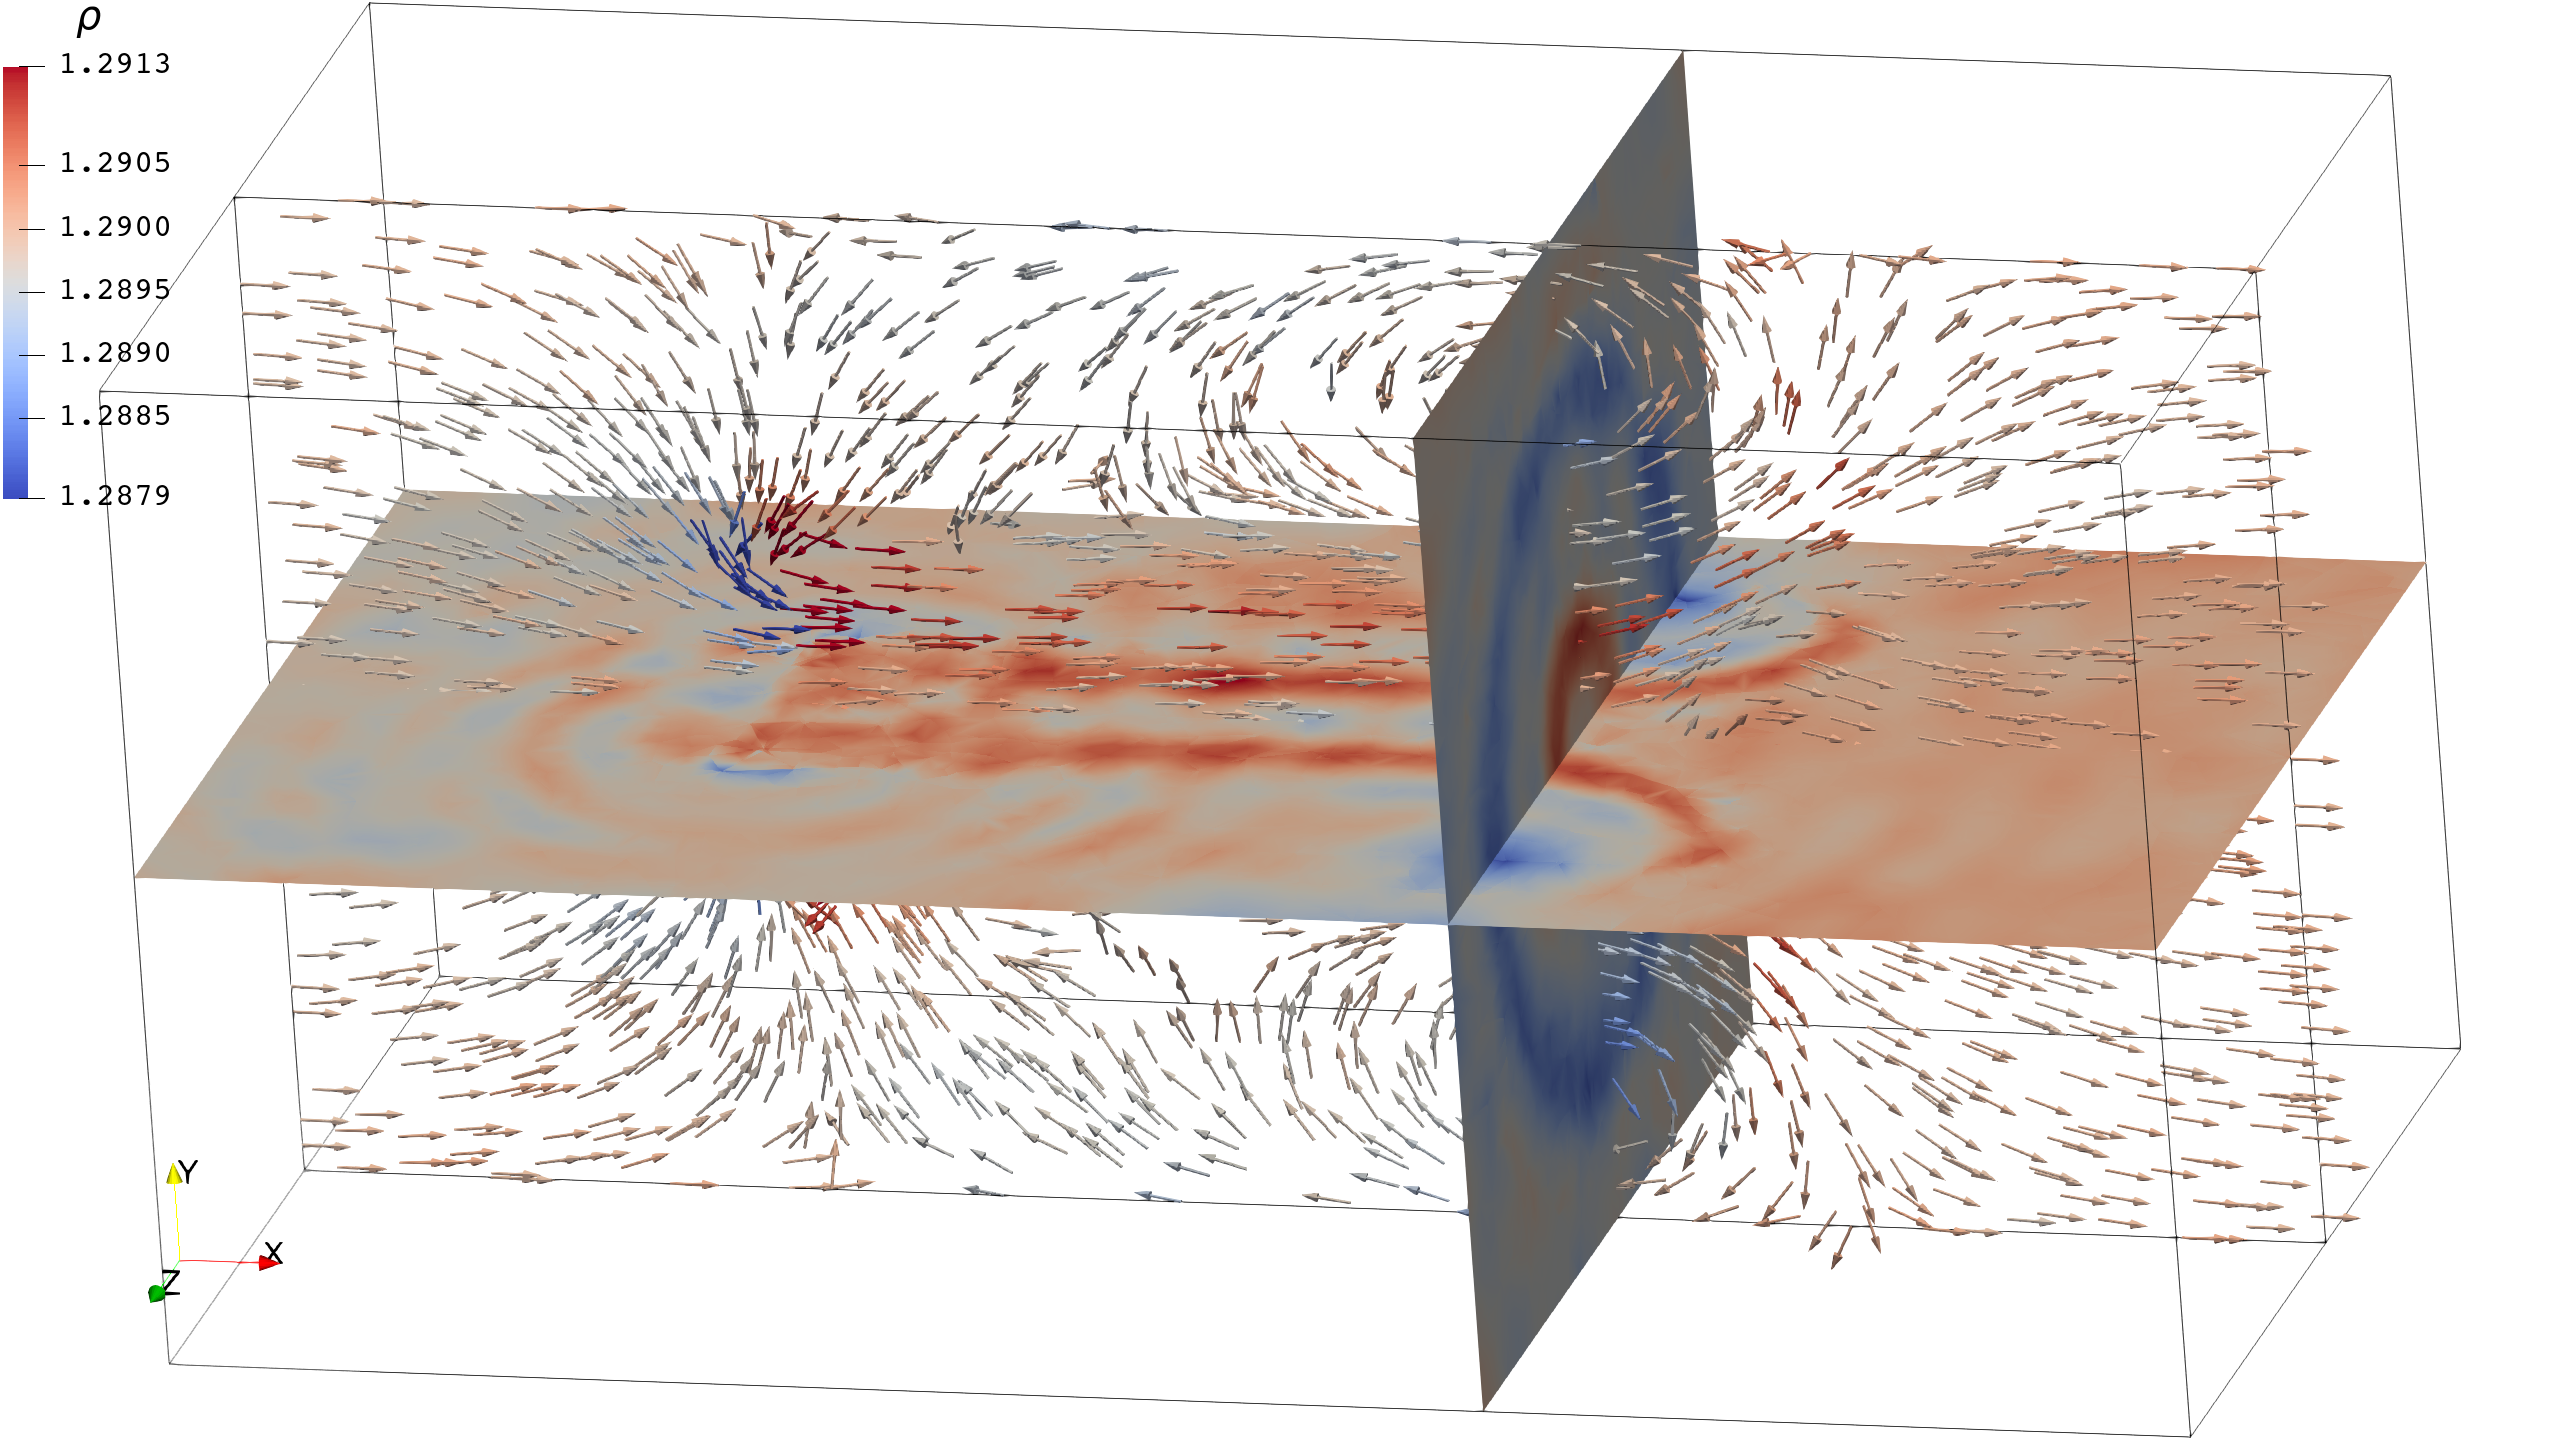
\includegraphics[width=1\textwidth]{figures/rotor_in_tunnel/upward_p=3}

\caption{\label{fig:rotor_upward_p=00003D3}Third-order solution of Problem
\ref{prob:rotor_upward} at $t=1$.}
\end{figure}

\begin{figure}
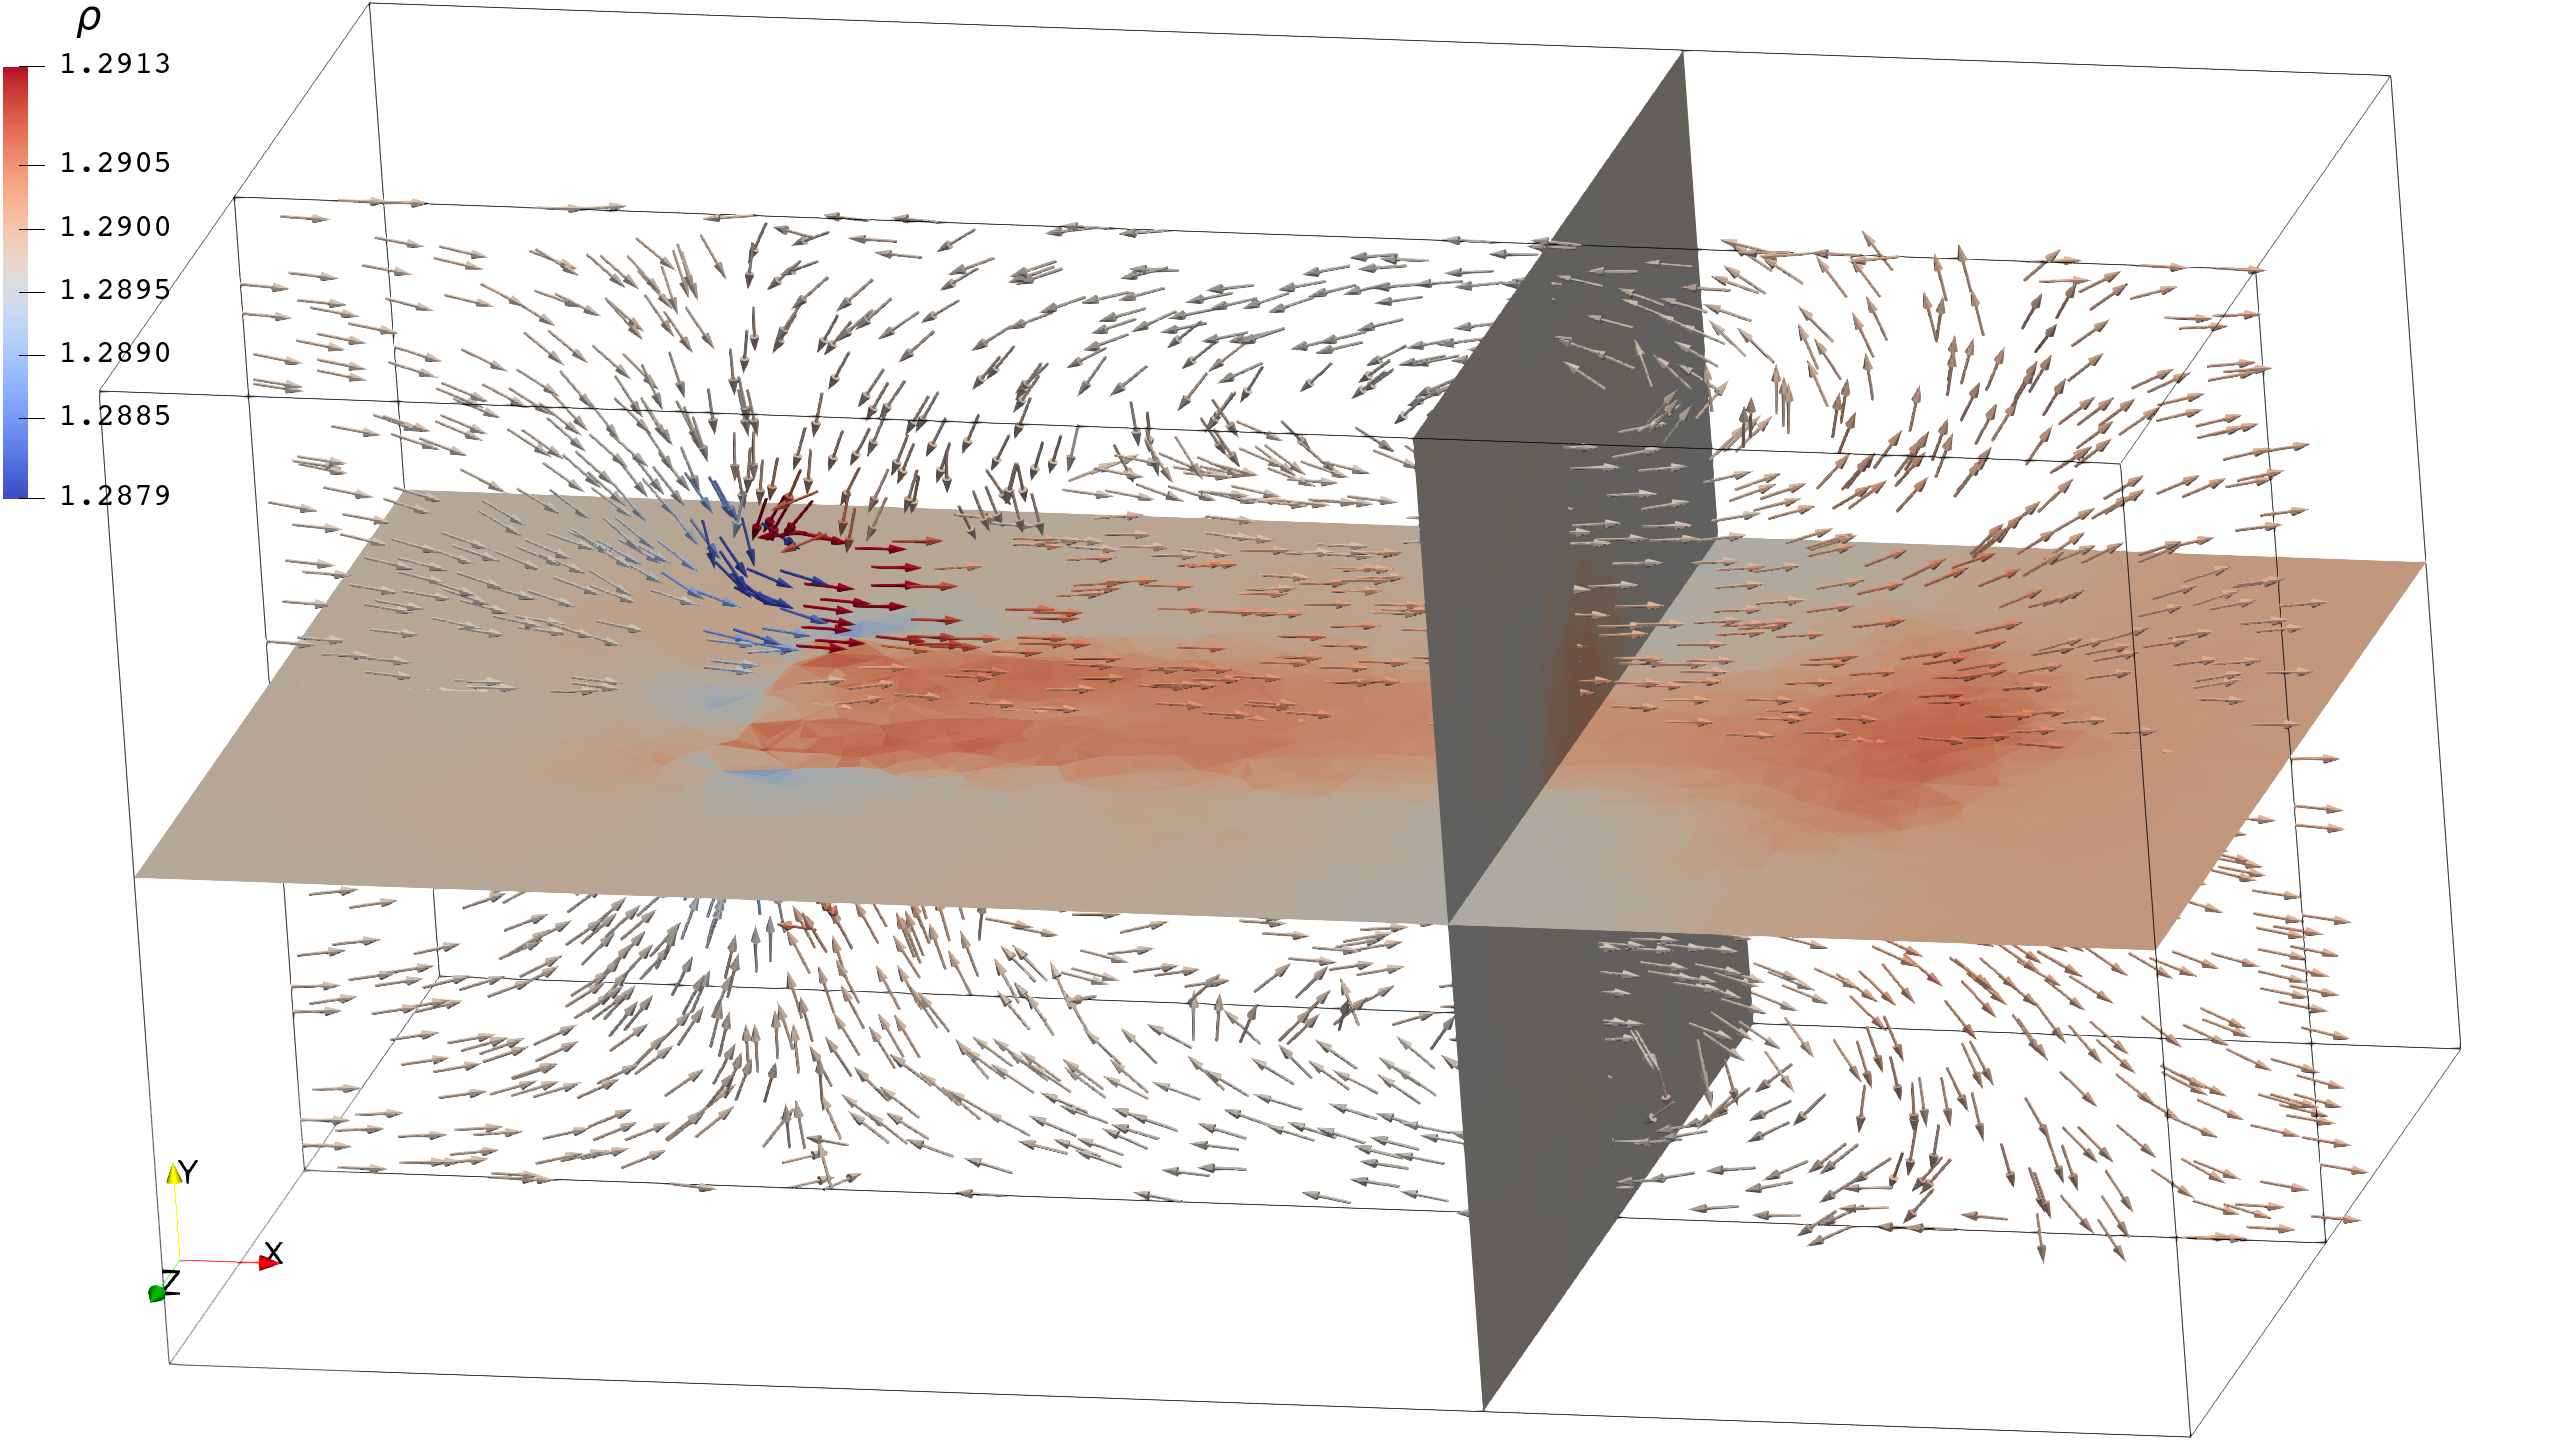
\includegraphics[width=1\textwidth]{figures/rotor_in_tunnel/upward_p=1}

\caption{\label{fig:rotor_upward_p=00003D1}First-order solution of Problem
\ref{prob:rotor_upward} at $t=1$.}
\end{figure}

Third- and first-order solutions at the same moment ($t=1$) are shown
in Figure \ref{fig:rotor_upward_p=00003D3} and Figure \ref{fig:rotor_upward_p=00003D1},
respectively, in which density contours and velocity directions are
plotted on selected slices. Large-scale flow structures, such as the
contraction of airflow near the rotor disk and the rolled-up of airwake,
are captured in both figures. However, finer details, such as the
ripples generated from the rotor disk and the strong vortex ring in
the downstream, are only visible in the third-order solution. The
nearly axisymmetric flow structure is caused by the periodic movement
of the rotary wings. The density of air just below the rotor (red)
is greater than that above the rotor (blue), which means the rotor
is compressing the air flowing across it. According to Newton's third
law, the rotor must be experiencing a force in the opposite direction
exerted by the air. This is where the rotor thrust comes from.

\subsubsection{A Rotor in Forward Flight}
\begin{Problem}
\label{prob:rotor_forward}Solve Equation \eqref{eq:euler_system}
in the surrounding of a rotor, whose rotating axis points to the direction
of $(0,0,1)$. The initial condition is given as a uniform flow:

\[
\begin{bmatrix}\rho & u & v & w & p\end{bmatrix}_{t=0}=\begin{bmatrix}1.29 & 10.0 & 0.0 & 0.0 & 101325.0\end{bmatrix},
\]

which is also the background state at the two ends of the wind tunnel.
\end{Problem}

\begin{figure}
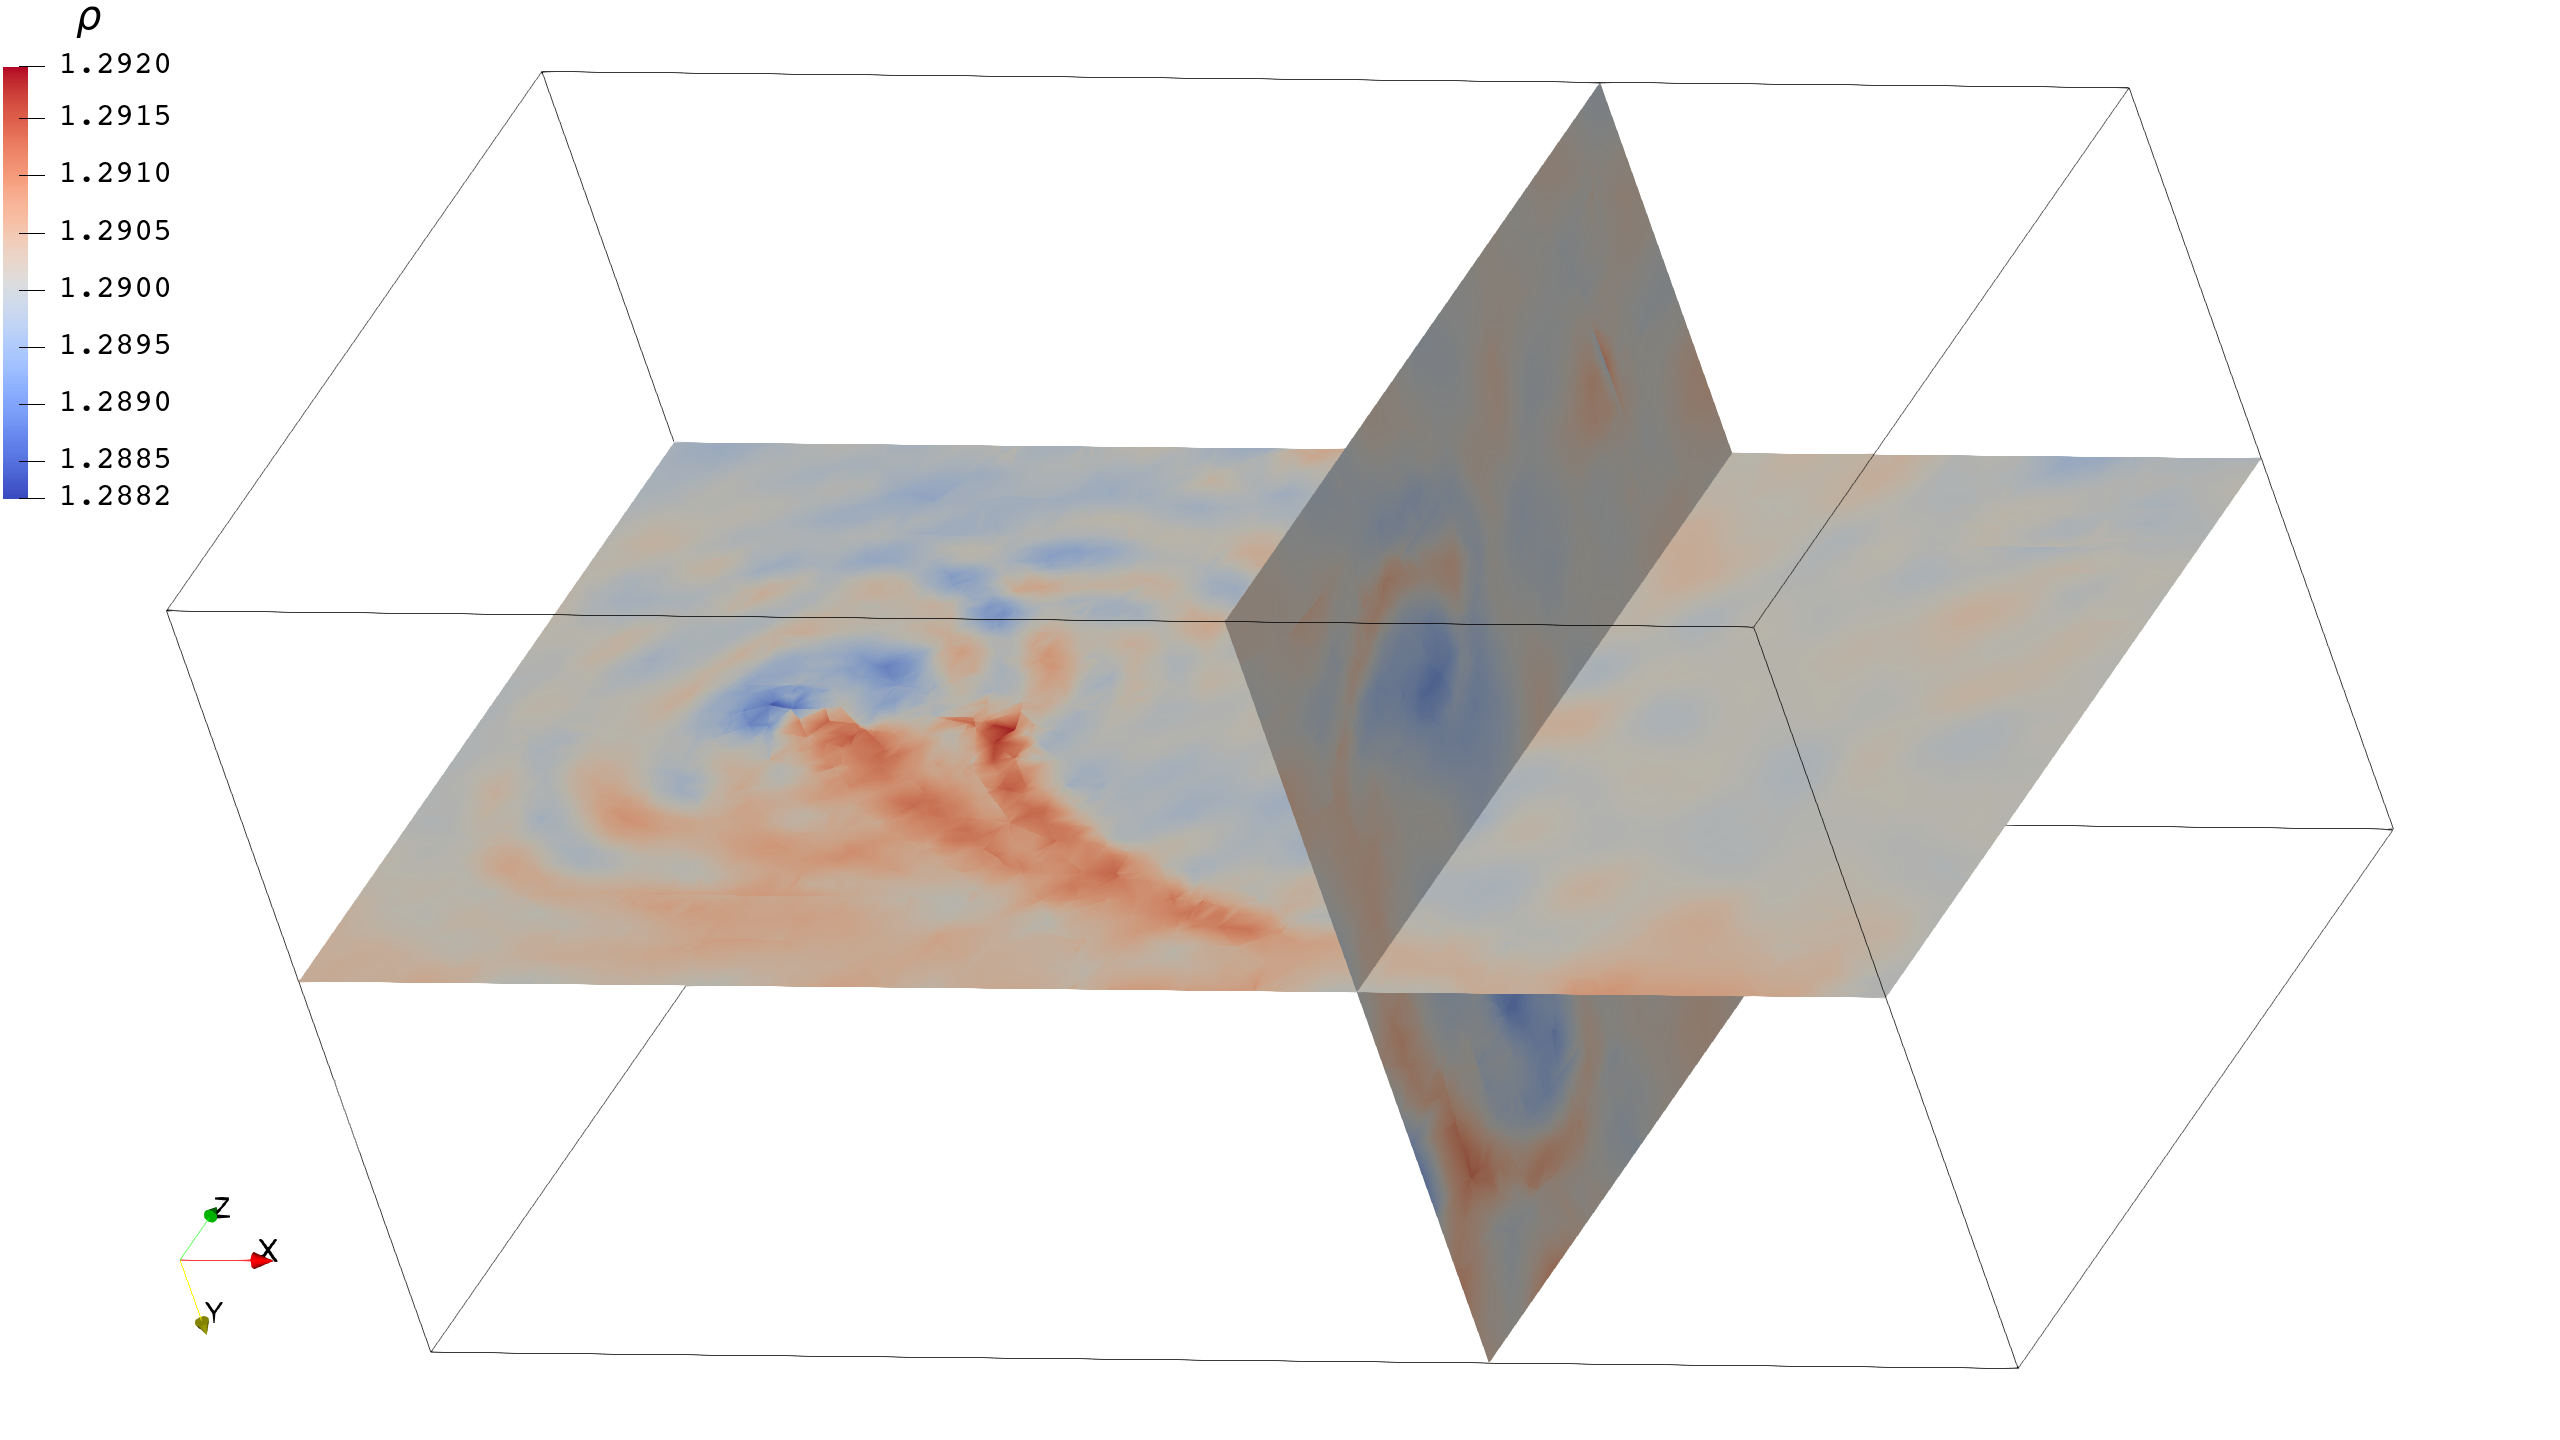
\includegraphics[width=1\textwidth]{figures/rotor_in_tunnel/forward_p=3}

\caption{\label{fig:rotor_forward_p=00003D3}Third-order solution of Problem
\ref{prob:rotor_forward} at $t=1$.}
\end{figure}

\begin{figure}
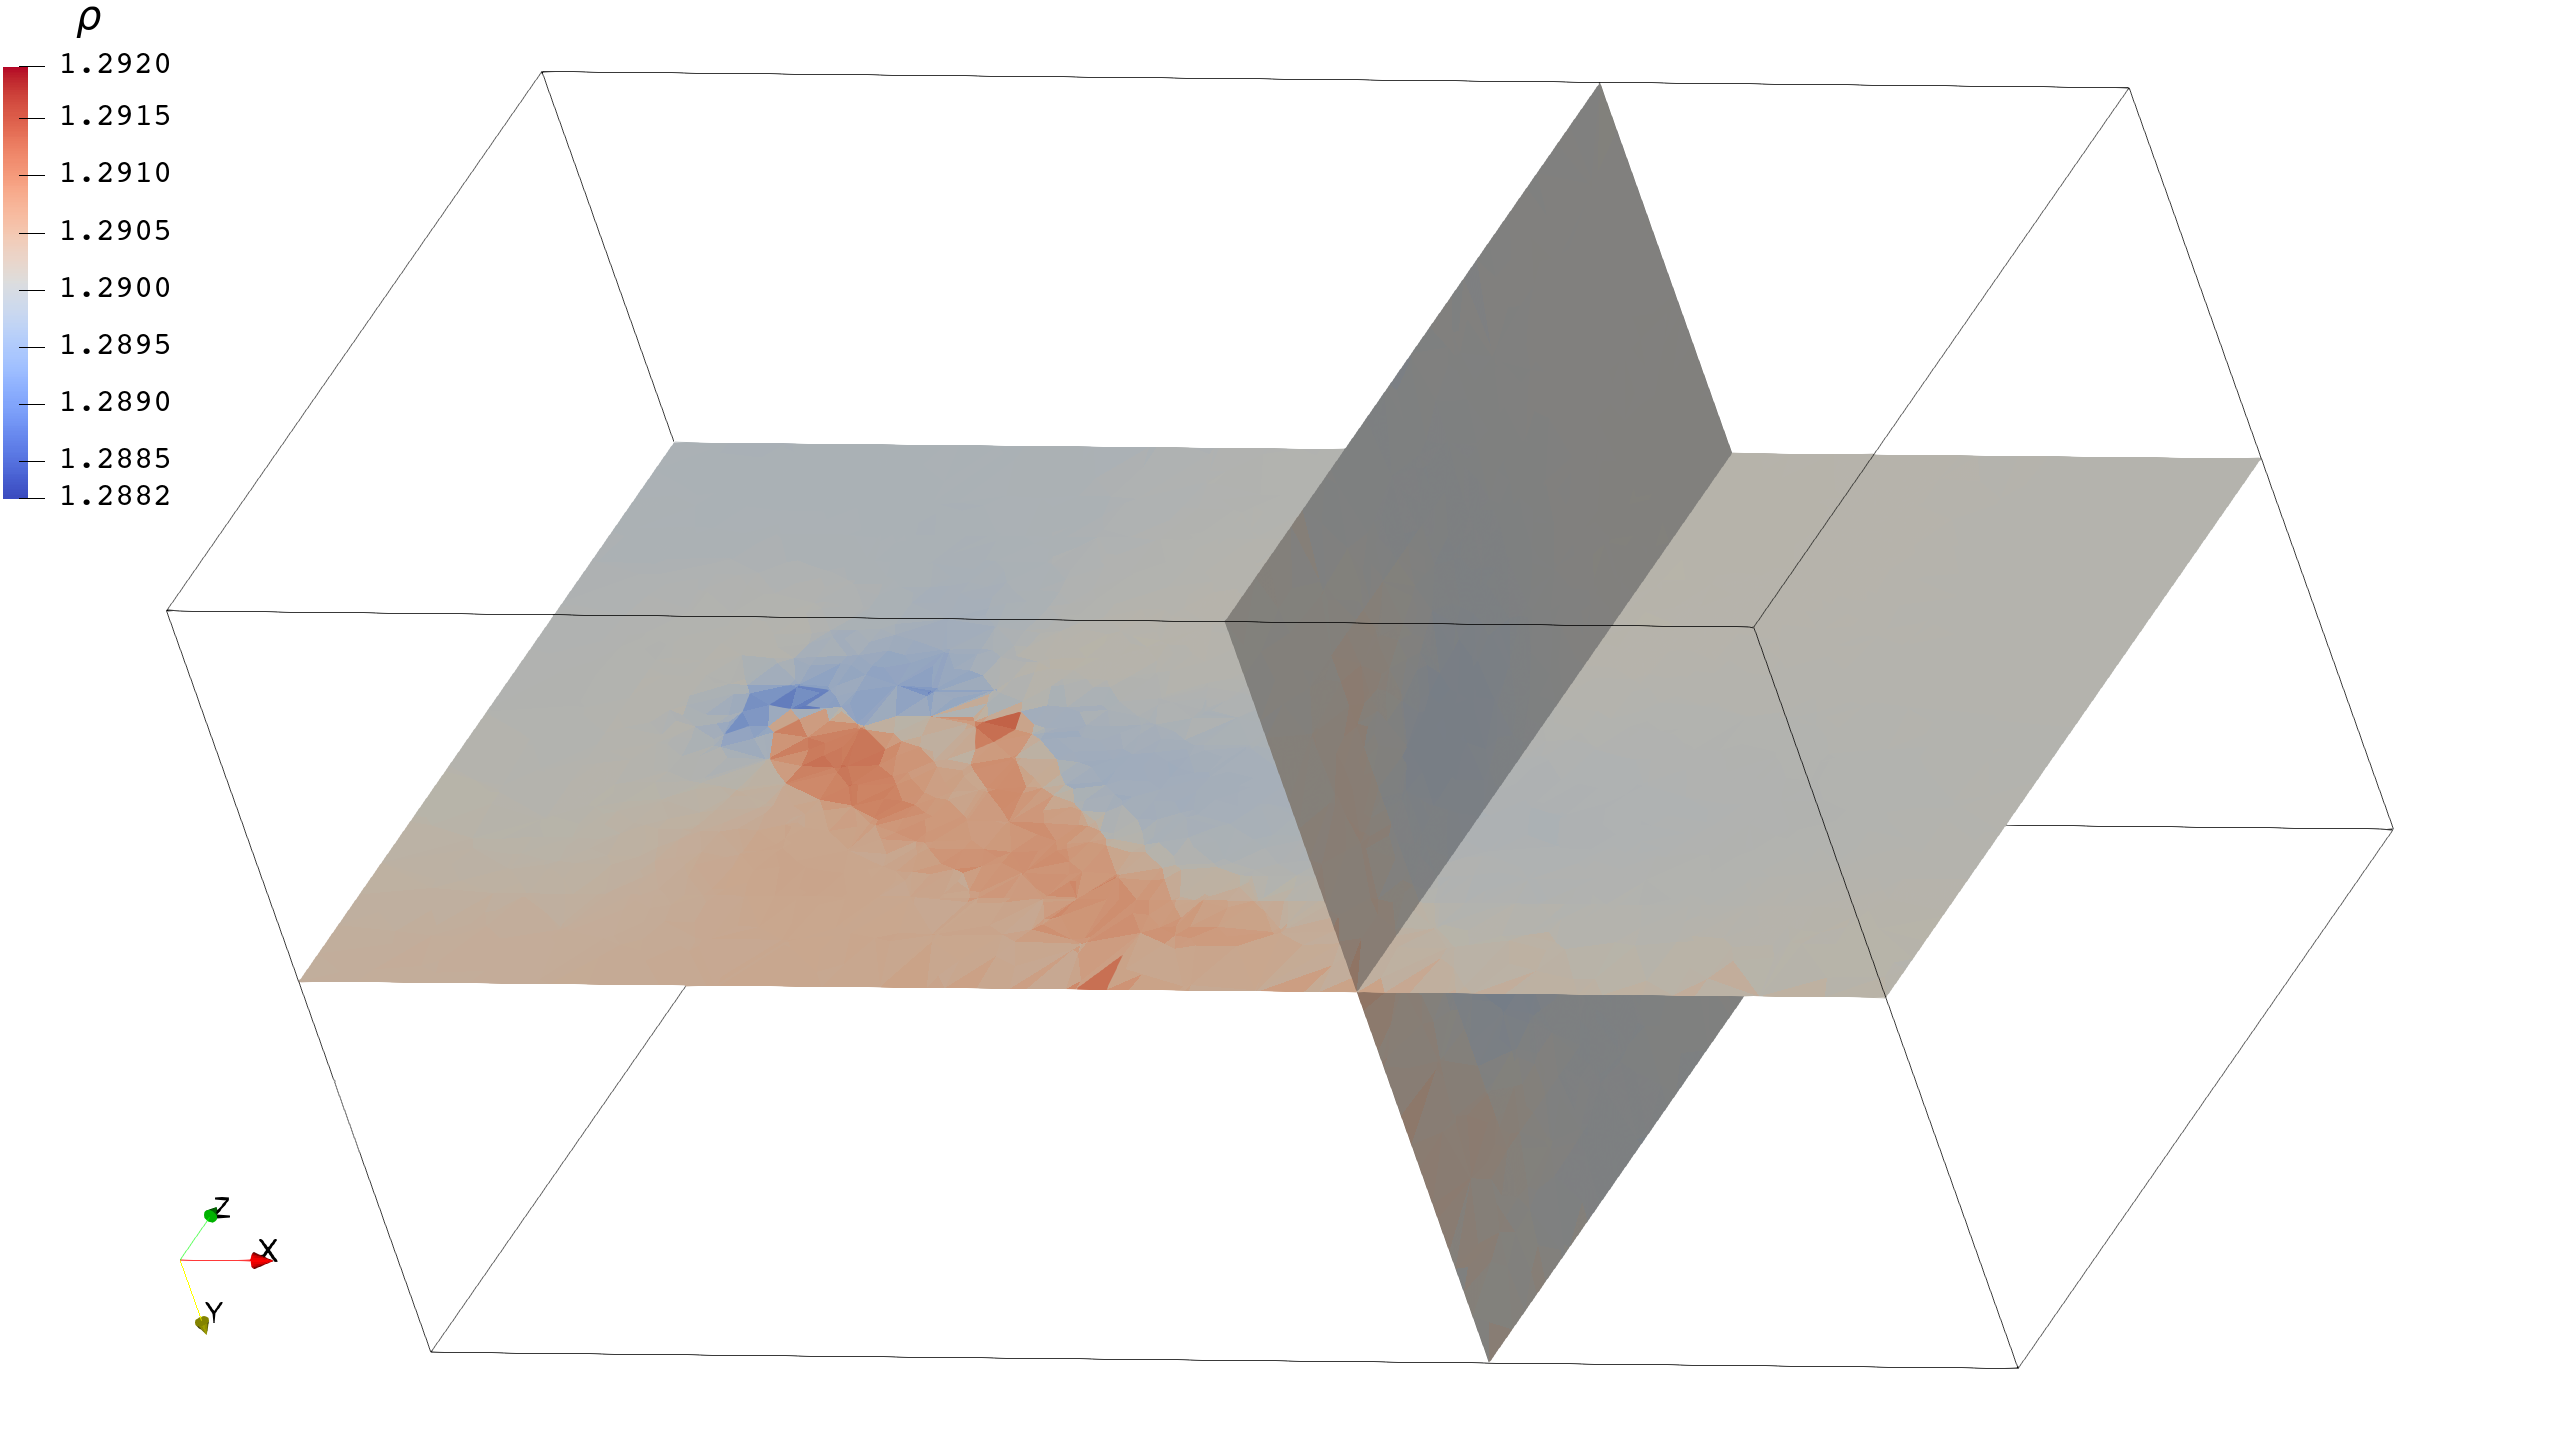
\includegraphics[width=1\textwidth]{figures/rotor_in_tunnel/forward_p=1}

\caption{\label{fig:rotor_forward_p=00003D1}First-order solution of Problem
\ref{prob:rotor_forward} at $t=1$.}
\end{figure}

\begin{figure}
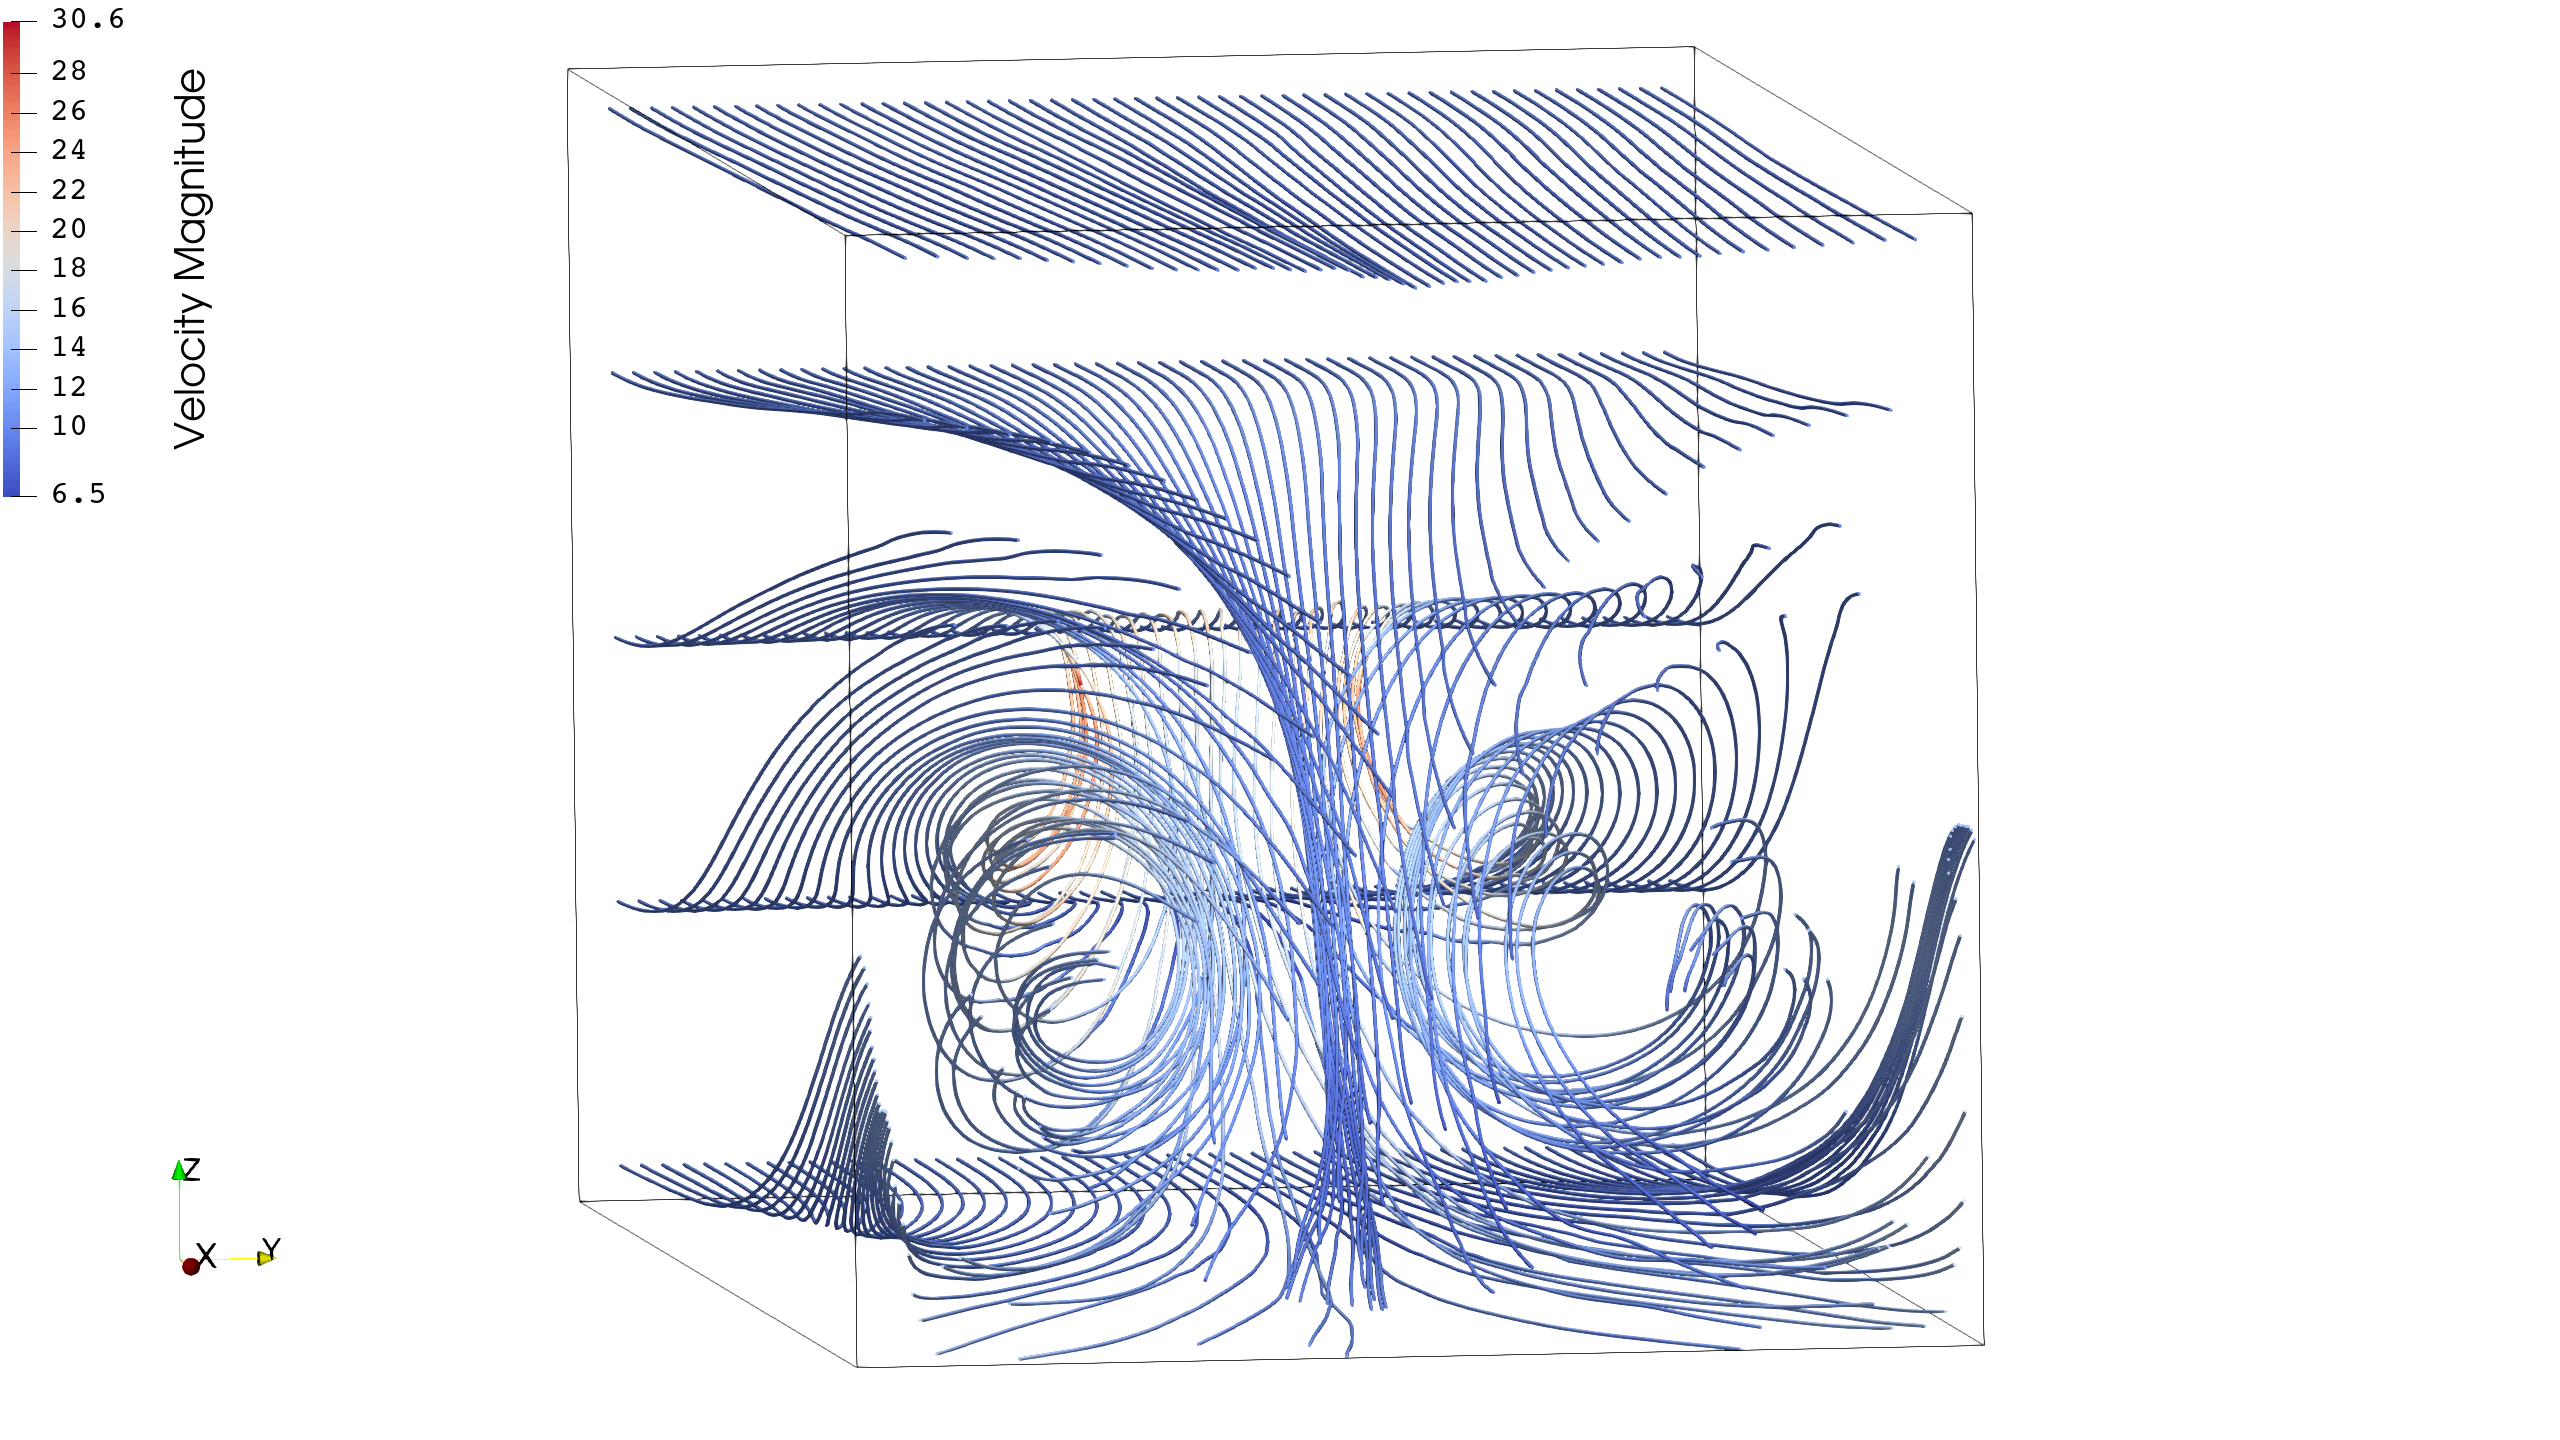
\includegraphics[width=1\textwidth]{figures/rotor_in_tunnel/forward_wake_p=3}

\caption{\label{fig:rotor_forward_wake}Streamlines of the solution in Figure
\ref{fig:rotor_forward_p=00003D3}.}
\end{figure}

Just like the climbing problem, we plot the third- and first-order
solution at the same moment ($t=1$) in Figure \ref{fig:rotor_forward_p=00003D3}
and Figure \ref{fig:rotor_forward_p=00003D1}, respectively. As before,
both of them can capture large-scaled structures, such as the skewed
and rolled-up airwakes. The rolled-up structure is more clear in Figure
\ref{fig:rotor_forward_wake}, in which streamlines of are ploted
and colorred by the magnitude of velocity. The piecewise constant
first-order solution is much vaguer and losts many details, which
shows again the value of developing high-order solvers.

\section{Discussion}

In this article, we give a concise but complete formulation of an
RKDG scheme with a compact WENO limiter for solving inviscid compressible
flows, possibly with momentum sources, on three-dimensional unstructured
meshes. The algorithms are implemented on top of public available
libraries, which support unstructured mesh partitioning, inter-process
communication and distributed memory parallelization. The correctness
and accuracy of the solvers are validated by lower-dimensional reference
problems. Results of real three-dimensional applications are also
presented, in which complex flow structures are captured by the third-order
solver even on very coarse unstructured meshes. Future works may include
implementing higher-order solvers under the this framework and testing
them on larger meshes and on larger high-performance computing platforms.

\vspace{6pt}


\authorcontributions{Conceptualization, W.P. and S.L.; methodology, W.P.; software, W.P.
and Y.J.; validation, W.P. and Y.J.; formal analysis, W.P. and Y.J.;
investigation, W.P.; resources, W.P.; data curation, W.P.; writing-{}-{}-original
draft preparation, W.P.; writing-{}-{}-review and editing, W.P., Y.J.
and S.L.; visualization, W.P.; supervision, S.L.; project administration,
S.L.; funding acquisition, S.L. All authors have read and agreed to
the published version of the manuscript.}

\funding{This research was funded by the National High-tech R\&D Program of
China (863 Program) grant number 2012AA112201.}

\institutionalreview{Not applicable.}

\informedconsent{Not applicable.}

\dataavailability{The data presented in this article are all generated from the source
code publicly available in our Git repository \url{https://github.com/pvc1989/miniCFD}
(or the mirror site \url{https://gitee.com/pvc1989/miniCFD}), except
the mesh used in Section \ref{subsec:YF-17} which is downloaded from
\url{https://cgns.github.io/CGNSFiles.html}.}

\acknowledgments{The authors would like to express the deepest appreciation to Shen
Xin for his professional guidance on computer science, and to Zhou
Yukai for his patient assistance on mathtyping.}

\conflictsofinterest{The authors declare no conflict of interest. The funders had no role
in the design of the study; in the collection, analyses, or interpretation
of data; in the writing of the manuscript, or in the decision to publish
the~results.}

\abbreviations{Abbreviations}{The following abbreviations are used in this manuscript:\\

\noindent%
\begin{tabular}{@{}ll}
CFD & Computational Fluid Dynamics\tabularnewline
FD & Finite Difference\tabularnewline
FV & Finite Volume\tabularnewline
FE & Finite Element\tabularnewline
DG & Discontinuous Galerkin\tabularnewline
RK & Runge--Kutta\tabularnewline
TVD & total variation diminishing\tabularnewline
SSP & strong stability-preserving\tabularnewline
ENO & Essentially Non-Oscillatory\tabularnewline
WENO & Weighted ENO\tabularnewline
\end{tabular}}

\abbreviations{Nomenclature}{The following symbols are used in this manuscript:\\

\noindent%
\begin{tabular}{@{}ll}
$\partial_{t},\partial_{x},\partial_{y},\partial_{z}$ & partial derivative with respect to $t,x,y,z$\tabularnewline
$\alpha$ & angle of attack\tabularnewline
$\gamma$ & heat capacity ratio of the gas\tabularnewline
$\vec{\nu}$ & outer normal vector at some point on $\partial E_{i}$\tabularnewline
$\vec{\pi},\vec{\sigma}$ & tangential vectors at some point on $\partial E_{i}$\tabularnewline
$\rho$ & density of the gas\tabularnewline
$\phi_{k}$ & $k$-th function in an orthonormal basis\tabularnewline
$\psi$ & an arbitrary test function\tabularnewline
$\psi^{h}$ & approximation of $\psi$\tabularnewline
$\hat{\psi}_{k}$ & projection of $\psi$ on $\phi_{k}$\tabularnewline
$\underline{A^{\nu}}$ & Jacobian of $\underline{F^{\nu}}$ with respect to $\underline{U}$\tabularnewline
$\vec{b}_{L}$  & body force per unit length\tabularnewline
$\vec{b}_{V}$ & body force per unit volume\tabularnewline
$b_{x},b_{y},b_{z}$ & $x,y,z$-component of body force per unit volume\tabularnewline
$c$ & chord length of a blade\tabularnewline
$E_{i}$ and $\partial E_{i}$ & $i$-th element (cell) and its boundary\tabularnewline
$e_{0}$ & specific total energy of the gas\tabularnewline
$\underline{\vec{F}}$ & flux tensor\tabularnewline
$\underline{F^{\nu}}$ & projection of $\underline{\vec{F}}$ on $\vec{\nu}$\tabularnewline
$\underline{F^{x}},\underline{F^{y}},\underline{F^{z}}$ & $x,y,z$-component of $\underline{\vec{F}}$\tabularnewline
$h_{0}$ & specific total enthalpy of the gas\tabularnewline
$p$ & pressure of the gas\tabularnewline
$\underline{Q}$ & column matrix of source terms\tabularnewline
$\underline{R}$ & changing rate of $\underline{\hat{U}}$\tabularnewline
$\underline{R^{\nu}}$ & matrix whose $j$-th column is the $j$-th eigenvector of $\underline{A^{\nu}}$\tabularnewline
$\underline{U}$ & column matrix of conservative variables\tabularnewline
$\underline{U}^{h}$ and $\underline{U}^{\text{new}}$ & approximation of $\underline{U}$ and its WENO reconstruction\tabularnewline
$\underline{U}_{i|k}^{\text{new}}$ & WENO reconstruction of $\underline{U}^{h}$ on $E_{i}$ with the help
of $E_{k}$\tabularnewline
$\underline{\hat{U}}$ & coefficient matrix whose $k$-th column is $\underline{\hat{U}}_{k}$\tabularnewline
$\underline{\hat{U}}_{k}$ & projection of $\underline{U}$ on $\phi_{k}$\tabularnewline
$\underline{\hat{U}}^{n}$ & $\underline{\hat{U}}$ and at the $n$-th time step\tabularnewline
$u_{x},u_{y},u_{z}$ & $x,y,z$-component of velocity\tabularnewline
$\underline{V}$ & column matrix of characteristic variables\tabularnewline
$\underline{V}^{h}$ and $\underline{V}^{\text{new}}$ & approximation of $\underline{V}$ and its WENO reconstruction\tabularnewline
\end{tabular}}

\appendixtitles{no}

\appendixstart{}

\appendix

\begin{adjustwidth}{-\extralength}{0cm}{}


\reftitle{References}


\externalbibliography{yes}

\bibliography{reference}

%%%%%%%%%%%%%%%%%%%%%%%%%%%%%%%%%%%%%%%%%%
%% for journal Sci
%\reviewreports{\\
%Reviewer 1 comments and authors' response\\
%Reviewer 2 comments and authors' response\\
%Reviewer 3 comments and authors' response
%}
%%%%%%%%%%%%%%%%%%%%%%%%%%%%%%%%%%%%%%%%%%

\end{adjustwidth}{}


\end{document}
